\documentclass[final]{uclthesis} %final draft web
\RequirePackage{uclthesis}

% PDF metadata
\makeatletter
\@ifpackageloaded{hyperref}{%
  \hypersetup{%
    pdftitle = {Jet physics with the \ATLAS experiment at the \LHC},
    pdfsubject = {James Robinson's PhD thesis},
    pdfkeywords = {ATLAS, forward, jet, physics, LHC},
    pdfauthor = {\textcopyright\ James Robinson}
  }
}{}
\makeatother

%% Define the thesis title and author
\title{Jet physics with the \ATLAS experiment at the \LHC}
\author{James Edward Martyn Robinson\xspace}
\date{March 28th, 2012}

%% Start the document
\begin{document}

%% Define the un-numbered front matter (cover pages, rubric and table of contents)
\begin{frontmatter}
  \input{structure/frontmatter}
\end{frontmatter}

%% Start the content body of the thesis
\begin{mainmatter}
  % To build feynmf files, run 'make' once then do: mf '\mode=localfont; input $name'
\chapter{Theoretical Framework}
\label{chap:bg-theory}

\chapterquote{I am now convinced that theoretical physics is actually philosophy.}
{Max Born}

\section{Quantum Chromodynamics}
Quantum chromodynamics (\QCD) is the non-Abelian \SUgroup{3} gauge theory of the strong interaction.
Initially, it appears similar to \QED, with the single electric charge replaced by three conserved ``colour'' charges; there are, however, important differences between the two.

In the \QED Lagrangian, \EquationRef{eq:bg-theory:qed}, the electron carries one unit of charge, $-e$, the positron carries one unit of anti-charge $+e$ and the force is mediated by a massless photon.

\begin{gather}
  \label{eq:bg-theory:qed}
  \Lagrangian_{\QED} = \bar{\psi} \left(i \gamma^{\mu}  \partial_{\mu} -m \right) \psi - e \bar{\psi} \gamma^{\mu} A_{ \mu} \psi - \frac{1}{4}F_{\mu\nu}F^{\mu\nu}
  \intertext{where for a photon field $A_{\mu}$,}
  F_{\mu\nu} = \partial_{\mu} A_{\nu} - \partial_{\nu} A_{\mu} \nonumber
\end{gather}

Similarly, in the \QCD Lagrangian, \EquationRef{eq:bg-theory:qcd}, the quarks carry colour charge, $r, g, b$, anti-quarks carry anti-charge, $\bar{r}, \bar{g}, \bar{b}$ and the force is mediated by massless gluons.
As this is an exact \SUgroup{3} symmetry, the strong interaction is invariant under rotations in
colour space.

\begin{gather}
  \label{eq:bg-theory:qcd}
  \Lagrangian_{\QCD} = \bar{\psi}_{q,a} \left(i \gamma^{\mu}  \partial_{\mu} \delta_{ab} - m \delta_{ab} \right) \psi_{q,b} - \gQCD G^A_{\mu} \left( \bar{\psi}_{q,a} \gamma^{\mu} T^{ab}_A \psi_{q,b} \right) - \frac{1}{4}F^A_{\mu\nu}F_A^{\mu\nu}
  \intertext{where for a gluon field $G^A_{\mu}$,}
  F^A_{\mu\nu} = \partial_{\mu} G^A_{\nu} - \partial_{\nu} G^A_{\mu} - \gQCD f_{ABC} G^B_{\mu} G^C_{\nu} \nonumber
\end{gather}

In \EquationRef{eq:bg-theory:qcd}, the $\gamma^{\mu}$ are the Dirac $\gamma$-matrices and repeated indices are summed over, following the Einstein summation convention.
The $\psi$ are quark-field spinors for a quark of flavour $q$ and mass $m_q$, with a colour-index $a$ that runs from $a = 1$ to $N_c = 3$; quarks form the
fundamental representation of the \SUgroup{3} colour group.
The $G^A$ correspond to the gluon fields, with $A$ running from $1$ to $N_c^2-1 = 8$; there are eight types of gluon, forming the adjoint representation of the \SUgroup{3} colour group.
The $T^{ab}_A$ are eight $3 \times 3$ matrices, which form the generators of the \SUgroup{3} group, corresponding to the fact that the interaction between
a gluon and a quark rotates the quark in colour space.
Finally, \gQCD is the \QCD coupling constant and $F^A_{\mu\nu}$ the field tensor, where $f_{ABC}$ are the structure functions of the \SUgroup{3}.

In \QED, photons are electrically neutral and hence do not carry the charge of the EM interaction.
In contrast, gluons do carry colour charge, one unit of colour and one of anti-colour, so gluon self-interactions are to be expected.
Considering only the quark and gluon interaction terms the following simplified model of the \QCD Lagrangian can be obtained:

\begin{equation}
  \label{eq:bg-theory:qcd_simplified}
  \Lagrangian_{\QCD} = ``\qqbar" + ``G^{2}" + \gQCD``\qqbar G" + \gQCD``G^{3}" + \gQCD^{2}``G^{4}"
\end{equation}

Here, the $q$ correspond to quarks and the $G$ to gluons, with each term representing an allowed interaction or propagator within \QCD; the $G^3$ and $G^4$ terms represent triple and quartic gluon vertices.
The non-abelian $G^A_{\mu\nu}$ term in the Lagrangian, which gives rise to these terms, is thus the major reason for the greater complexity of \QCD in comparison to \QED.
As a result of gluon self-interactions, a \QCD process contains more diagrams at a given order than would be true for \QED.

\section{Asymptotic Freedom}
The interactions permitted by the \QCD Lagrangian mean that a quark or a gluon can emit a gluon, while gluons can make quark or gluon loops.
Analogously to \QED, these interactions are governed by a coupling constant, with $\alphaS = \frac{\gQCD^2}{4\pi}$.

Just as is the case with electric charge screening in \QED, the sum of the infinite series of higher order diagrams is equivalent to a single diagram with a ``running'' coupling constant.
However, in contrast to \QED, \alphaS \emph{decreases} with increasing \Qsquared, as can be seen in \EquationRef{eq:bg-theory:running_alpha_S}, resulting in ``anti-screening'' of colour charge.

\begin{gather}
  \label{eq:bg-theory:running_alpha_S}
  \alphaS\left(\Qsquared\right) \simeq \frac{\alphaS\left(Q_0^2\right)}{1 + B \alphaS\left(Q_0^2\right) \ln\left({\frac{\Qsquared}{Q_0^2}}\right)}
  \intertext{where for $N_c$ colours and $N_f$ quark flavours, the constant, $B$, is given by}
  B = \frac{11N_c - 2N_f}{12\pi} \nonumber
\end{gather}

At high \Qsquared, or equivalently at small distances, the effect of these higher order interactions can be conceptualised as spreading out the colour charge of an object into a ``colour cloud''.
A test charge inside the colour cloud will experience a smaller force than if it were a large distance away.
At small distances, therefore, quarks interact through colour fields of reduced strength and asymptotically behave like free particles. This phenomenon is known as asymptotic freedom and allows perturbation theory to be used in this region, permitting high precision tests, similar to those possible in \QED~\cite{Martin:2009:Nuclear}.

\section{Colour Confinement}
It is believed, although not yet proven, that all observable free particles must be colourless.
This is known as the colour confinement hypothesis: only colour singlet states can exist as free particles.
Consequently quarks are never observed in isolation but only in bound states as colourless hadrons.
Any energy injected into a hadron does not separate the quarks, but goes into creating \qqbar pairs and hence further hadrons.

\begin{figure}[htpb]
  \subfloat[Field lines arising from a \QED dipole]{
    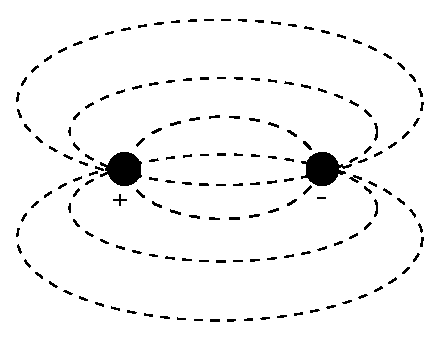
\includegraphics[width=\tinyfigwidth]{chapters/bg-theory/QEDDipoles.eps}
    \label{fig:bg-theory:qeddipole}}
  \qquad
  \subfloat[Field lines arising from a \QCD dipole]{
    \includegraphics[width=\tinyfigwidth]{chapters/bg-theory/QCDTube.eps}
    \label{fig:bg-theory:qcddipole}}
  \caption{A comparison of the fields between \QED (electric) and \QCD (colour) dipoles: \protect\subref{fig:bg-theory:qeddipole} the electric field surrounding two opposite electric charges and \protect\subref{fig:bg-theory:qcddipole} the colour field surrounding a \qqbar pair  are shown. In comparison to the \QED case, the lines of force in \QCD are compressed. As the \qqbar separation, $r$, is increased, the \xs{al} area of the \QCD ``flux tube'' remains constant.}
  \label{fig:bg-theory:qedqcddipoles}
\end{figure}

Gluon self-interactions provide a plausible means by which colour confinement could arise.
When two coloured objects separate, the exchange of virtual gluons ``squeezes'' the lines of force between them so that they are closer together than in the \QED case and a ``flux tube'' of interacting gluons is formed (see \FigureRef{fig:bg-theory:qedqcddipoles}).
As the distance, $r$, between them increases, the \xs area of this tube remains approximately constant.
Since the number of field lines depends only on the colour of the sources, the field strength in the tube must also remain constant, while the field energy grows in proportion to the volume of the tube.
This means that the energy of the \qqbar system increases linearly with separation and hence that it would require an infinite amount of energy to fully separate two coloured objects~\cite{Gottfried:1986:concepts}.

\section{Evolution Equations}
\subsection{Deep Inelastic Scattering and the Quark-Parton Model}
The process in which the lepton from an \ep collision interacts with a quark from the proton is known as deep inelastic scattering (DIS).
If the interacting quark carries a fraction, $x$ of the proton's 4-momentum, $p$, then the \xs for this process is given by
%%The process in which the lepton from an \ep collision interacts with
%%a quark from the proton is known as deep inelastic scattering (DIS).

%%\begin{figure}[htpb]
%%  \parbox{100mm}{
%%    \vspace*{5mm}
%%    \unitlength=1mm
%%    \begin{fmffile}{dis}
%%      \begin{fmfgraph*}(100,50)
%%        \fmfleft{ip,il}
%%        \fmfright{oq1,oq2,d1,oq3,d2,d3,ol}
%%        \fmf{fermion}{ip,vp}
%%        \fmf{fermion,label=q $(xp)$}{vp,vq}
%%        \fmf{fermion,label=q $(p')$}{vq,oq3}
%%        \fmf{phantom}{ip,vp}
%%        \fmf{fermion}{vp,oq1}
%%        \fmf{fermion}{vp,oq2}
%%        \fmf{photon,tension=0.9,label=$\gamma / Z^{0} / W^{\pm} (q)$}{vl,vq}
%%        \fmf{fermion}{il,vl,ol}
%%        \fmf{phantom}{il,vl}
%%        \fmfblob{.15w}{vp}
%%        \fmfdot{vq,vl}
%%        \fmffreeze
%%        \fmfi{plain}{vpath (__ip,__vp) shifted (thick*(0,2))}
%%        \fmfi{plain}{vpath (__ip,__vp) shifted (thick*(1,-2))}
%%        \fmflabel{P ($p$)}{ip}
%%        \fmflabel{$e^{\pm}$ ($k$)}{il}
%%        \fmflabel{lepton}{ol}
%%        \fmflabel{proton remnant}{oq1}
%%      \end{fmfgraph*}
%%    \end{fmffile}
%%    \vspace*{5mm}
%%  }
%%  \caption{\ep deep inelastic scattering (DIS), mediated by a gauge boson}
%%  \label{fig:bg-theory:dis}
%%\end{figure}

%%As can be seen from \FigureRef{fig:bg-theory:dis}, the interacting quark
%%carries a fraction, $x$ of the proton's 4-momentum, $p$. The \xs for this
%%process is given by

\begin{align}
  \difDouble{\sigma}{x}{\Qsquared} &= \frac{4\pi\alpha^2}{Q^4} \left[ \left( 1 - y - \frac{m_p^2 y^2}{Q^2} \right) \frac{\F{2}}{x} + y^2 \F{1} \right] \\
  \intertext{or, in the high energy limit, where \Qsquared $\gg m_p^2y^2$} \nonumber \\
  &= \frac{4\pi\alpha^2}{Q^4} \left[ (1 - y) \frac{\F{2}}{x} + y^2 \F{1} \right]
  \label{eq:bg-theory:dsigmadQsquaredDIS}
\end{align}

%\begin{equation}
%\begin{split}
%  \dif{\sigma}{y} &= \frac{1}{8\pi}\frac{e^4 q_i^2}{Q^4} \hat{s} \left[ 1 + \left(1 - y\right)^2 \right] \\
%                  &= \frac{2\pi\alpha^2}{Q^4} q_i^2 \hat{s} \left[ 1 + \left(1 - y\right)^2 \right]
%  \label{eq:bg-theory:dsigmadQsquaredDIS}
%\end{split}
%\end{equation}
%\noindent where $\hat{s} = xs$ is the centre-of-mass energy of the interaction,
%$Q^2 = -q^2$ is related to the momentum transfer between the quark and the
%electron, $q_i = \pm 2/3, \pm 1/3$ is the electric charge of the struck quark
%and $y = \frac{q \cdot p}{k \cdot p}$ is the fraction of the electron's energy
%transferred to the proton in the proton's rest frame.

\noindent where $Q^2 = -q^2$ is related to the momentum transfer between the quark and the electron, $y = \frac{p_{p} \cdot q}{p_{p} \cdot p_{e}}$ is the fraction of the electron's energy transferred to the proton in the proton's rest frame, $m_p$ is the proton mass and \F{1} and \F{2} are, respectively, the pure magnetic and the electromagnetic proton structure functions, which describe the momentum distribution of the quarks within the proton.

In 1969, Bjorken proposed that the \F{1} and \F{2} structure functions should exhibit scaling behaviour in the deep inelastic limit, $\Qsquared \rightarrow \infty$ while $x$ stays finite~\cite{Bjorken:1969:scaling}.
Initially, this prediction, that the structure functions should be approximately independent of \Qsquared, was experimentally verified; more detailed investigation eventually showed the choice of $x$ with which the measurement was made to be serendipitous: at low $x$, \F{2} rises with increasing \Qsquared, while at high $x$, \F{2} falls with increasing \Qsquared.
It is nevertheless true that the structure functions depend more strongly on $x$, a kinematic quantity, than on \Qsquared, related to the energy of the collision.
In addition, it is observed that \F{1} and \F{2} are not independent, but satisfy the Callan-Gross relation:
%Since increasing energy
%provides for an improvement in spatial resolution, this scaling implies that the
%structure functions are independent of the absolute resolution scale, indicative
%of point-like substructure.

\begin{equation}
  F_2(x) = 2 x F_1(x)
\end{equation}

By analogy with \emu scattering, the differential \xs for elastic scattering between an electron and a quark with electric charge, $q_i = \pm 2/3, \pm 1/3$, and carrying a fraction, $x$, of the proton's 4-momentum, can be expressed as

\begin{equation}
\begin{split}
  \dif{\sigma}{\Qsquared} &= \frac{2\pi\alpha^2q_i^2}{Q^4} \left[ 1 + \left(1 - y\right)^2 \right] \\
  &= \frac{4\pi\alpha^2q_i^2}{Q^4} \left[ (1 - y) + \frac{y^2}{2} \right]
  \label{eq:bg-theory:dsigmadQsquared}
\end{split}
\end{equation}

In the proton, the fraction of quarks having $x$ in the range between $x_0$ and $x_0+\delta x$ is $\PDFq(x_0, \Qsquared)\delta x$ where $\PDFq$ is the parton distribution function (PDF) for the quark concerned.
Taking the distribution of quark momenta in this way, the \xs for scattering from a particular quark type within the proton is

\begin{equation}
  \dif{\sigma}{\Qsquared} \bigg|_{x \rightarrow x + \delta x} = \frac{4\pi\alpha^2}{Q^4} \left[ (1 -  y) + \frac{y^2}{2} \right] q_i^2 \PDFq_i( x, \Qsquared ) \delta x
\end{equation}

\noindent summing over all quarks and anti-quarks in the proton, since the gauge boson interacts equally with both, gives the expression

\begin{equation}
  \difDouble{\sigma}{\Qsquared}{x} = \frac{4\pi\alpha^2}{Q^4} \left[ (1 -  y) + \frac{y^2}{2} \right] \sum_i q_i^2 \PDFq_i(x, \Qsquared)
  \label{eq:bg-theory:dsigmadQsquareddxPDFs}
\end{equation}

Comparing \EquationRef{eq:bg-theory:dsigmadQsquareddxPDFs} and \EquationRef{eq:bg-theory:dsigmadQsquaredDIS} yields the parton model prediction
for the proton structure functions:

\begin{equation}
  \F{2} = 2x\F{1} = \sum_i \overbrace{x\PDFq_i(x, \Qsquared)}^{quark} + \overbrace{x\overline{\PDFq_i}(x, \Qsquared)}^{anti-quark}
  \label{eq:bg-theory:F2}
\end{equation}

In the proton, quarks, anti-quarks and gluons each have non-zero PDFs.
At present the \PDFq cannot be analytically calculated within \QCD: perturbation theory cannot be used due to the large coupling constant. The evolution of the PDFs with $x$ and $\Qsquared$, however, can be determined and tested experimentally.

\subsection{QCD Compton Scattering and Boson-Gluon Fusion}
\begin{figure}[htpb]
\begin{center}
  \parbox{99.9mm}{
    \vspace*{5mm}
    \unitlength=1mm
    \begin{fmffile}{qcdcompton}
      \begin{fmfgraph*}(100,50)
         \fmfleft{iq,ip}
         \fmfright{og,oq}
         \fmf{photon,label=$\gamma (q)$}{ip,v1}
         \fmf{fermion,label=$q_1 (yp)$}{iq,v2}
         \fmf{fermion,label=$q (xp)$}{v2,v1}
         \fmf{fermion,label=$q_2$}{v1,oq}
         \fmf{gluon,label=$g$}{v2,og}
      \end{fmfgraph*}
    \end{fmffile}
    \vspace*{5mm}
  }
  \caption{\QCD Compton scattering (\yqgq).}
  \label{fig:bg-theory:qcdcompton}
\end{center}
\end{figure}

In the \QCD Compton process (\FigureRef{fig:bg-theory:qcdcompton}), it can be shown that:

\begin{equation}
  \hat{\sigma}(\gamma q \rightarrow g q) \, = \, \int\limits_{\mu^2}^{\hat{s}/4} \mathrm{d}\pTsq \, \dif{\sigma}{\pTsq}
                                         \, = \, e_i^2 \sigma_0 \frac{\alphaS}{2\pi} \int\limits_{\mu^2}^{\hat{s}/4} \frac{\mathrm{d}\pTsq}{\pTsq} \, P_{qq}(z)
\end{equation}

\noindent where $\sigma_0 = \frac{4\pi^2\alpha}{\hat{s}}$ is the $\gamma^*p$ total \xs, \pT is the transverse momentum of the outgoing quark (see \SectionRef{sec:bg-theory:coordinates}), $\mu^2$ is an infrared cut-off to prevent divergences as $\pTsq \rightarrow 0$ and $P_{qq}(z) = \frac{4}{3}\left(\frac{1+z^2}{1-z}\right)$ is the probability of a quark emitting a gluon and so becoming a quark with momentum reduced by a fraction $z$.
Considering pure \QED and leading order \QCD diagrams gives:

\begin{equation}
\label{eq:bg-theory:qcdcompton}
\begin{split}
  \frac{\F{2}}{x} \bigg|_{\gamma^*q \rightarrow q (g)} &=
  \left|
  \parbox{17mm}{
    \begin{fmffile}{discompton1}
    \begin{fmfgraph*}(40,20)
      \fmfpen{thin}
      \fmfleft{iq,ip}
      \fmfright{oq}
      \fmf{photon}{ip,v1}
      \fmf{plain}{iq,v1,oq}
    \end{fmfgraph*}
    \end{fmffile}
  }
  \right|^2
  +
  \left|
  \parbox{17mm}{
    \begin{fmffile}{discompton2}
    \begin{fmfgraph*}(40,20)
      \fmfpen{thin}
      \fmfleft{iq,ip}
      \fmfright{og,oq,dummy}
      \fmf{photon}{ip,v1}
      \fmf{phantom}{iq,v1,oq}
      \fmf{plain,tension=0.1}{iq,v2,v1,oq}
      \fmffreeze
      \fmf{gluon}{v2,og}
    \end{fmfgraph*}
    \end{fmffile}
  }
  +
  \parbox{17mm}{
    \begin{fmffile}{discompton3}
    \begin{fmfgraph*}(40,20)
      \fmfpen{thin}
      \fmfleft{iq,ip}
      \fmfright{og,oq,dummy}
      \fmf{photon}{ip,v2}
      \fmf{phantom}{iq,v2,oq}
      \fmf{plain,tension=0.1}{iq,v2,v1,oq}
      \fmffreeze
      \fmf{gluon}{v1,og}
    \end{fmfgraph*}
    \end{fmffile}
  }
  \right|^2 \\
  &= \sum_q e_q^2 \int\limits_x^1 \frac{\mathrm{d}y}{y} \PDFq(y,\Qsquared) \left[ \delta \left( 1 - \frac{x}{y} \right) + \frac{\alphaS}{2\pi} P_{qq}\left(\frac{x}{y}\right)\ln\left({\frac{\Qsquared}{\mu^2}}\right) \right]
\end{split}
\end{equation}

At this order in \QCD, boson-gluon fusion must also be considered, with a similar expansion:

\begin{equation}
\label{eq:bg-theory:bgf}
\begin{split}
  \frac{\F{2}}{x} \bigg|_{\gamma^*g \rightarrow q \bar{q}} &=
  \left|
  \parbox{17mm}{
    \begin{fmffile}{bgf1}
    \begin{fmfgraph*}(40,20)
      \fmfpen{thin}
      \fmfleft{ig,ip}
      \fmfright{oq1,oq2}
      \fmf{gluon}{ig,v1}
      \fmf{plain}{oq1,v1,v2,oq2}
      \fmf{photon}{ip,v2}
    \end{fmfgraph*}
    \end{fmffile}
  }
  +
  \parbox{17mm}{
    \begin{fmffile}{bgf2}
    \begin{fmfgraph*}(40,20)
      \fmfpen{thin}
      \fmfleft{ig,ip}
      \fmfright{oq1,oq2}
      \fmf{gluon}{ig,v1}
      \fmf{phantom}{oq1,v1,v2,oq2}
      \fmf{photon}{ip,v2}
      \fmffreeze
      \fmf{plain}{oq1,v2,v1,oq2}
    \end{fmfgraph*}
    \end{fmffile}
  }
  \right|^2 \\
  &= \sum_q e_q^2 \int\limits_x^1 \frac{\mathrm{d}y}{y} \PDFg(y,\Qsquared) \frac{\alphaS}{2\pi} P_{gq}\left(\frac{x}{y}\right)\ln\left({\frac{\Qsquared}{\mu^2}}\right)
\end{split}
\end{equation}

\noindent where \PDFg is the gluon PDF in the proton and $P_{qg}(z) = \frac{1}{2}\left( z^2 + (1-z)^2 \right)$ is the probability that a gluon splits into a \qqbar pair.
Two further splitting functions are possible: $P_{gq}(z) = \frac{4}{3}\left( \frac{1 + (1-z)^2}{z} \right)$ is the probability that a quark emits a gluon which carries away a fraction $z$ of its momentum, and $P_{gg}(z) = 6\left( \frac{1-z}{z} + \frac{z}{1-z} + z(1-z) \right)$ is the probability that a gluon splits into two gluons; in each case these are unregulated probabilities, which contain singularities at $z=0$ or $z=1$.
Combining these results allows equations governing the evolution of the structure functions to be obtained.

\begin{align}
  \dif{\PDFq(x,\Qsquared)}{\ln{\Qsquared}} &= \frac{\alphaS}{2\pi} \int\limits_x^1 \frac{\mathrm{d}y}{y} \left( \PDFq(y,\Qsquared) P_{qq}\left(\frac{x}{y}\right) + \PDFg(y,\Qsquared) P_{qg}\left(\frac{x}{y}\right) \right) \label{eq:bg-theory:DGLAP1} \\
  \dif{\PDFg(x,\Qsquared)}{\ln{\Qsquared}} &= \frac{\alphaS}{2\pi} \int\limits_x^1 \frac{\mathrm{d}y}{y} \left( \sum_i \PDFq_i(y,\Qsquared) P_{gq}\left(\frac{x}{y}\right) + \PDFg(y,\Qsquared) P_{gg}\left(\frac{x}{y}\right) \right) \label{eq:bg-theory:DGLAP2}
\end{align}

\EquationsRef{eq:bg-theory:DGLAP1}{eq:bg-theory:DGLAP2} comprise the Dokshitzer-Gribov-Lipatov-Altarelli-Parisi (DGLAP) equations of parton evolution~\cite{Gribov:1972:DGLAP,Altarelli:1977:DGLAP,Dokshitzer:1977:DGLAP,Collins:1989:DGLAP}.
As shown here they are leading order in \alphaS but they have long been used at next-to-leading order and have recently been calculated at next-to-next-to-leading order~\cite{Moch:2004:threeLoop,Vogt:2004:threeLoop}.
Although derived by considering deep inelastic scattering, these equations describe the partonic structure of the proton and are applicable more generally.

\section{\QCD Factorisation}
\label{sec:bg-theory:qcd_factorisation}
At higher orders, the DGLAP equations become a summation over a series of integrals, each one similar in form to Equations~\ref{eq:bg-theory:DGLAP1} and~\ref{eq:bg-theory:DGLAP2}.
Within the context of DIS, initial state radiation means that the momentum of the parton at the point when it interacts with the photon can differ from its momentum when it was extracted from the proton.
Mostly, such momentum modifying emissions are collinear with the parton and are often considered as altering the structure of the proton rather than forming part of the calculation of the parton-photon interaction.
The separation between these two categories is defined using a factorisation scale, $\mu_F$.
Emissions with \pT above $\mu_F$ are included in the calculation, while emissions with lower \pT are accounted for in the proton PDFs.
This process, known as \QCD factorisation, separates the long-distance components (PDFs), which are universal, from the short-distance hard scattering, which is process dependent.

Additionally, due to the running of \alphaS as shown in \EquationRef{eq:bg-theory:running_alpha_S}, a choice must be made about the value of $Q$ at which \alphaS is evaluated.
This value, known as the renormalisation scale, $\mu_R$, is usually chosen to be of the order of a typical momentum transfer in the process being considered.

\begin{equation}
  \sigma_{\mathrm{jet}} = \sum_a \sum_b \overbrace{ \vphantom{\frac{Q^2}{\mu_R^2}} \PDF{a} \left( x_1, \mu_F^2 \right) \PDF{b} \left( x_2, \mu_F^2 \right) }^{PDFs}
    \overbrace{ \hat{\sigma}_{a,b} \left( p_{\Pproton1}, p_{\Pproton2}, \alphaS \left(\mu_R^2\right), \frac{Q^2}{\mu_F^2}, \frac{Q^2}{\mu_R^2} \right) }^{Hard~scatter}
    \label{eq:bg-theory:QCDfactorisation}
\end{equation}

\EquationRef{eq:bg-theory:QCDfactorisation} demonstrates how \QCD factorisation can be applied to proton-proton collisions.
Here the factorisation scale, $\mu_F$, is used in the evolution of the PDFs and fragmentation while the renormalisation scale, $\mu_R$, is connected to the momentum transfer at which the integration of \QCD equations stops.
$Q^2$ is a hard scale that characterises the parton-parton interaction while \PDF{a} and \PDF{b} are the PDFs of the interacting protons: typically jet measurements use $\mu_F = \mu_R = Q$.
Since the perturbation series is an asymptotic expansion, there is a limit to the precision with which any theoretical quantity can be calculated.
Independently varying the renormalisation and factorisation scales away from their chosen values, usually by factors of two, provides an indication of the
uncertainties on theoretical predictions.

\section{Hadronisation and Jets}
Perturbative QCD calculations may have coloured partons in the final state, but, due to colour confinement, only the colourless hadrons deriving from them are observed experimentally.

Consider a quark and anti-quark produced in, for example, an \Pelectron\Ppositron annihilation.
Initially, as the quarks separate, the interaction between them can be modelled by imagining a colour flux tube formed between them.
As the separation increases, so does the energy stored in this flux tube and hence the probability of \QCD radiation, which will be predominantly shallow-angled with respect to the originating parton.
Thus, one parton can radiate gluons, which will in turn radiate \qqbar pairs and so on, with each new parton nearly collinear with its parent.
This process, known as parton showering, produces partons of successively lower energy until, at some point, the interactions exit the region in which perturbative \QCD is valid.

Additionally, the coloured partons produced during this showering process must combine in bound states to form colourless hadrons.
This is known as hadronisation and results in collimated sprays of colourless particles, known as jets; the first evidence of jets arising from quarks was obtained in \Ppositron\Pelectron $\rightarrow$ \qqbar events at the SPEAR collider in 1975~\cite{Hanson:1975:jetstructure}.
Both hadronisation and the parton shower are inherently non-perturbative and must, therefore, be described using phenomenological models.

\section{Jets at Hadron Colliders}
\label{sec:bg-theory:jets_in_hadron_colliders}
Jets are unavoidable in hadron colliders, where the \QCD $2 \rightarrow 2$ scattering of partons is the dominant hard process.
This simple picture is complicated by higher order \QCD interactions, particularly hard gluon radiation, as well as by soft \QCD effects that have to be described using empirical models.

It is fundamentally impossible to examine the properties of partons: they are not physical objects but propagators, and their representation may vary according to, for instance, the \MC generator used.
Jets, on the other hand, are well-defined objects that, although not the same as partons, provide us with a window through which to investigate them.

Through looking at jets, \QCD can be studied by measuring parameters such as \alphaS or the top-quark mass.
\QCD calculations and phenomenological \MC models can be tested by measuring jet \xs{s}, providing constraints for future PDF fits.
The \QCD evolution equations can be tested by looking at rapidity gaps in \dijet systems, while jet substructure techniques provide a possible means of
identifying new physics.
Reconstructing decaying massive particles and constraining the structure of the proton both rely on accurate jet measurements.

\section{Co-ordinates at Hadron Colliders}
\label{sec:bg-theory:coordinates}
In a hadron collider the centre-of-mass frame of the hadrons is not usually the same as the centre-of-mass frame of the interacting partons.
Energy and angular separations are not invariant under Lorentz boosts and, for a detector constructed in the hadronic centre-of-mass frame, particles will appear more collimated or dispersed depending on their boost.

It is therefore important, particularly when dealing with jets which are produced with a range of different boosts, to choose variables which are longitudinally Lorentz invariant with which to classify events.
Rapidity, \rap, is a spatial coordinate describing the angle of a particle relative to the beam axis.
At a hadron collider, particle production is roughly constant as a function of \rap.

\begin{equation}
  \rap = \frac{1}{2}\ln{\frac{E+p_z}{E-p_z}}
\end{equation}

Pseudorapidity, \pseudorap, is a well-defined function of the polar angle, $\theta$ which also provides a close approximation to rapidity; they are identical in the limit of massless particles.

\begin{equation}
  \pseudorap = -\ln \left( \tan{\frac{\theta}{2}} \right) = \frac{1}{2}\ln{\frac{p+p_z}{p-p_z}}
\end{equation}

For angles approximately perpendicular to the beam axis, $\theta = \pi/2 + \delta\theta$, it can be seen that distance in \pseudorap is equivalent to distance in $\theta$:

\begin{equation}
\begin{split}
  \DeltaEta &= -\ln \left( \tan{\frac{\theta_1}{2}} \right) + \ln \left( \tan{\frac{\theta_2}{2}} \right) \\
            &= -\ln \left( 1 + 2\frac{\delta\theta_1}{2} \right) + \ln \left( 1 + 2\frac{\delta\theta_2}{2} \right) \\
            &= -\ln \left( 1 + \delta\theta_1 \right) + \ln \left( 1 + \delta\theta_2 \right) \\
            &= \delta\theta_2 - \delta\theta_1 = \Delta\theta
\end{split}
\end{equation}

Physical momenta are usually measured in terms of transverse momentum, \pT
\begin{equation}
  \pT = \sqrt{ p_x^2 + p_y^2 }
\end{equation}

Polar angle in the transverse plane, $\phi$, is left unchanged by longitudinal boosts.

\section{Luminosity at Hadron Colliders}
\label{sec:bg-theory:luminosity}
The luminosity of a proton-proton collider can be expressed as

\begin{equation}
  \luminosity = \frac{R_{inel}}{\sigma_{inel}}
\end{equation}

where $R_{inel}$ is the rate at which inelastic collisions occur and $\sigma_{inel}$ the corresponding \xs.
For a collider operating at a revolution frequency, $f_r$ with $n_b$ bunches crossing per revolution, this can be expressed as

\begin{equation}
  \label{eq:bg-theory:luminosity_vis}
  \luminosity = \frac{\mu n_b f_r}{\sigma_{inel}} = \frac{\mu^{vis} n_b f_r}{\epsilon \sigma_{inel}} = \frac{\mu^{vis} n_b f_r}{\sigma_{vis}}
\end{equation}

\noindent where $\mu$ is the average number of inelastic interactions per bunch crossing, $\epsilon$ the efficiency for one inelastic collision to satisfy the event selection criteria for a visible process of interest and, for the chosen process, $\sigma^{vis}$ and $\mu^{vis}$ are the \xs and number of inelastic interactions per bunch crossing respectively.

The absolute luminosity, \luminosity, can be inferred from measured accelerator parameters, using the equation

\begin{equation}
  \label{eq:bg-theory:vdMscan}
  \luminosity = \frac{n_b f_r n_1 n_2}{2 \pi \Sigmax \Sigmay}
\end{equation}

\noindent where $n_1$ and $n_2$ are the numbers of particles in the two colliding bunches, while \Sigmax and \Sigmay characterise the widths of the beam profile in the horizontal and vertical directions respectively.
\Sigmax and \Sigmay are usually measured using van der Meer scans, in which the observed event rate is recorded while scanning the opposing beams across each other in the horizontal and vertical directions.

The luminosity determined using \EquationRef{eq:bg-theory:vdMscan}, together with the measured value of $\mu_{vis}$ can then be used to calculate $\sigma_{vis}$ using \EquationRef{eq:bg-theory:luminosity_vis}, without relying on knowledge of the total inelastic \xs or measurements of detector inefficiencies.

\section{Jet Algorithms}
To first order defining a jet is simple: it relies on identifying a coherent stream of particles originating at the interaction point.
However, it is neither feasible nor repeatable to do this manually on an event-by-event basis: a well-defined jet algorithm is needed.

A jet algorithm is a fully specified set of rules for projecting information from a large number of hadron-like objects onto a small number of parton-like
objects.
These rules should work at all levels in order to allow fair and straightforward comparisons between data and theory.
A jet algorithm should be able to take final-state particles from \MC, partons produced in a fixed order \pQCD calculation or detector level objects such as calorimeter towers or tracks as input, while its output should be order independent and minimally dependent on hadronisation and detector effects that are often only understood empirically.

Jets need to be theoretically well-behaved, in other words, they must be invariant under minor modifications of their constituents.
Specifically, adding a soft parton should not change the jet clustering results, a property known as infrared safety, while the identified jets should similarly remain unchanged if one parton is replaced by a collinear pair of partons, usually termed collinear safety.
Without these requirements, real-virtual cancellations in next-to-leading order (NLO) and next-to-next-to-leading order (NNLO) \QCD calculations are not possible, producing divergent results.
This leads to large uncertainties, removing much of the benefit obtained from calculating NLO quantities in the first place.
From an experimental perspective, since detectors can resolve neither the full collinear nor the full infrared structure of an event, it is important that jet definitions are invariant in these limits.

The construction of a jet is unavoidably ambiguous in at least two ways.
The first of these is the decision over which particles will be combined to form a jet: in other words the choice of which jet algorithm and associated parameters to use.
The second is the question of how to recombine the momenta of these particles into a single four-vector to be assigned to the identified jet.

When taken together, these different elements determine the particular jets that will be identified in an event, although, in general, physical results, such as particle discovery, masses or couplings, should be independent of the choice of jet definition.
There are two main classes of jet algorithm: cone algorithms and sequential recombination algorithms.

\subsection{Cone Algorithms}
Cone algorithms have historically been important in hadron collider experiments, due to their apparent conceptual simplicity and fast execution time.
The basic idea underlying algorithms of this type is to cluster objects together based on their proximity in \yphi space. Given a cone with centroid, $C$, and radius, $R$, a typical cone algorithm will take all objects $i$ satisfying

\begin{equation}
  \sqrt{ \left(y^i-y^C\right)^2 + \left(\phi^i-\phi^C\right)^2 } \leq R
\end{equation}

\noindent and use them to determine the properties of the cone:

\begin{equation}
\begin{split}
  & \quad p^C = \left(E^C,\mathbf{p}^C \right) = \sum_i \left( E^i, p_x^i, p_y^i, p_z^i \right), \\
  & \overline{y^C} = \frac{1}{2} \ln{ \frac{E^C+p_z^C}{E^C-p_z^C} }, \qquad \overline{\phi^C} = \tan^{-1}{ \left( \frac{p_y^C}{p_x^C} \right) }
\end{split}
\end{equation}

\noindent If $y^C = \overline{y^C}$ and $\phi^C = \overline{\phi^C}$ then the sum of the momenta of all particles inside the cone points in the same direction as the cone centroid and the cone is identified as ``stable''.
If the cone is not stable, the clustering step is repeated using the new centroid.
This process is repeated iteratively until all identified cones are stable.

Cone algorithms of this sort usually rely on an initial step in which a subset of the available objects are identified as ``seeds'': the initial centroids used to start the clustering step.
Usually, all objects above some \pT threshold are selected as seeds: something which is inherently infrared unsafe, as the particular distribution of soft objects or electronic noise will affect which objects are above this threshold.

Additionally, cone algorithms need a procedure to deal with the case in which two stable cones overlap: usually this comes in the form of a parameter which determines whether to merge the two cones or to split them along a plane perpendicular to the line joining their centroids.
This split/merge parameter is commonly expressed as a function of the percentage of \pT overlap between the constituents of the two cones.

Except in cases of overlap, cone algorithms produce regular, circular jets.
This regularity of shape facilitates the comparison and calibration of jets.
Unfortunately, with the exception of the SISCone algorithm~\cite{Salam:2007:SISCone}, cone algorithms are, in general, infrared and collinear unsafe, making them a poor choice for comparisons between data and theory.

\subsection{Recombination Algorithms}
\label{bg-theory:recombination_algorithms}
As an approximation, the development of a jet can be thought of as a consequence of repeated $1 \rightarrow 2$ branching of quarks and gluons within \QCD.
Sequential recombination algorithms aim to work their way backwards through these branches, repeatedly combining pairs of particles into a single one.

Clearly, an algorithm using this approach must define which pair of particles to combine at each step and how to determine when the end of the process has been reached.
Obviously at each step, the best particles to combine are those which are in some way ``closest'' to one another; a metric to determine the distance
between each pair of particles must therefore be defined:

\begin{equation}
  d_{ij}^2 = \min\left( \pTrecomb{i}, \, \pTrecomb{j} \right) \frac{\DeltaR_{ij}^2}{R^2}, \qquad d_{iB} = \pTrecomb{i}
\end{equation}

\noindent where $\DeltaR_{ij}^2 = \left(y^i-y^j\right)^2 + \left(\phi^i-\phi^j\right)^2$, $d_{ij}$ represents the distance between particles $i$ and $j$  and $d_{iB}$ the distance between particle $i$ and the beam remnant.
The different types of recombination algorithm can be distinguished by the value of $p$ that they use

\begin{equation}
  p = \left\{
  \begin{array}{c l}
    1 & \quad \text{\kt algorithm~\cite{Catani:1991:kt,Catani:1993:kt}}\\
    0 & \quad \text{\CA algorithm~\cite{Dokshitzer:1997:CambridgeAachen,Wobisch:1998:CambridgeAachen}}\\
    -1 & \quad \text{\akt algorithm~\cite{Cacciari:2008:antikt}}
  \end{array} \right.
\end{equation}

In each case, given a minimal interjet separation, $R$, the algorithm proceeds by calculating $d_{i(j,B)}$ between each pair of objects and finds the smallest of these.
If this is from the set $d_{ij}$ then objects $i$ and $j$ are combined; if it is from the set $d_{iB}$ then $i$ is identified as a jet and removed from
the list of objects.
This process is repeated iteratively until there are no objects left.
Historically, this has been computationally intensive, but recently an efficient implementation has been developed and is available through the \fastjet software package~\cite{Cacciari:2005:fastjet,Cacciari:2012:fastjet}.

Sequential recombination algorithms of this type guarantee that all jets will be separated by a distance of at least $R$ on a \yphi cylinder.
The absolute number of jets is not infrared safe, as soft jets can be identified near the beam remnant, but, if a \pT threshold is instituted, the number of jets above the threshold represents an infrared safe quantity.

The \CA algorithm is the simplest recombination algorithm, relying only on distance weighting.
Because of this, it is sensitive to the distribution of soft objects, often producing irregularly shaped jets.
Because the \CA algorithm has a clustering hierarchy which is dependent on angle, it is possible to view a specific jet on a range of angular scales, a feature which is commonly used in studies of jet substructure.

The \kt algorithm forms clusters from pairs of low \pT objects.
By combining objects in this way, it is inherently collinear safe, proactively including soft \QCD radiation. This means that \kt jets can have irregular shapes which are complicated to deal with experimentally, particularly when attempting to correct for the effects of underlying event or pileup.

The \akt algorithm forms clusters from pairs of high-\pT particles, disfavouring clustering between pairs of soft objects.
Unlike \kt and \CA, reversing the order of clustering in \akt cannot be usefully related to sequential branching in \QCD, essentially \akt proceeds by agglomerating soft material into an existing hard subjet, rather than by first constructing the soft subjet and then recombining it with the hard subjet.
Most pairwise clusterings will involve at least one hard object and such an object will therefore tend to accumulate all softer objects within $R$ of its centroid.
This results in \akt jets having a roughly circular shape with radius $\simeq R$, allowing for easy experimental calibration.
This feature has led to \akt being adopted as the default jet algorithm used by the \ATLAS and \CMS experiments.

A comparison between different jet algorithms can be seen in \FigureRef{fig:bg-theory:jet_algorithms}.
Here the jets produced by \kt, \CA, \akt and SISCone are shown, using the same input distribution of particles and the same $R$-parameter in each case.
The two highest \pT jets in the event, here shown in green and red, are essentially identical in each case, although the precise details of which particles are combined are different in each case.
Additionally, there is some variation in the ordering of the lower \pT jets.
The circular shapes of the \akt jets and the irregular outline of the \kt jets are particularly notable.

\begin{figure}[htpb]
  \includegraphics[width=\largefigwidth]{chapters/bg-theory/JetAlgComparison.eps}
  \caption{A sample \Herwig (see \SectionRef{sec:bg-theory:MC:Herwig}) generated parton level event, overlaid with random soft particles, clustered with four different jet algorithms, illustrating the shapes and sizes of the resulting hard jets. For \kt and \CA the detailed shapes are partially determined by the specific set of soft particles used, and would change if these were to be modified~\cite{Cacciari:2005:fastjet,Cacciari:2012:fastjet}.}
  \label{fig:bg-theory:jet_algorithms}
\end{figure}

\section{\MC Generators}
\label{sec:bg-theory:MC_generators}
The \MC method refers to any procedure that makes use of random numbers and probabilistic statistics to solve problems.
\MC methods are used extensively in numerical analysis and simulation of natural phenomena.
In the context of particle physics, \MC generators are used to produce theoretical simulations of real events.
Often a variety of different programs are used: feasibly one program could generate a hard process while another evolves it through a parton
shower algorithm and a third hadronises the coloured products of the shower.
Different \MC generators often simulate different physics models, using different matrix elements, PDFs, evolution equations, parton showers or
hadronisation models.
Because of this, comparing a variety of \MC models to data provides a test of the compatibility of different theories with experimental results.
The simulation of physics events in \ATLAS is carried out in two steps:

\begin{itemize}
  \item \textbf{Event generation}: Theoretical and phenomenological models are used to simulate the physics processes which result from proton-proton collisions, producing particle level information as an output.
  \item \textbf{Detector simulation}: These final-state particles are passed through a full simulation of the \ATLAS detector~\cite{ATLAS:2010:simulation} that is based on \GEANT~\cite{Agostinelli:2003:GEANT4} and aims to reproduce the behaviour of particles as seen in test-beam studies.
\end{itemize}

After a given \MC generator has produced particle level predictions which have been passed through the \ATLAS simulation, the events are treated in the same way as data: in particular, jets are reconstructed and calibrated using the reconstruction chain discussed in \SectionRef{sec:analysis-tools:jet_reconstruction}.

\subsection{\Pythia}
\label{sec:bg-theory:MC:Pythia}
The \Pythia~\cite{Sjostrand:2006:pythia6.4} \MC generator implements leading-order matrix elements from perturbative \QCD for $2\rightarrow2$ processes, followed by \pT-ordered parton showers, calculated in the leading-logarithm approximation and finally the Lund string model for hadronisation.
The underlying event in \Pythia consists mainly of multiple-parton interactions interleaved with the initial state parton shower.
Samples used in \ATLAS are generated using the \ATLAS Minimum Bias Tune 1 (AMBT1) set of parameters~\cite{ATLAS-CONF-2010-031}, in which the non-diffractive model is tuned to \ATLAS measurements of charged particle production at $\rootS = \unit{900}{\GeV}$ and $\rootS = \unit{7}{\TeV}$.
The AMBT1 tune uses the Martin-Roberts-Stirling-Thorne (MRST) LO* PDFs~\cite{Sherstnev:2008:LOMC,Martin:2009:lhcpartons}.

\Pythia~6.423 events produced with the \Perugia~2011~\cite{Skands:2010:perugia} set of tuned parameters are also used.
These parameters have been tuned to reproduce the jet shape and hadronic event shape spectra seen in \LEP and \Tevatron data.

\subsection{\Herwig}
\label{sec:bg-theory:MC:Herwig}
The \Herwig~\cite{Corcella:2001:Herwig} generator uses identical leading order matrix elements to \Pythia, but applies an angular-ordered parton shower and a clustering hadronisation model.
For the underlying event, \Herwig~6 is linked to \Jimmy~\cite{Butterworth:1996:JIMMY} to provide multiple partonic interactions.
\Herwigpp~\cite{Bahr:2008:Herwigpp}, the latest version of \Herwig, directly implements a \Jimmy-like approach to the underlying event.
The \Herwigpp event samples are generated using the MRST LO* PDF set with the \LHC Underlying Event~7-2 (LHC-UE7-2) tune for the underlying event~\cite{Gieseke:2011:Herwigpp}.

\subsection{\Alpgen}
\label{sec:bg-theory:MC:Alpgen}
The \Alpgen~\cite{Mangano:2003:Alpgen} \MC generator provides leading order matrix elements with up to six partons in the final state.
The \Alpgen samples are generated using the CTEQ6L1 PDF set, from the Coordinated Theoretical-Experimental Project~\cite{Pumplin:2002:CTEQ6L1} and are then passed through \Herwig and \Jimmy (see \SectionRef{sec:bg-theory:MC:Herwig}) to provide parton showering, hadronisation and multiple partonic interactions with the \ATLAS Underlying Event Tune 1 (AUET1) set of parameters~\cite{ATLAS-PHYS-PUB-2010-014}.

\subsection{\Powheg}
\label{sec:bg-theory:MC:Powheg}
\Powheg~\cite{Nason:2004:NLOMC,Frixione:2007:NLOPowheg,Alioli:2010:NLOPowheg} is a generator capable of simulating next-to-leading order inclusive jet and \dijet production.
\Powheg allows the use of either \Pythia or \Herwig to shower the partons, hadronise them, and model the underlying event.
The advantage over the standard $2\rightarrow2$ matrix elements that are provided in \Pythia and \Herwig, is that the emission of a third hard parton is calculated at matrix element level, allowing observables that are dependent on the third jet to be calculated more accurately.

In the \Powheg algorithm, the genesis of each event comes from a \QCD $2\rightarrow2$ partonic scatter. The renormalisation and factorisation scales are then both set to be equal to the transverse momentum of the outgoing partons, before the hardest partonic emission in the event is generated using the Martin-Stirling-Thorne-Watt (MSTW) 2008 NLO PDFs.
Once the hardest partonic emission is simulated, the events can be evolved to the hadron level.
The fact that \Powheg has a full parton shower interface ensures that, unlike in the case of fixed order NLO calculations, accurate predictions can be produced for multijet final states without the need to independently estimate soft corrections and their associated uncertainties.

\subsection{\NLOjetpp}
\label{sec:bg-theory:NLOjetpp}
\NLOjetpp is not a \MC generator, but rather a C++ program for explicitly determining leading and next-to-leading order \xs{s}.
It uses a modified form of the Catani-Seymour dipole subtraction method to calculate a variety of \QCD processes in proton-proton collisions.
Currently, \NLOjetpp is able to compute $n$-jet \xs{s} at next-to-leading order for $n \leq 3$ as well as four-jet \xs{s} at leading order.

In order to provide results which are comparable with data, final distributions produced by \NLOjetpp have to be corrected for the effects of hadronisation.
Usually this is done on a bin-by-bin basis: final distributions are produced using \NLOjetpp and separately using a leading-order \MC such as \Pythia.
The \Pythia distributions are produced both at parton level, taking only the final state partons in the event, and at hadron level, once these partons have passed through the relevant hadronisation model.
The ratio between these two distributions is then applied to the \NLOjetpp distribution as a correction for the effects of hadronisation.
Several different leading order \MC{s} are used in order to allow an estimation of the uncertainty in physics modelling arising from this procedure.

\subsection{\HEJ}
\label{sec:bg-theory:MC:HEJ}
High Energy Jets (\HEJ) is a \MC generator aiming to simulate production of multiple jets at a hadron collider.
It is based on the BFKL kernel, implementing an all-order resummation of the perturbative terms which dominate the production of well-separated multijet events.
This calculation is made in the limit of infinite rapidity separation between all partons produced in the event and is therefore most suited to events in which the most forward and most backward jets are widely separated.

The $2 \rightarrow n$ matrix elements are studied for $n \ge 2$ in the Multi-Regge kinematic limit in which scattering amplitudes are dominated by $t$-channel gluon exchange~\cite{Andersen:2009:Factorisation} and each of the successively emitted, rapidity-ordered gluons has a similar momentum to the previous ones.
In this limit, the perturbative terms which describe multiple gluon emissions can be factorised, with the final scattering amplitude depending only on the transverse momenta of the emitted gluons.

This method approximates real emissions at all orders, also including virtual emissions in a way that ensures that any soft divergences from the virtual corrections cancel with those from gluon emissions.
This results in a regularised matrix element at all orders in \alphaS, with contributions coming from any number, greater than two, of hard jets. The jet rates have been fully matched to tree-level accuracy up to a total of four jets.

As the centre-of-mass energy increases, the hard radiative corrections that \HEJ was developed to describe become increasingly important; particularly when considering \dijet systems with a large invariant mass or a large rapidity difference between the jets.

At present, \HEJ is only capable of producing parton level predictions as it does not yet have proper parton shower matching. However, since it is not a
fixed order calculation, the number of partons produced is variable, and relatively large in comparison to standard fixed order generators.
Accordingly, in order to provide meaningful results, the partons produced as output by \HEJ must be clustered into jets and corrected for soft effects in the same manner as described for \NLOjetpp in \SectionRef{sec:bg-theory:NLOjetpp}.

  \chapter{The Large Hadron Collider and the \ATLAS Detector}
\label{chap:detector}

\chapterquote{I'm not concerned about all hell breaking loose, but that a PART of hell will break loose\dots it'll be much harder to detect.}{George Carlin}

\section{Overview}
The Large Hadron Collider (\LHC) at \CERN has extended the frontiers of particle physics through its unprecedented energy and luminosity.
In 2010, the \LHC collided proton bunches, each containing more than $10^{11}$ particles, 20 million times per second, providing \unit{7}{\TeV} proton-proton collisions at instantaneous luminosities of up to \peakLumi.
A diagrammatic view of the \CERN accelerator complex is shown in \FigureRef{fig:detector:cern_accelerators}

\begin{figure}[htpb]
  \includegraphics[width=\hugefigwidth]{chapters/detector/cernaccelerators.jpg}
  \caption{Overview of the \CERN accelerator complex~\cite{CERN:2012:accelerators}: a succession of particle accelerators that are used to reach sequentially higher energies. Each accelerator boosts a beam of particles, before injecting it into the next one in the sequence. Protons, obtained through ionising hydrogen atoms, are injected from the linear accelerator (LINAC2) into the PS Booster, then the Proton Synchrotron (PS), followed by the Super Proton Synchrotron (SPS), before finally reaching the Large Hadron Collider (\LHC) ring. Protons circulate in the \LHC ring for 20 minutes before reaching their maximum energy.}
  \label{fig:detector:cern_accelerators}
\end{figure}

The high interaction rates, radiation doses, particle multiplicities and energies, when combined with the requirements for precision measurements, have set new standards for the design of particle detectors.
\ATLAS~\cite{ATLAS:2008:detector} is one of two general purpose detectors at the \LHC that have been built to probe proton-proton and heavy ion collisions.

\section{The \ATLAS Detector}
The \ATLAS detector, shown in \FigureRef{fig:detector:atlas_full_detector}, is divided into different detector subsystems, among them the tracker, the calorimeter system, the minimum bias trigger scintillators and the muon system.
This thesis deals mainly with the calorimeter and will therefore only briefly mention other detector components.

\begin{figure}[htpb]
  \includegraphics[width=\largefigwidth]{chapters/detector/AtlasDetector.CERN0803012_01.jpg}
  \caption{Overview of the full \ATLAS detector showing the four major subsystems, with human figures to scale~\cite{CERN:2012:AtlasDetector}. The inner detector, consisting of the SCT and TRT, measures the momentum of charged particles. The calorimeter systems, the LAr EM, endcap and forward calorimeters, together with the tile calorimeters, measure the energies of interacting particles. The muon chambers, on the outer edges of the detector, identify muons and measure their momenta. The solenoid and toroid magnet systems bend charged particles, allowing for greater precision in momentum measurement.}
  \label{fig:detector:atlas_full_detector}
\end{figure}

The inner (tracking) detector has complete azimuthal coverage and spans the pseudorapidity\footnote{\ATLAS uses a right-handed coordinate system with the origin taken at the nominal interaction point (IP) in the centre of the detector, the positive $x$-axis pointing inwards towards the centre of the \LHC ring and the positive $y$-axis pointing upwards. The side of the detector with positive $z$ is termed side-A while the negative $z$ side is known as side-C. Cylindrical coordinates $(r, \theta)$ are used in the transverse plane, with $\phi$ the azimuthal angle around the beam axis. The pseudorapidity and rapidity are defined as discussed in \SectionRef{sec:bg-theory:coordinates}. Distances, \DeltaR, in the pseudorapidity-azimuthal angular space are defined as $\DeltaR = \sqrt{\DeltaEta^2 + \DeltaPhi^2}$.} range $\absEta<2.51$.
In this region, where the track density is large, the desired high-precision measurements require excellent resolution of momenta and of vertex positions.
In order to make these high-granularity measurements, a variety of tracking technologies are used. Layers of silicon pixel detectors, silicon microstrip detectors (SCT) and straw tube transition radiation tracking detectors (TRT) are all are surrounded by a solenoid magnet that provides a uniform magnetic field of \unit{2}{\tesla}.
This allows tracks with $\pT \leq \unit{500}{\MeV}$ to achieve resolutions of between 0.4\% and 1\% depending on location in \pseudorap. Additionally, tracks with $\pT < \unit{500}{\MeV}$ have resolutions of between 0.1\% and 2\%, again depending on their \pseudorap~\cite{ATLAS-CONF-2010-009}.

The \ATLAS muon spectrometer, covering the pseudorapidity range $\absEta<2.7$, can identify and reconstruct muons without input from any other subdetectors.
As muons are the only interacting particles that can reliably pass through the calorimeter systems without stopping, they can be cleanly detected in the surrounding spectrometer.
A series of drift tubes are used to detect the magnetic deflection of muon tracks while and cathode strip chambers provide precision position measurements.
Overall, this system aims to identify muons with momenta between \unit{3}{\GeV} and \unit{1}{\TeV}.

The Minimum Bias Trigger Scintillators (MBTS) aim to select soft collisions between two interacting protons.
The scintillators are mounted on the inner surface of the liquid argon (LAr) end-cap cryostats and cover a pseudorapidity range of $2.12 \leq \absEta < 3.85$.
The MBTS system is constructed from \unit{2}{\centi\metre} polystyrene-based scintillator counters, 16 on each side of the detector, which, between them, cover the full azimuthal range.

\subsection{Calorimeter Overview}
\label{sec:detector:calorimeter_systems}
\begin{figure}[htpb]
  \includegraphics[width=\largefigwidth]{chapters/detector/ATLASCalorimeters.jpg}
  \caption{Cross-sectional overview of the \ATLAS calorimeter systems~\cite{ATLAS:2008:detector}. The LAr-based electromagnetic, forward and hadronic end-cap calorimeters are shown in brown, while the hadronic tile calorimeters are shown in gray and green.}
  \label{fig:detector:atlas_calorimeters}
\end{figure}

\FigureRef{fig:detector:atlas_calorimeters} shows an overview of the sampling calorimeters at \ATLAS.
The calorimeter systems cover the full range, $\absEta<4.9$, although different techniques must be used in different \pseudorap regions, due to the varying radiation environment and the requirements of the physics processes of interest. 

\begin{figure}[htpb]
  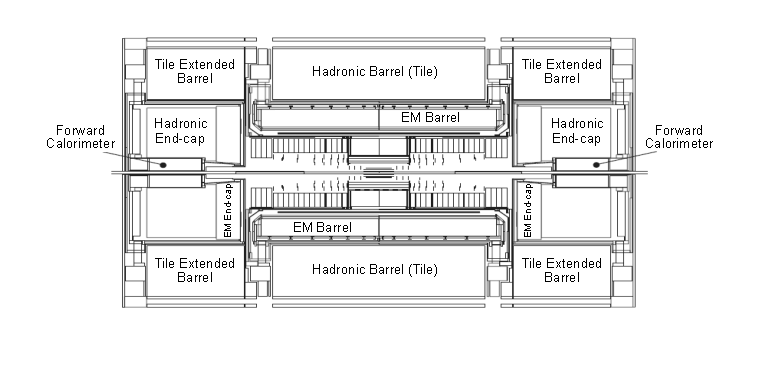
\includegraphics[width=\largefigwidth]{chapters/detector/ATLASCalorimetersFlat.eps}
  \caption{Schematic transverse view ($r$-$z$ view) of the calorimeters in the \ATLAS detector~\cite{ATLAS:2008:detector}. A cylindrical coordinate system is used, with the $z$-axis along the proton-beam.}
  \label{fig:detector:atlas_calorimeters_flat}
\end{figure}

High granularity liquid-argon (LAr) electromagnetic (EM) sampling calorimeters cover the range $\absEta < 3.2$.
In the range $\absEta < 1.7$, the hadronic calorimetry is provided by a scintillator-tile calorimeter.
This is separated into a large central barrel and two smaller extended barrel cylinders, one on either side of the main barrel.
In the end-caps, $\absEta > 1.5$, LAr technology is again used for the hadronic calorimeters, matching the outer \absEta limits of the end-cap electromagnetic calorimeters.
The LAr forward calorimeters extend out to $\absEta = 4.9$, providing both electromagnetic and hadronic energy measurements.

For the inner detector, $\absEta<2.5$, the EM calorimeter is fine-grained to allow precision measurements of electrons and photons to be made.
The other calorimeters in this region are coarser grained, although still possess sufficient resolution to satisfy the physics requirements for jet reconstruction and measurement of \ETmiss.

Calorimeter depth is an important design consideration: the calorimeters must contain electromagnetic and hadronic showers and limit punch-through into the muon system.
Electromagnetic showers are characterised by their narrow lateral profiles and are longitudinally parameterised by their radiation length $X_0$.
Hadronic showers usually have a larger transverse spread and their nuclear interaction length, $\lambda$, is typically an order of magnitude greater than $X_0$, although this is material-dependent.

The barrel of the EM calorimeter is more than \unit{22}{X_0} thick, while the thickness of the end-cap is more than \unit{24}{X_0}.
For high energy jets, the active calorimeter comprises \unit{9.7}{\lambda} in the barrel and \unit{10}{\lambda} in the end-caps; providing adequate resolution.
\FigureRef{fig:detector:deadMaterial} shows the total amount of material, including non-instrumented sections, in units of $\lambda$, as a function of \absEta.
Taking all of this into account, the total thickness, as demonstrated using test beams, is sufficient to reduce punch-through below the level of prompt or decay muons.
Together with the large \pseudorap coverage, this also ensures a good \ETmiss measurement, which is a particularly important signature for those analyses looking for evidence of supersymmetry. 

\begin{figure}[htpb]
  \includegraphics[width=\largefigwidth]{chapters/detector/deadMaterial.eps}
  \caption{Cumulative amount of material in the \ATLAS detector, in units of interaction length, $\lambda$, as a function of \absEta. The coverage from each individual calorimeter component is shown separately, while the sections closest to the interaction point, which are not instrumented for calorimetry, are shown in brown~\cite{ATLAS:2008:detector}.}
  \label{fig:detector:deadMaterial}
\end{figure}

\subsection{Liquid Argon Electromagnetic Calorimeter}
The electromagnetic calorimeter barrel, $\absEta < 1.475$, and end-caps, $1.375 < \absEta < 3.2$, are each housed in their own cryostat.
The central solenoid, located in front of the electromagnetic calorimeter, is a significant source of dead material - approximately \unit{1}{\lambda} at its greatest extent, restricting the maximal achievable calorimeter performance.
Placing the solenoid and the liquid argon calorimeter inside a single vacuum vessel mitigates this effect by eliminating two vacuum walls which would otherwise be required.
The barrel calorimeter consists of two identical half-barrels, separated by a \unit{4}{\milli\metre} gap at $\pseudorap = 0$.
The two end-cap calorimeters are each subdivided into two coaxial wheels: the outer wheel covering the region $1.375 \leq \absEta < 2.5$ and the inner wheel $2.5 \leq \absEta < 3.2$.

The electromagnetic calorimeter is a lead-LAr detector with lead absorber plates along its full coverage and readout provided by accordion shaped electrodes.
This accordion geometry avoids the necessity for azimuthal cracks, providing complete symmetry in $\phi$.
For $\absEta < 2.5$, the region instrumented for precision physics, the calorimeter is segmented in depth into three longitudinal layers, numbered from 1 to 3 outwards from the beam axis.
Outside this region, the end-cap inner wheel is divided into only two sections in depth and also has a coarser lateral granularity.

A presampling detector is installed for $\absEta < 1.8$ in order to allow the energy lost by electrons and photons upstream of the calorimeter to be measured and corrected for.
This consists of an active LAr layer which is \unit{1.1}{\centi\metre} thick in the barrel region, and \unit{0.5}{\centi\metre} thick in the end-cap.

\subsection{Hadronic Calorimeters}
\subsubsection{Tile Calorimeter}
As can be seen in \FigureRef{fig:detector:atlas_calorimeters_flat}, the tile
calorimeter is located outside the electromagnetic calorimeter, extending radially from
\unit{2.28}{\metre} to \unit{4.25}{\metre}. It is a sampling calorimeter,
consisting of steel absorbing plates interleaved with scintillating tiles, which provide the
active material. The hadronic barrel covers $\absEta < 1.0$ and is complemented
by two extended barrels covering $0.8 \leq \absEta < 1.7$; each of these
subdetectors is divided azimuthally into 64 modules in $\phi$.

Similarly to the electromagnetic calorimeter, the tile is segmented into three layers:
approximately 1.5, 4.1 and \unit{1.8}{\lambda} thick for the barrel and 1.5,
2.6 and \unit{3.3}{\lambda} thick in the extended barrel. Two sides of the
scintillating tiles are read out by wavelength shifting fibres into two separate
photomultiplier tubes. The readout cells, built by grouping fibres together in the
photomultipliers, are pseudo-projective towards the interaction region.

\subsubsection{Liquid Argon Hadronic End-cap Calorimeter}
The Hadronic End-cap Calorimeter (HEC) is a copper detector consisting of two
independent wheels per end-cap, located directly behind the end-cap
electromagnetic calorimeter (\FigureRef{fig:detector:atlas_calorimeters_flat})
and sharing the same LAr cryostats. The HEC covers the region $1.5 \leq \absEta < 3.2$,
overlapping with both the tile calorimeter and the forward calorimeter.

Each of the HEC wheels, which span $0.475 \leq r < \unit{2.03}{\metre}$,
is divided into 32 identical wedges in $\phi$ and two segments in depth, giving
four layers per end-cap in total. The wheels closest to the interaction point
are built from \unit{25}{\milli\metre} parallel copper plates, while those
further away use \unit{50}{\milli\metre} copper plates: in each case the first
of these plates is half-thickness. As the HEC is a sampling calorimeter, the copper plates
are interleaved with \unit{8.5}{\milli\metre} gaps filled with liquid argon,
which provides the active medium.

\subsection{Liquid Argon Forward Calorimeter}
The Forward Calorimeter (FCAL) consists of one module at either end of the
detector, approximately \unit{10}{\lambda} deep, providing coverage for the
region $3.2 \leq \absEta < 4.9$. It is integrated into the end-cap cryostats
although recessed by about \unit{1.2}{\metre} from the electromagnetic calorimeter;
because of the limited available depth a high-density design is required. The two
FCALs each contain three modules: a copper calorimeter, optimised for electromagnetic
measurements, and two tungsten calorimeters, predominantly aiming to perform
hadronic measurements. Each module has the form of a matrix, with regularly
spaced longitudinal channels filled with concentric tubes, parallel to the beam
axis. Each tube contains a rod, and is otherwise filled with liquid argon which
acts as the sensitive medium.

\section{Detector Performance}
\subsection{Single Hadron Detector Response}
\label{sec:detector:single-particle}
The response of the calorimeters to isolated charged hadrons can be examined by
considering the ratio of the energy, $E$, deposited in the calorimeter to the momentum,
$p$, of the associated track. Comparing the \angles{E/p} distribution in data and
\MC allows an evaluation to be made of the modelling uncertainty on the calorimeter
response in \MC. \FigureRef{fig:detector:single-particle-response} shows
\angles{E/p} as a function of track momentum for two different bins in \absEta,
after background subtraction. The agreement between data and \MC simulation is
within $\sim2\%$ for particles with momenta in the \unit{1-10}{\GeV} range, increasing
to around 5\% for momenta in the \unit{10-30}{\GeV} range.

\begin{figure}[htpb]
  \subfloat[$\absEta < 0.6$]{
    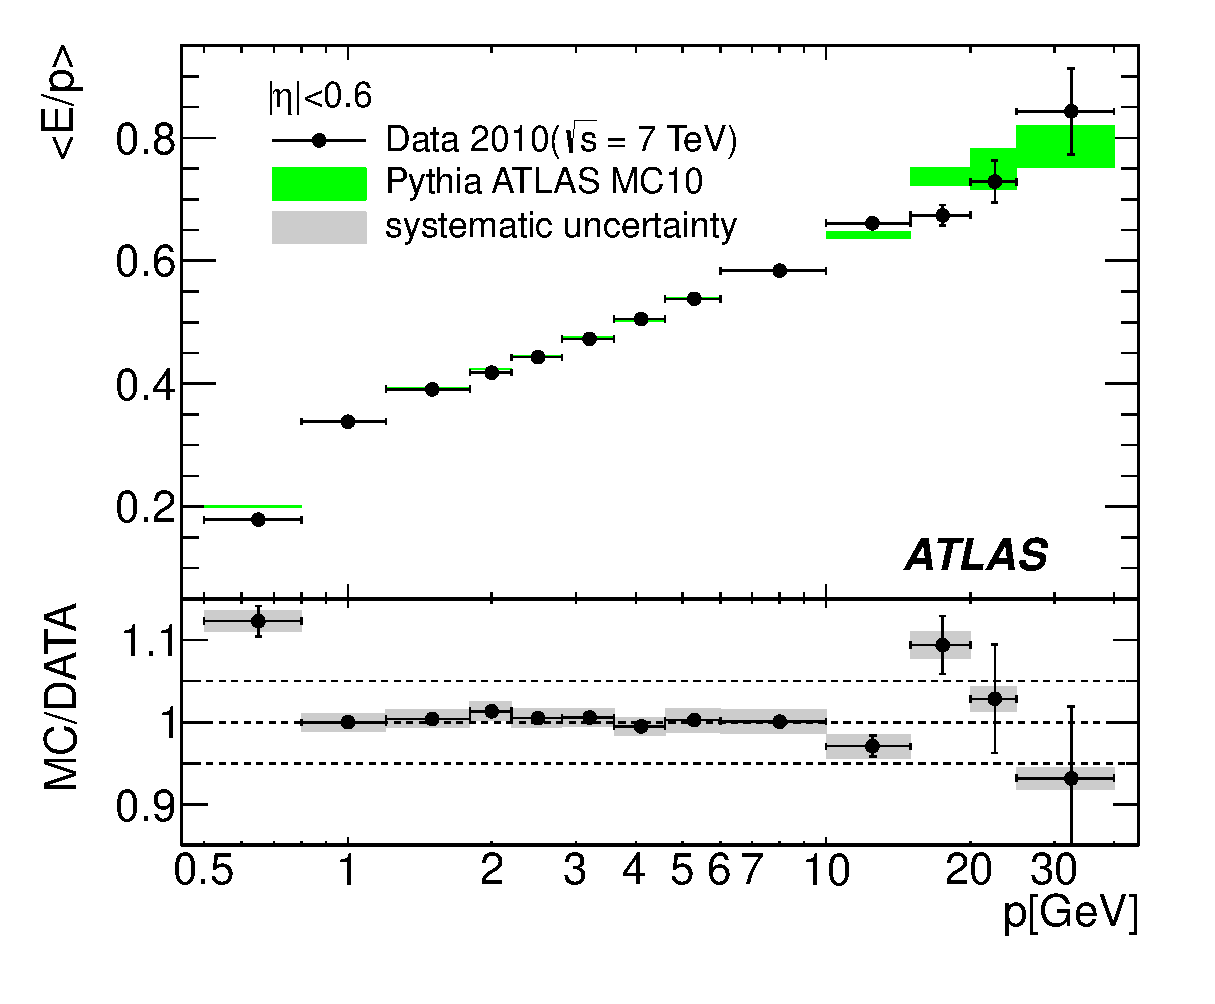
\includegraphics[width=\smallfigwidth]{chapters/detector/SingleParticleEoverP.7TeV.eta0.6.eps}
    \label{fig:detector:single-particle-response_central}}
  \quad
  \subfloat[$0.6 \leq \absEta < 1.1$]{
    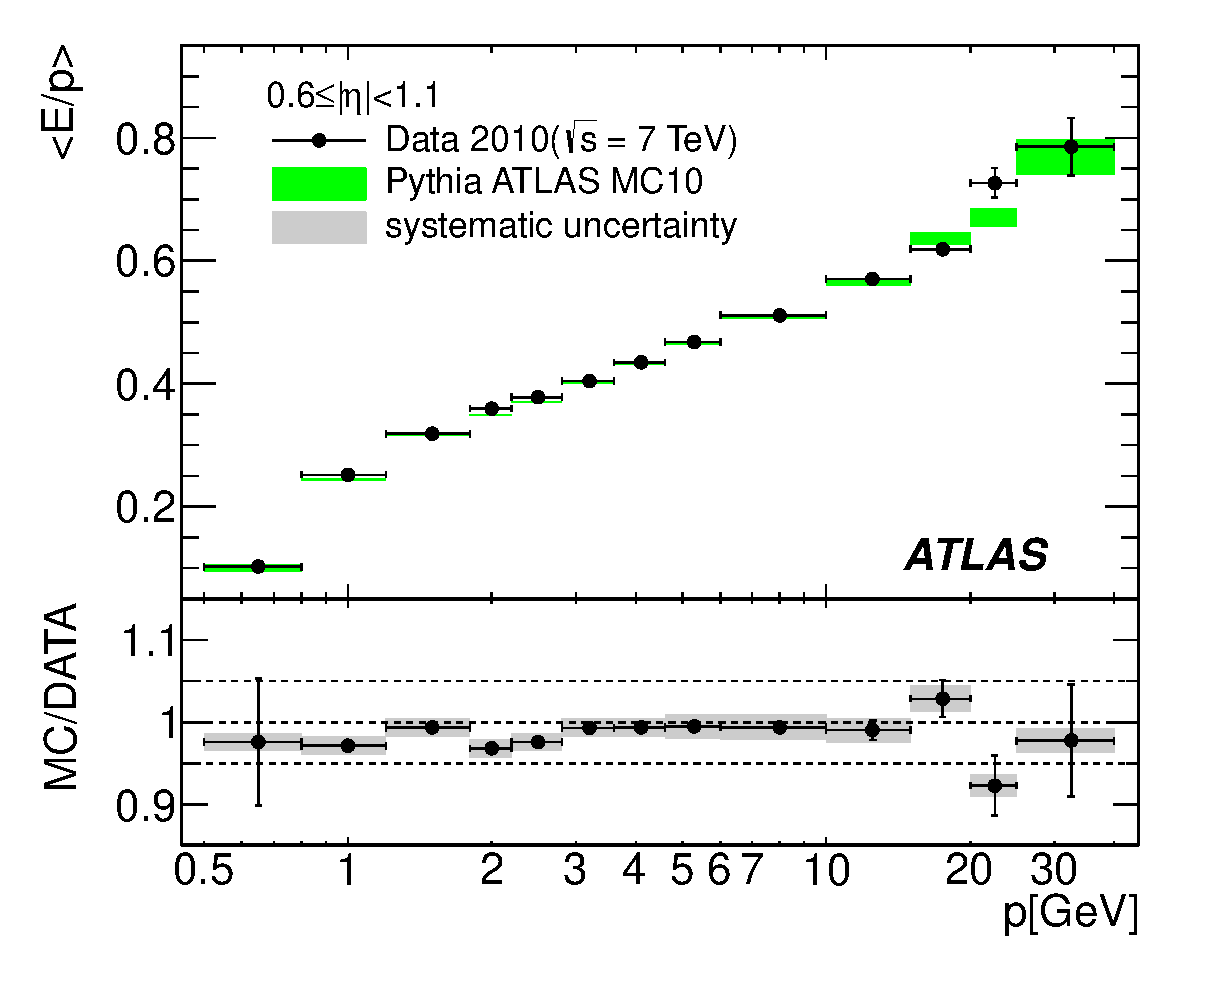
\includegraphics[width=\smallfigwidth]{chapters/detector/SingleParticleEoverP.7TeV.0.6eta1.1.eps}
    \label{fig:detector:single-particle-response_forward}}
  \caption{\angles{E/p} as a function of the track momentum for \protect\subref{fig:detector:single-particle-response_central} central and \protect\subref{fig:detector:single-particle-response_forward} more forward tracks. The black markers represent $\rootS = \unit{7}{\TeV}$ collision data, while the green rectangles show the \MC prediction, with the vertical width indicating the associated statistical uncertainty. The lower sections show the ratio of the \MC simulation prediction to collision data. The grey band indicates the size of the systematic uncertainty on the measurement~\cite{CERN-PH-EP-2012-005}.}
  \label{fig:detector:single-particle-response}
\end{figure}

\subsection{Jet Energy Resolution}
\label{sec:detector:jer}
Fully calibrated jets, see \SectionRef{sec:analysis-tools:jet_reconstruction} for
details, reconstructed using the \akt algorithm with $R=0.6$ are used to study
the jet resolution. Two different methods are used here: the first coming from \dijet
\pT balancing and the second from constructing quantities parallel and transverse
to the \dijet system, known as the bisector technique. For jets with $\absRap < 2.8$,
the results from these two methods are found to be consistent in both data and \MC. 

\begin{figure}[htpb]
  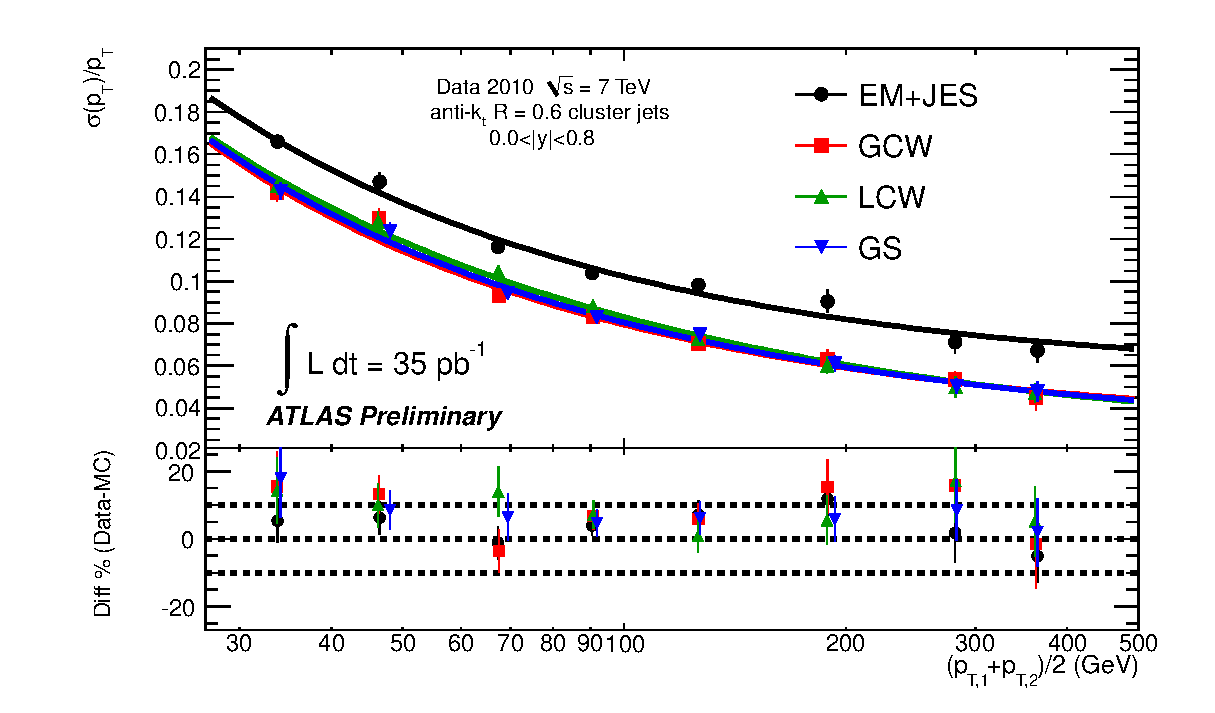
\includegraphics[width=\largefigwidth]{chapters/detector/JERDiffJESDataMC.0.6.eps}
  \caption{Fractional jet energy resolution as a function of average \dijet \pT
           for four different jet calibration schemes: the EM+JES, Global Cell Weighting
           (GCW), Local Cluster Weighting (LCW) and Global Sequential (GS) calibrations;
           only EM+JES has been fully validated for use in \ATLAS, although other
           calibration schemes may be used in future data taking. Lines of best
           fit are shown in each case. The lower section shows the relative difference
           between \MC and the results from data. The black dotted lines indicate
           a relative uncertainty of $\pm10\%$~\cite{ATLAS-CONF-2010-054}.}
  \label{fig:detector:jer}
\end{figure}

\FigureRef{fig:detector:jer} shows the fractional jet energy resolution as
a function of the average \pT of the \dijet system.  The calorimeter jet reconstruction
and selection efficiency relative to track jets is determined in data and \MC using
a tag and probe technique and found to be in good agreement, within systematic uncertainties,
for track jets with \pT values between 5 and \unit{40}{\GeV}~\cite{ATLAS-CONF-2010-054}.

\section{Trigger System}
\label{sec:detector:trigger}
When the design bunch spacing is reached, with collisions occurring every
\unit{25}{\nano\second}, the event rate of \unit{40}{\mega\Hz} is five orders of
magnitude greater than the rate at which data can be recorded, which is limited to 
\unit{400}{\Hz}. This means that the trigger systems must achieve an overall
rejection factor of $10^5$ while avoiding biases and retaining the highest
possible proportion of interesting events. During 2010, the bunch spacing was
kept at \unit{50}{\nano\second}, slightly easing this pressure.

The \ATLAS trigger system has three distinct levels: Level-1 (L1), Level-2 (L2),
and the event filter (EF). Each level of the trigger refines the decision made
by previous levels by applying additional, stricter selection criteria.
Initially, event information is accepted from the readout electronics and
buffered; the hardware-based L1 trigger system then uses a subset of the
available detector information to reject events: budgeting \unit{2.5}{\milli\second}
of processing time per event, it is able to reduce the overall rate to
\unit{75}{\kHz}. Events which pass the L1 trigger are then transferred to the L2
and EF trigger systems, collectively known as the high-level trigger (HLT). Each
HLT trigger is seeded from a specific lower level trigger and is able to examine
relevant features of the event in greater detail in order to make an overall
trigger decision. Events passing one or more triggers after the final,
``Physics'' decision are passed to the data acquisition system.

The central trigger processor implements a `trigger menu', comprising a list of
trigger selections together with their associated prescales; only triggers specified by
the processor are allowed to run in each event. The majority of trigger
menu items are prescaled: only recording a set proportion of otherwise acceptable
events. This allows optimal use of available bandwidth in the face of changing
luminosity conditions.

\subsection{Level-1 Trigger}
Due to the limited time available, the L1 trigger only uses a small amount of
the available detector information: namely the calorimeter and muon systems. The
aim of the L1 system is to identify high \pT leptons, photons and jets as well as events
with large \ETmiss or \ETtotal. High \pT muons are identified using trigger
chambers in the barrel and end-cap regions of the muon spectrometer, while the
identification of other interesting event features is based on reduced-granularity information from all parts of the
calorimeter system. Events which pass the L1 trigger selection are transferred to
the L2 processing system and, if accepted by the HLT, onwards to the
data acquisition systems via point-to-point links.

In each event, the L1 trigger also defines one or more Regions-of-Interest (RoIs):
the geographical coordinates in \etaphi space of those regions within the
detector where its selection process has identified interesting features. The
RoI data includes information on the type of feature identified and the criteria
passed, usually some sort of threshold. This information is passed to the HLT
for later use.

\subsection{High-Level Trigger}
The RoI information from L1 is used to seed the L2 trigger. L2 triggers are able
to use all of the available detector data in the region covered by the RoIs at
full granularity and precision; this corresponds to approximately 2\% of the
total event data. An average event processing time of \unit{40}{\milli\second}
is allowed at this stage, resulting in an output event rate of approximately
\unit{3.5}{\kHz}. The event filter performs the final stage of event selection,
implementing analysis procedures similar to those performed offline to reduce
the final event rate to roughly \unit{400}{\Hz}. In particular, EF jet triggers
implement the \akt algorithm, although this was not used to reject events during
2010.

\subsection{Jet Triggers}
Although the spectrum of jets produced is steeply falling, it would be
preferable from the point of view of physics analyses, particularly differential
cross-section measurements, to have a roughly uniform rate across the full jet
\ET spectrum. Collecting sufficient statistics across the spectrum is also
important for the measurement of detector and trigger efficiencies. Accordingly,
a series of inclusive jet triggers are used, each with a higher threshold than
the previous one. By changing the prescales of these triggers, the jet trigger
menu can be optimised to achieve a roughly flat event rate across the \ET
spectrum despite rising luminosity. The jet-trigger thresholds can also be
changed, but this is a less frequent operation.

The jet trigger is split into logically independent systems: one covering the
central region, $0 \leq \absEta < 3.2$ and one covering the forward region,
$3.2 \leq \absEta <4.9$. At Level-1, these systems use information from
different calorimeter subsystems: central trigger jets rely on information from
the electromagnetic barrel, tile and end-cap calorimeters, while forward trigger
jets use information from the forward calorimeters only. At Level-2, however, information
from multiple trigger systems may be considered, depending on the position of the
L1 RoI, while in the Event Filter, information from the whole detector is
combined~\cite{ATLAS-CONF-2010-028}.

Additionally, the Minimum Bias Trigger Scintillators (MBTS), located in front of
the end-cap cryostats and covering $2.09 \leq \absEta < 3.84$, are often used in jet-based
analyses to provide fully efficient triggering for low \pT jets. The trigger
L1\_MBTS\_1, requiring at least one hit in the minimum bias scintillators, is
the primary trigger used to select minimum-bias events in \ATLAS.

\subsection{Measurements of Trigger Efficiency from Data}
Understanding the efficiencies of relevant triggers is an important part of any
physics analysis. As little weight as possible needs to be given to techniques
relying solely on performance in \MC models; in-situ methods are much preferred.

The two major in-situ methods are the ``orthogonality'' and ``bootstrap''
methods. In each case, these rely on constructing a sample of events which can
then be examined to see what proportion of them pass the trigger of interest.
Orthogonality relies on taking events that pass a trigger which is known to be
uncorrelated to the trigger under consideration. This can, however, introduce physics
biases: muon triggers, for instance, could increase the proportion of
heavy flavour jets. Jet trigger efficiencies are therefore usually determined
using the bootstrap method in which events passing a lower threshold jet trigger,
which is known to be on plateau in the \pT region of interest, are used. Firstly,
events which pass minimum-bias triggers are used to measure the efficiency of
those triggers with the lowest \pT thresholds, then the low threshold jet
triggers are used as the baseline to select events with which to examine higher
\pT-threshold triggers.

Efficiencies can be determined either on a \emph{per-jet} or, more commonly, on
a \emph{per-event} basis. Per-event efficiencies are the fraction of events in
which at least one jet passes the appropriate trigger among all events with at
least one jet at the given \pT. Per-jet efficiencies are the fraction of jets
passing the appropriate trigger among all jets at the given \pT. Per-jet
efficiencies are more complex, due to their reliance on matching between offline
jets and trigger objects and are rarely used.

\FigureRef{fig:detector:forward_bin_trigger_efficiencies} shows per-event
trigger efficiencies for six different triggers in the region $3.6 \leq \absRap < 4.4$.
Here the characteristic serpentine shape of a typical efficiency curve can be seen, rising from zero efficiency to reach a plateau.
In \FigureRef{fig:detector:forward_bin_triggers_L1_akt4}~and~\ref{fig:detector:forward_bin_triggers_L1_akt6}
the efficiencies for L1 triggers are shown. The likelihood that a given L1
trigger will fire, before prescale, is shown as a function of offline jet \pT,
using \akt jets, with $R=0.4$ on the left and $R=0.6$ on the right. Three
different L1 thresholds are shown, each requiring a greater level of L1 \ETEM in
order to trigger. The efficiency for the lowest threshold, L1 $\ETEM > \unit{10}{\GeV}$,
must be determined using MBTS triggers, but higher thresholds can be
bootstrapped from previous jet triggers.

In \FigureRef{fig:detector:forward_bin_triggers_L1L2_akt4}~and~\ref{fig:detector:forward_bin_triggers_L1L2_akt6},
the efficiency curves for L2 triggers are shown, again as a function of offline
jet \pT. The correlation between the \ETEM threshold and the offline \pT at
which plateau is first reached is evident, as is the distinctive shape with
which efficiency rises as a function of offline \pT. Specific details relevant
to the efficiency curves shown here are discussed further in \SectionRef{sec:forward-inclusive:trigger_efficiencies}.

\begin{figure}[htpb]
  \subfloat[L1 efficiency, \akt $R=0.4$ jets]{
    \includegraphics[width=\smallfigwidth]{chapters/forward-inclusive/forward_bin_triggers_L1_akt4.eps}
    \label{fig:detector:forward_bin_triggers_L1_akt4}}
  \quad
  \subfloat[L1 efficiency, \akt $R=0.6$ jets]{
    \includegraphics[width=\smallfigwidth]{chapters/forward-inclusive/forward_bin_triggers_L1_akt6.eps}
    \label{fig:detector:forward_bin_triggers_L1_akt6}}
  \\
  \subfloat[L1+L2 efficiency, \akt $R=0.4$ jets]{
    \includegraphics[width=\smallfigwidth]{chapters/forward-inclusive/forward_bin_triggers_L1L2_akt4.eps}
    \label{fig:detector:forward_bin_triggers_L1L2_akt4}}
  \quad
  \subfloat[L1+L2 efficiency, \akt $R=0.6$ jets]{
    \includegraphics[width=\smallfigwidth]{chapters/forward-inclusive/forward_bin_triggers_L1L2_akt6.eps}
    \label{fig:detector:forward_bin_triggers_L1L2_akt6}}
  \caption{Jet trigger efficiency at L1 (top) and combined L1+L2 (bottom) as a function of
           reconstructed jet \pT for \akt jets with $R=0.4$ (left) and $R=0.6$ (right) in the
           forward region $3.6 \leq \absRap < 4.4$, shown for three different trigger thresholds in each case.
           The trigger thresholds are at the electromagnetic scale, while the jet \pT is at the
           calibrated scale (see \SectionRef{sec:analysis-tools:jet_reconstruction}). Due
           to the presence of a dead FCAL trigger tower, which spans 0.9\% of the
           \etaphi acceptance, the efficiency is not expected to reach 100\%.}
  \label{fig:detector:forward_bin_trigger_efficiencies}
\end{figure}

  \chapter{Analysis Tools}
\label{chap:analysis-tools}

\chapterquote{An architect's most useful tools are an eraser at the drafting board, and a wrecking bar at the site.}{Frank Lloyd Wright}

\section{Introduction}
Progressing from raw detector output to final results and distributions, which can be compared to theoretical predictions, involves a series of sequential steps.
The initial steps are generic to any analysis: the rejection of events for data quality reasons, the reconstruction of jets from calorimeter signals and their subsequent calibration are, in general, performed identically for each analysis.
Additionally, unfolding for detector effects, in other words correcting distributions made at detector level back to the final-state particle level, is
often necessary.

\section{Jet Reconstruction and Calibration}
\label{sec:analysis-tools:jet_reconstruction}
The default jet-clustering algorithm in \ATLAS is \akt (see \SectionRef{bg-theory:recombination_algorithms}), implemented using \fastjet~\cite{Cacciari:2005:fastjet,Cacciari:2012:fastjet}, with two different $R$-parameters: narrow jets with $R=0.4$ and wide jets with $R=0.6$.

Jets are reconstructed by applying a jet-clustering algorithm to calorimeter signals, and subsequently performing a calibration step, to correct for known detector effects.
Two different inputs from the calorimeter can be used for jet-finding, towers and topological clusters.

Towers are formed by collecting cells into bins of a regular $\DeltaEta \times \DeltaPhi = 0.1 \times 0.1$ grid, depending on their location, and summing up their signals, or a fraction of their signal corresponding to the overlap area fraction between the tower bin and the relevant cell.
This summing stage is non-discriminatory, in other words all calorimeter cells are used in the towers.
Towers with negative signals are recombined with nearby positive signal towers until the net signal is positive, thus all resulting towers have a valid physical four-vector and can directly be used by the jet finders.
This approach can be understood as an overall noise cancellation rather than suppression, since noisy cells will still contribute to the jets.

Topological cell clusters~\cite{ATLAS-LARG-PUB-2008-002} are an attempt to reconstruct three-dimensional energy depositions in the calorimeter~\cite{Cojocaru:2004:ATLASHadronicCalibration,Andrieu:1993:H1PionCalibration}.
Firstly, any cell which satisfies $|E_{cell} | > 4\sigma_{cell}$ is identified as a ``seed cell'', where $\sigma$ is the RMS noise of the cell due to electronic effects and pile-up.
Any cell neighbouring a seed cell, which itself satisfies $|E_{cell}| > 2\sigma_{cell}$, is incorporated into the topocluster, and this process is repeated iteratively until there are no longer any cells adjacent to the topocluster with $|E_{cell}| > 2\sigma_{cell}$.
Finally, an outer layer of cells is added, here accepting any surrounding cells which satisfy $E_{cell} > 0$ is added.
Known hot cells or dead cells are excluded from this process.
In contrast to using signal towers, using this 4-2-0 clustering scheme inherently incorporates noise suppression and results in fewer cells being included in the jet clustering step.
In jet reconstruction, each topocluster is considered to be a massless particle with energy $E = \sum{E_{cell}}$ and position given by the energy-weighted centroid of cells in the cluster, with the direction pointing back towards the geometric centre of the detector.

Jets produced in this way are reconstructed at the electromagnetic (EM) scale, which is the basic signal scale for the \ATLAS calorimeters. It accounts
correctly for the energy deposited in the calorimeter by electromagnetic showers - validated using test-beam measurements with electrons and muons.
It does not, however, correct for the lower hadron response, and a series of calibration steps is therefore needed to bring an uncalibrated, EM-scale jet to the hadronic scale energy scale~\cite{ATLAS-CONF-2010-056,CERN-PH-EP-2011-191}.
Jets which fall below the reconstruction threshold of \unit{7}{\GeV} are discarded before calibration.

\subsection{Pile-up Correction}
\label{sec:analysis-tools:pileup_correction}
Jets calibrated at the EM-scale are affected by energy deposits arising from multiple proton-proton interactions within the same bunch crossing, known as
pile-up.
Pile-up can be either out-of-time, in other words, occurring slightly before or after the hard interaction or in-time, occurring contemporaneously.
The \ATLAS calorimeter response is such that the time integral of the signal corresponding to a single particle is zero: in other words a sharp positive peak is followed by a longer but lower amplitude trough.
This ensures that the calorimeter is not saturated when large numbers of particles arrive in close succession but also means that, while in-time pile-up provides a positive contribution to the calorimeter signal, out-of-time pile-up will provide negative contribution.
A correction to remove the average effects of these additional proton-proton interactions, derived using minimum bias data, is applied at the electromagnetic scale: the average additional \ET per calorimeter tower, measured as a function of \pseudorap and the number of reconstructed primary vertices $N_{PV}$, is subtracted from each jet.

\subsection{Jet Origin Correction}
The calorimeter clusters used for jet reconstruction are assumed to originate from the geometrical centre of ATLAS.
The jet origin correction first corrects each calorimeter cluster to instead point back to the primary vertex with the highest $\sum{\pT^{track}}$ of the event; the beam spot is used if there is no primary vertex.

The kinematics of each calorimeter cluster are recalculated using the direction from the primary vertex to the centroid of the cluster.
The raw jet four momentum is then redefined as the four vector sum of the clusters.
This correction improves the angular resolution while the jet energy is unaffected.
A small improvement in jet \pT resolution is introduced due to the changing jet direction, although this is rarely larger than 1\%.
Most of the effect of the correction comes from the $z$-position of the primary vertex.

\subsection{Final Jet Energy Scale}
\label{sec:analysis-tools:final_JES}
The final part of the jet calibration involves applying a jet energy scale (JES) correction to account for the fact that the jets are reconstructed at the
electromagnetic (EM) scale.
This is known as the EM+JES calibration, and it corrects for  calorimeter non-compensation, energy losses in inactive regions, out-of-cone showering effects as well as inefficiencies in the calorimeter clustering and jet reconstruction.
This calibration is primarily dependent on energy, since the calorimeter response is energy-dependent, and the jet direction, due to the changing calorimeter technology and to the varying amounts of dead material in front of the calorimeters.

The EM+JES calibration is derived from simulated events, specifically the AMBT1 \Pythia \dijet sample.
To derive the correction factors in \MC, isolated particle jets, reconstructed using final-state particles, are matched with isolated detector level jets, reconstructed using the full calorimeter level information.
The particle jet energy is then divided by the EM-scale energy of the matching calorimeter jet in order to obtain the appropriate correction factor.

Following this, a small \pseudorap-dependent correction is applied to remove a bias in the reconstructed \pseudorap of jets that occurs when jets fall in poorly instrumented regions of the calorimeter that have a lower response than the regions around it.
The reconstructed direction of the jet will be biased since the clusters that fall in these regions have a lower response when their four-vectors are added up to build the jet four-vector, and hence a smaller overall weight.
As a consequence of this, the jet is pulled toward the region with the higher response.
This \pseudorap-correction is parameterized as a function of jet energy and pseudorapidity, and is small, $\DeltaEta < 0.01$, in most regions of the calorimeter, although larger in the crack regions: up to $\DeltaEta = 0.07$ for low \pT jets in the HEC-FCAL transition region.

\section{Generic Event Selection Considerations}
\label{sec:analysis-tools:data_selection}
\subsection{Luminosity}
All of the studies presented in this thesis were carried out at a centre-of-mass
energy of \rootS = \unit{7}{\TeV} using the \twentytenlumi of integrated
luminosity that was collected during 2010 (see \FigureRef{fig:analysis-tools:luminosity}).

The luminosity was measured independently by multiple detectors and algorithms,
each of which had differing acceptances, systematic uncertainties and background 
sensitivities. In 2010, the primary methods used were LUCID, a dedicated \v{C}erenkov
detector and counting hits in the MBTS. For both of these, the case in which hits
were registered on the A-side AND the C-side of the detector was treated as a separate
measurement from the case in which the requirement was only for a hit on at least
one of these.

\begin{figure}[htpb]
  \subfloat[2010 luminosity evolution]{
    \includegraphics[width=\smallfigwidth]{chapters/analysis-tools/sum2010LumiByDay.eps}
    \label{fig:analysis-tools:luminosity_nonLog}}
  \quad
  \subfloat[2010 luminosity evolution, logarithmic scale]{
    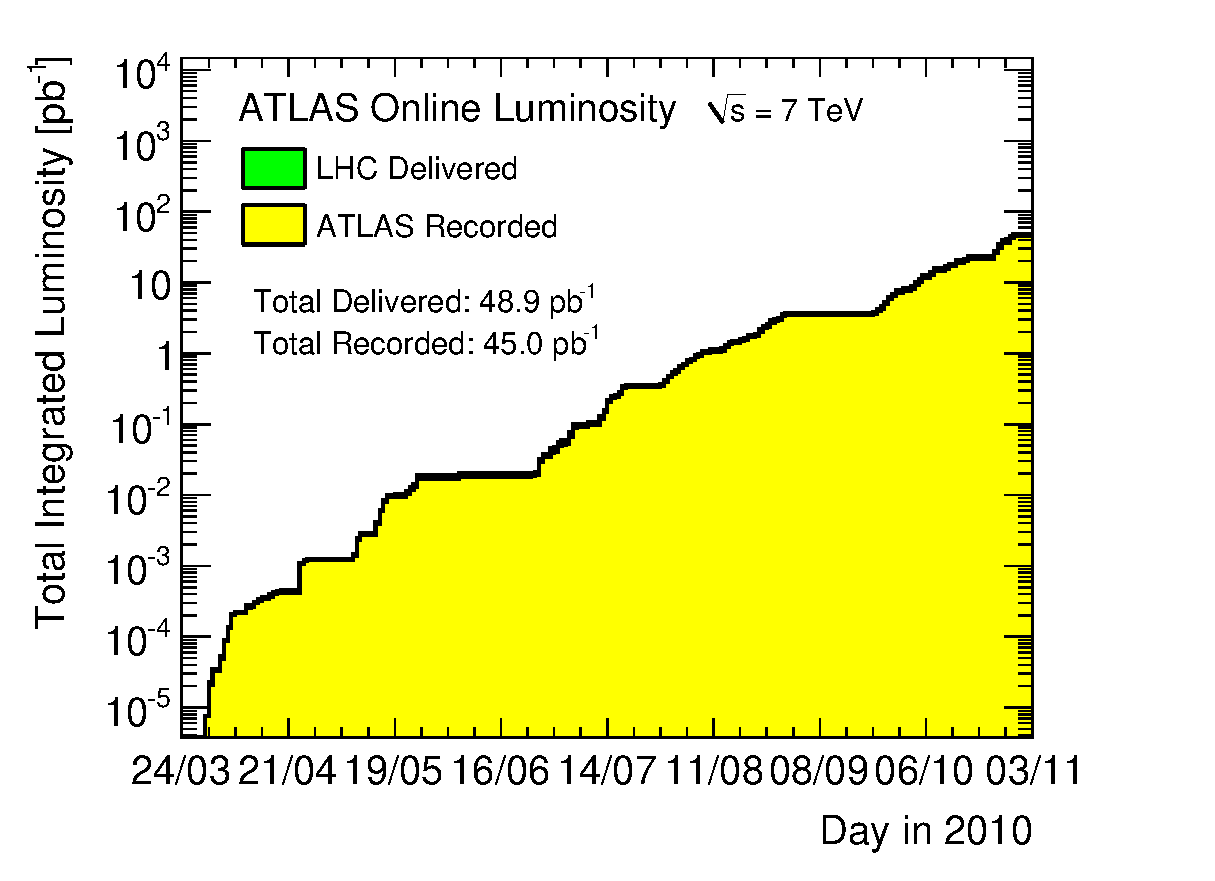
\includegraphics[width=\smallfigwidth]{chapters/analysis-tools/sum2010LumiByDayLog.eps}
    \label{fig:analysis-tools:luminosity_log}}
  \caption{Total integrated luminosity available in \ATLAS and recorded by the \LHC in 2010. Identical information is shown in \protect\subref{fig:analysis-tools:luminosity_nonLog} and \protect\subref{fig:analysis-tools:luminosity_log}, with the only difference being that a logarithmic scale is used in the latter case~\cite{ATLAS-CONF-2011-011}.}
  \label{fig:analysis-tools:luminosity}
\end{figure}

The van der Meer method discussed in \SectionRef{sec:bg-theory:luminosity} was used
to obtain $\sigma_{vis}$ for each of these processes. The differences between the
luminosities obtained from each method were monitored as a function of time
and of $\mu$. The measurements were finally combined to produce the overall \ATLAS
luminosity determination, together with its uncertainty~\cite{CERN-PH-EP-2010-069}.

A single run of proton-proton collisions is divided into luminosity blocks, each of
which typically represents about two minutes of data taking, within which
conditions such as bunch spacing and beam intensity are constant. The
instantaneous luminosity, bunch size and bunch shaping each evolved over the
course of this period of data taking; data collected in \ATLAS is therefore divided
into different run periods, with the boundaries of these periods being defined by
changes in running conditions. The dates and total integrated luminosity corresponding
to each of these run periods are summarised in \TableRef{tab:analysis-tools:luminosity-periods}.

\begin{table}
\begin{center}
  \begin{tabular}{ c@{\hskip 1cm} c c c c c }
    Period                         &   A    &   B    &   C    &   D    &   E    \\
    Start of data taking           & Mar 30 & Apr 23 & May 18 & Jun 24 & Jul 29 \\
    End of data taking             & Apr 19 & May 17 & Jun 05 & Jul 18 & Aug 17 \\
    Luminosity [$\nano\barn^{-1}$] & 0.380  & 8.07   & 8.46   & 201    & 1000   \\
    \cmidrule{2-6}
    Period                         &   E5   &   F    &   G    &   H    &  I     \\
    Start of data taking           & Aug 10 & Aug 19 & Sep 22 & Oct 08 & Oct 24 \\
    End of data taking             & Aug 17 & Aug 30 & Oct 06 & Oct 18 & Oct 29 \\
    Luminosity [$\nano\barn^{-1}$] & 445    & 1810   & 6870   & 7250   & 19100  \\
  \end{tabular}
  \caption{Dates and total integrated luminosity for each of the nine data taking periods for data collected by \ATLAS in 2010. Separate numbers are presented for period E and period E5 (which excludes the first four sets of runs in this period) due to a software problem which affected forward jet triggers at this time.}
  \label{tab:analysis-tools:luminosity-periods}
\end{center}
\end{table}

\subsection{Data Quality}
Certain generic cuts, held in common between all analyses are necessary in order
to extract useful events from the recorded data. First, the event is required to
belong to one of a set of ``good runs''. These are specific luminosity blocks in
which the relevant detector subsystems, trigger and reconstructed physics
objects have passed a data-quality assessment and are deemed suitable for
physics analysis. For the analyses discussed in this thesis, this means the
central trigger processor, solenoid magnet, inner detectors (Pixel, SCT, and
TRT), calorimeters (barrel, end-cap, and forward) and the luminosity recording
system.

\subsection{Primary Vertex}
To reject events arising from cosmic-ray muons and other non-collision backgrounds,
events are selected as collision candidates by requiring that they have at
least one primary vertex that is consistent with the beamspot position and that
has at least five tracks associated to it, each with $\pT > \unit{0.5}{\GeV}$.
This vertex definition is consistent with that used to evaluate pile-up vertices
in the offset correction, as discussed in \SectionRef{sec:analysis-tools:pileup_correction}.
The efficiency for collision events to pass this vertex requirement, although
obviously analysis dependent, is generally well over 99\%.

\subsection{Jet Cleaning}
\label{sec:analysis-tools:jet_cleaning}
Standard jet cleaning criteria have been developed in order to identify fake jets
which arise due to noise or to out-of-time energy depositions. Jets failing these criteria
are flagged as either ``bad'', likely to be fake, or ``ugly'', likely to be
mismeasured due to falling into less well instrumented
regions~\cite{ATLAS-CONF-2010-038,ATLAS-CONF-2010-050}. Three main issues are
addressed, with a dedicated set of selection criteria for each:

\begin{itemize}
  \item \textbf{Single-cell jets in the HEC.} Most misreconstructed jets arise
    from noise bursts in the HEC. This results in jets with most of their energy
    coming from single calorimeter cells.
  \item \textbf{Bad quality jets in the EM calorimeter.} Noise bursts in the
    EM calorimeter, although rarer than in the HEC, result in jets with most of
    their energy coming from the EM calorimeter and whose cells have bad
    reconstruction ``quality\footnote{$Q$-factor, one of the inputs to jet cleaning,
                                      is a measure of the quality of the signal
                                      in a given LAr cell, analogous to $\chi^2$,
                                      parameterising how well the expected pulse
                                      shape fits the digitised samples and thus
                                      how well the amplitude is measured in this
                                      cell. Cutting on this variable aims to remove
                                      large but badly measured cell amplitudes which
                                      could otherwise fake a jet.}''.
  \item \textbf{Out-of-time jets.} When large out-of-time energy deposits appear
    in the calorimeter, possibly from photons produced by cosmic rays, jets will
    be reconstructed with timing that is incompatible with the event time.
\end{itemize}

A series of per-jet variables, seen in \TableRef{tab:analysis-tools:jet_cleaning_variables}
are used to reject jets falling into one of these categories.

\begin{table}
\begin{center}
  \begin{tabular}{ c l }
  EMf        & fraction of energy coming from the EM calorimeter                             \\
  FMax       & maximum energy fraction in one calorimeter layer                              \\
  HECf       & energy fraction in the HEC                                                    \\
  LArQ       & the fraction of energy coming from LAr cells having $Q$-factor $>4000$        \\
  HECQ       & same as the LArQuality except calculated only with the HEC                    \\
  NegE       & negative energy in the jet                                                    \\
  t          & the mean timing difference between cells in the jet and the event time        \\
  \pseudorap & \pseudorap at the EM-scale                                                    \\
  Chf        & the ratio of the $\sum{\pT^{track}}$ associated to the jet divided by jet \pT \\
  \end{tabular}
  \caption{Per-jet variables used as an input to jet cleaning.}
  \label{tab:analysis-tools:jet_cleaning_variables}
\end{center}
\end{table}

Three levels of bad jet rejection have been determined by the \ATLAS Jet/Etmiss
Working Group. The most lenient of these is termed ``loose'' cleaning, with
``medium'' and ``tight'' successively applying stricter criteria in identifying
additional jets as bad. The jet cleaning cuts used in each of these cases are
shown in \TableRef{tab:analysis-tools:jet_cleaning}.

\begin{table}
\begin{center}
  \begin{tabular}{ l c c c }
             & Loose                            & Medium = Loose OR             & Tight = Medium OR     \\ 
  \midrule
             & $\text{HECf}>0.5$ \&             &                               &                       \\
  HEC        & $|\text{HECQ}|>0.5$              & $\text{HECf}>1-|\text{HECQ}|$ &                       \\
  spikes     & OR                               &                               &                       \\
             & $|\text{NegE}|>\unit{60}{\GeV}$  &                               &                       \\
  \midrule
             & $\text{EMf}>0.95$ \&             & $\text{EMf}>0.9$ \&           &  $\text{EMf}>0.98$ \& \\
  EM         & $|\text{LArQ}|>0.8$ \&           & $|\text{LArQ}|>0.8$ \&        & $|\text{LArQ}|>0.05$  \\
  coherent   & $|\eta|<2.8$                     & $|\eta|<2.8$                  &                       \\
  noise      &                                  &                               & OR                    \\
             &                                  &                               & $|\text{LArQ}|>0.95$  \\
  \midrule
             & $|t|<\unit{25}{\nano\second}$    & $|t|<\unit{10}{\nano\second}$ &                       \\
             & OR                               & OR                            &                       \\
             & $\text{EMf}<0.05$ \&             & $\text{EMf}<0.05$ \&          & $\text{EMf}<0.1$ \&   \\
  Non-       & $\text{Chf}<0.05$ \&             & $\text{Chf}<0.1$ \&           & $\text{Chf}<0.2$ \&   \\
  collision  & $|\eta|<2$                       & $|\eta|<2$                    & $|\eta|<2$            \\
  background & OR                               & OR                            & OR                    \\
  and        & $\text{EMf}<0.05$ \&             & $\text{EMf}>0.95$ \&          & $\text{EMf}>0.9$ \&   \\
  cosmics    & $|\eta| \geq 2$                  & $\text{Chf}<0.05$ \&          & $\text{Chf}<0.02$ \&  \\
             &                                  & $|\eta|<2$                    & $|\eta|<2$            \\
             & OR                               &                               &                       \\
             & $\text{FMax}>0.99$ \&            &                               & $\text{EMf}<0.1$ \&   \\
             & $|\eta|<2$                       &                               & $|\eta| \geq 2$       \\
  \end{tabular}
  \caption{The cuts used to remove bad jets as part of jet cleaning in \ATLAS.
           Each of the three sets of cuts are shown: loose, medium and tight. A
           jet is considered ``bad'' if it passes any of these cuts. The medium
           cuts comprise the loose cuts plus additional requirements, while the
           tight cuts have the same relationship to the medium cuts. This means
           that any jet considered bad by the loose (medium) cuts will
           automatically be considered bad when using the medium (tight) cuts.}
  \label{tab:analysis-tools:jet_cleaning}
\end{center}
\end{table}

As well as this removal of bad jets, ugly jets are identified as those jets
with more than 50\% of their energy coming either from TileGap3, the transition
region between the barrel and end-cap, or from known dead cells, which are
assigned an energy value based on the values of their neighbouring cells.

\subsection{Jet Energy Scale Uncertainty}
\label{sec:analysis-tools:jes_uncertainty}
As discussed in \SectionRef{sec:analysis-tools:final_JES}, the jet energy scale
(JES) is derived in \MC before being validated using a series of in-situ
measurements. Evaluating the JES uncertainty therefore necessitates combining
uncertainties arising from each of these sources: in-situ and single pion
test-beam measurements, uncertainties on precise details of material
distribution in the \ATLAS detector, the \MC modelling used in event simulation
and electronic noise must all be considered~\cite{ATLAS-CONF-2010-056,CERN-PH-EP-2011-191}.
%The jet energy scale (JES), as discussed in ,
%has multiple sources of systematic uncertainty, Evaluation of the level of
%uncertainty on the JES requires information from each of these sources to be combined:

Important individual sources of uncertainty include: non-closure when the JES
correction is applied to reconstructed \MC; the single particle calorimeter response determined
from in-situ measurements, as described in \SectionRef{sec:detector:single-particle};
the accuracy of detector simulations obtained by varying calorimeter noise in \MC samples; the
uncertainty associated with physics modelling, which is obtained from comparing
the detector response in different \MC generators and finally the  relative
jet calibration obtained through \etaint, as discussed in
\ChapterRef{chap:eta-intercalibration}. The level of JES uncertainty is shown in
\FigureRef{fig:analysis-tools:JESUncertainty} as a function of jet \pT for
central and for forward jets.

\begin{figure}[htpb]
  \subfloat[$0.3 \leq \absEta < 0.8$]{
    \includegraphics[width=\smallfigwidth]{chapters/analysis-tools/JESUncertainty_AntiKt6Topo_EMJES0.3-0.8.eps}
    \label{fig:analysis-tools:JESUncertainty_central}}
  \quad
  \subfloat[$3.6 \leq \absEta < 4.5$]{
    \includegraphics[width=\smallfigwidth]{chapters/analysis-tools/JESUncertainty_AntiKt6Topo_EMJES3.6-4.5.eps}
    \label{fig:analysis-tools:JESUncertainty_forward}}
  \caption{Fractional jet energy scale systematic uncertainty is shown as a
           function of \pT for jets in two pseudorapidity regions: \protect\subref{fig:analysis-tools:JESUncertainty_central}
           $0.3 \leq \absEta < 0.8$ and \protect\subref{fig:analysis-tools:JESUncertainty_forward}
           $3.6 \leq \absEta < 4.5$. In the forward region, the JES uncertainty
           is extrapolated from the barrel uncertainty, with the uncertainty contribution
           from the \etaint between central and forward jets in data and \MC added
           in quadrature. The total uncertainty is shown as the solid light blue
           area. The individual sources are also shown, with uncertainties from
           the fitting procedure where applicable~\cite{ATLAS-CONF-2010-056,CERN-PH-EP-2011-191}.}
  \label{fig:analysis-tools:JESUncertainty}
\end{figure}

\subsection{Jet Trigger Threshold Evolution}
\label{sec:analysis-tools:jet_selection_evolution}
As data conditions have changed over time, the trigger has changed to reflect
this: both through enabling the HLT, which was initially used in passthrough
mode, and by changing trigger prescales to keep the overall recorded event rate
within acceptable bounds. This was primarily done by prescaling triggers with
lower \ET thresholds, while the triggers with the highest \ET thresholds
remained unprescaled.

In general, the aim of jet-based analyses is to retain as high a proportion of events as
possible while minimising the biases and systematic uncertainties arising from
the trigger. The easiest way to achieve this is to use the trigger in the
plateau region where its efficiency is close to 100\%. In order to accept as
many events as possible, hence reducing statistical uncertainty, the trigger
thresholds used in analyses are usually chosen to be the lowest ones for which
trigger efficiency is still larger than 99\%, thus ensuring that the effects of
prescaling are as small as possible.

For high \pT jets in the central region, this means that the trigger of choice
changes over time, as successive triggers become increasingly prescaled. For
low \pT jets, the majority of the recorded data comes from periods A--C, recorded
between March and June 2010, when much of the trigger bandwidth was allocated to
minimum bias triggers. For forward jets, the first four periods (A--D) could not
be used, as the forward jet trigger had not yet been commissioned, so the
majority of analyses can use only periods E--I.

In 2010 only L1 information was used to select events in the early periods, up
until the summer, while L2 was used from the summer to the end of the year. The
jet trigger did not reject events at the EF stage in 2010. In the early part of
Period A, before run 152777, a mistiming in the L1 central jet trigger hardware
caused large inefficiencies although MBTS triggers were not affected by this.
Additionally, further calibration problems mean that forward jet triggers cannot
be used during the early runs of period E.

\section{Unfolding Detector Effects}
\label{sec:analysis-tools:unfolding}
Unfolding is a procedure which attempts to correct distributions made using
information from the detector output back to the equivalent distributions that
would have been seen given an ideal detector which was able to perfectly measure
all final-state particles in the event. Unfolding aims to compensate for
smearing effects in the detector as well as for event selection inefficiencies. This
allows easy comparison to any theoretical calculation even if, at some future
point, the precise details of the detector simulation are lost.

Various different unfolding methods are used in different analyses, but they all
share one essential feature: they rely on comparison, using one or more \MC{s}
generators, between final-state particle level (hadron level) information and
the equivalent information after detector simulation and reconstruction have
been applied (detector level).

Bin-by-bin unfolding relies entirely on the shape of distributions in \MC in order
to compute the correction factors. Firstly, for each relevant distribution, the
ratio between the hadron level and detector level predictions is calculated.
This ratio is then applied as a correction factor to the measured data. This
technique can only be applied when migrations between bins are small in
comparison to the bin contents, often forcing the use of large bins. Efficiency,
the proportion of events which remain in the same bin between hadron level and
detector level, and purity, the proportion of events in a given detector level
bin which were in that bin at hadron level are important in assessing the impact
of inter-bin migrations.

For the Singular Value Decomposition (SVD) method, the first step is to
construct a 2D transfer matrix, providing full information about movements from
one bin to another between hadron level and detector level. A singular value
decomposition is then used in order to prevent fluctuations that a simple
inversion of this transfer matrix would introduce. However, the regularisation
procedure in SVD also uses a constraint on the curvature of the unfolded
spectrum, which introduces long-range correlations in the result that produce an
artificial smoothing of the unfolded distribution and which can also cause
biases.

The Iterative, Dynamically Stabilised (IDS) method uses the same transfer matrix
to compute the matrix of unfolding probabilities, which encodes the probability
for an event reconstructed in a given bin $i$ to be generated in bin $j$. The
unfolding matrix is improved in a series of iterations, where the hadron level \MC is
reweighted to the shape of the corrected data spectrum. The regularisation,
preventing statistical fluctuations from being amplified by the successive
iterations, is provided by the use of the significance of the differences
between data and \MC in each bin. The final unfolding matrix, after the optimal
number of iterations, is used to correct the reconstructed spectrum for detector
effects.

Finally, unfolding based on Bayes' theorem uses the transfer matrix to obtain a
series of transition probabilities: given a certain hadron level result, what are
the probabilities for each detector level measured outcome. Bayes' theorem is then
used to calculate the reverse probability: given a detector level outcome, what
is the probability that the hadron level result could have come from each bin of
the measurement: this process is then repeated iteratively~\cite{DAgostini:2010:BayesianUnfolding}.

  \chapter{\etaint}
\label{chap:eta-intercalibration}

\chapterquote{The best and safest thing is to keep a balance in your life. If
you can do that, and live that way, you are really a wise man.}{Euripides}

\section{Introduction}
As discussed in \SectionRef{sec:detector:calorimeter_systems}, the \ATLAS
calorimeters use different technology in different detector regions, with
varying amounts of dead material in front of the calorimeters. In order to
ensure that the calorimeter response to jets is uniform throughout \etaphi space,
it is therefore necessary to apply a jet-level calibration. This calibration is
determined, at least in part, using \MC samples, however, given the non-compensating nature of the calorimeters
together with the complex calorimeter geometry and material distribution, it is
clear that such corrections need to be validated in-situ. The relative response
of the calorimeter system to jets can be determined by studying the balance of transverse
momenta in \dijet{s}. 

\section{Intercalibration using Events with \Dijet Topologies}
\subsection{Intercalibration using a Central Reference Region}
\label{sec:etaint:central_reference}
In the central region of the calorimeter, it is possible to use tracking information
to reconstruct jets. This entails using ``good'' tracks in the inner detector; those
with \pT > \unit{500}{\MeV}, a transverse impact parameter less than \unit{1.5}{\milli\metre}
from the primary vertex, a longitudinal impact parameter satisfying $|z_0 \sin{\theta}| < \unit{1.5}{\milli\metre}$
and with at least six hits in the SCT. These tracks are then used as input to the
\akt algorithm, with the jets thus obtained being termed track jets. The calibration
of calorimeter jets can be cross-checked using these track jets, in particular by looking for
any systematic differences in their \pT or \pseudorap distributions.

As a result, the standard approach for \etaint with \dijet events is to use the
central region of the barrel, $\absEta < 0.8$, as a reference region.
The relative calorimeter response of jets in other calorimeter regions is
quantified by the \pT balance between the reference jet and the probe jet,
exploiting the fact that, in the absence of any additional radiation in the
event, these jets are expected to have equal \pT due to conservation of
transverse momentum. The \pT balance is characterised by the asymmetry
\Asymmetry, defined as

\begin{equation}
  \Asymmetry = \frac{\pTprobe - \pTref}{\pTavg}
\end{equation}

\noindent with \pTavg = (\pTprobe + \pTref)/2. If both jets fall into the
reference region, each jet is used, in turn, to probe the other. As a
consequence, the average asymmetry in the reference region will be zero by
construction; although this may not be true in the regions $-0.8 \leq \pseudorap < 0$
and $0 \leq \pseudorap < 0.8$ when these are considered individually.

The asymmetry is then used to measure an \etaint factor, \relResponse, for the
probe jet or, conversely, the response of the probe jet relative to the
reference jet, 1/\relResponse, using the relation

\begin{equation}
  \frac{\pTprobe}{\pTref} = \frac{2 + \Asymmetry}{2 - \Asymmetry} = 1 / \relResponse 
\end{equation}

This analysis is performed in bins of jet \pseudorap and \pTavg. Using the
standard method outlined above, there is an asymmetry distribution \Aik for each
probe jet \pseudorap-bin $i$ and each \pTavg-bin $k$. Intercalibration factors
are calculated for each bin according to \EquationRef{eq:etaint:RelResponseRelation}

\begin{equation}
  \relResponse_{ik} = \frac{2 - \angles{\Aik}}{2 + \angles{\Aik}} \label{eq:etaint:RelResponseRelation}
\end{equation}

where \angles{\Aik} is the mean value of the asymmetry distribution in bin $ik$
The uncertainty on \angles{\Aik} is taken to be the RMS/$\sqrt{N}$ of each
distribution. For the data, $N$ is the number of events in the bin, while for
the \MC, $N$ is the effective number of events calculated using the \MC event
weights\footnote{The effective number of events is calculated as
$N_\mathrm{eff} = (\sum{w_i})^2 /\sum{w_i^2}$, where the sum is over all events,
and $w_i$ is the event weight for event $i$.}. This can be seen in
\FigureRef{fig:etaint:sample_A_distribution}.

To enhance events which have a $2 \rightarrow 2$ topology, the following
selection criteria are applied:

\begin{equation}
  \pTavg > \unit{20}{\GeV}, \quad \DeltaPhi(j_1, j_2) > 2.6~\mathrm{rad}, \quad \pT(j_3) < \max(0.15 \pTavg, \unit{7}{\GeV})
\end{equation}

\noindent where $j_i$ denotes the $i$th highest \pT jet in the event and
$\DeltaPhi(j_1, j_2)$ is the azimuthal angle between the two leading jets. It
should be noted that the lowest \pT-bins suffer from biases; firstly, the jet
reconstruction efficiency is worse for low \pT jets; furthermore, there are larger
soft corrections resulting from jets at around the jet reconstruction threshold of
\unit{7}{\GeV}. The selection criterion on the third jet, which is used to suppress
the unbalancing effects of soft radiation, is not as efficient here, since, for
events with $\pTavg = \unit{20}{\GeV}$, the strongest possible third jet rejection
threshold, of \unit{7}{\GeV}, corresponds to 35\% of \pTavg. For events with $\pTavg > \unit{45}{\GeV}$,
rejections at the 15\% level becomes possible 

\begin{figure}[htpb]
  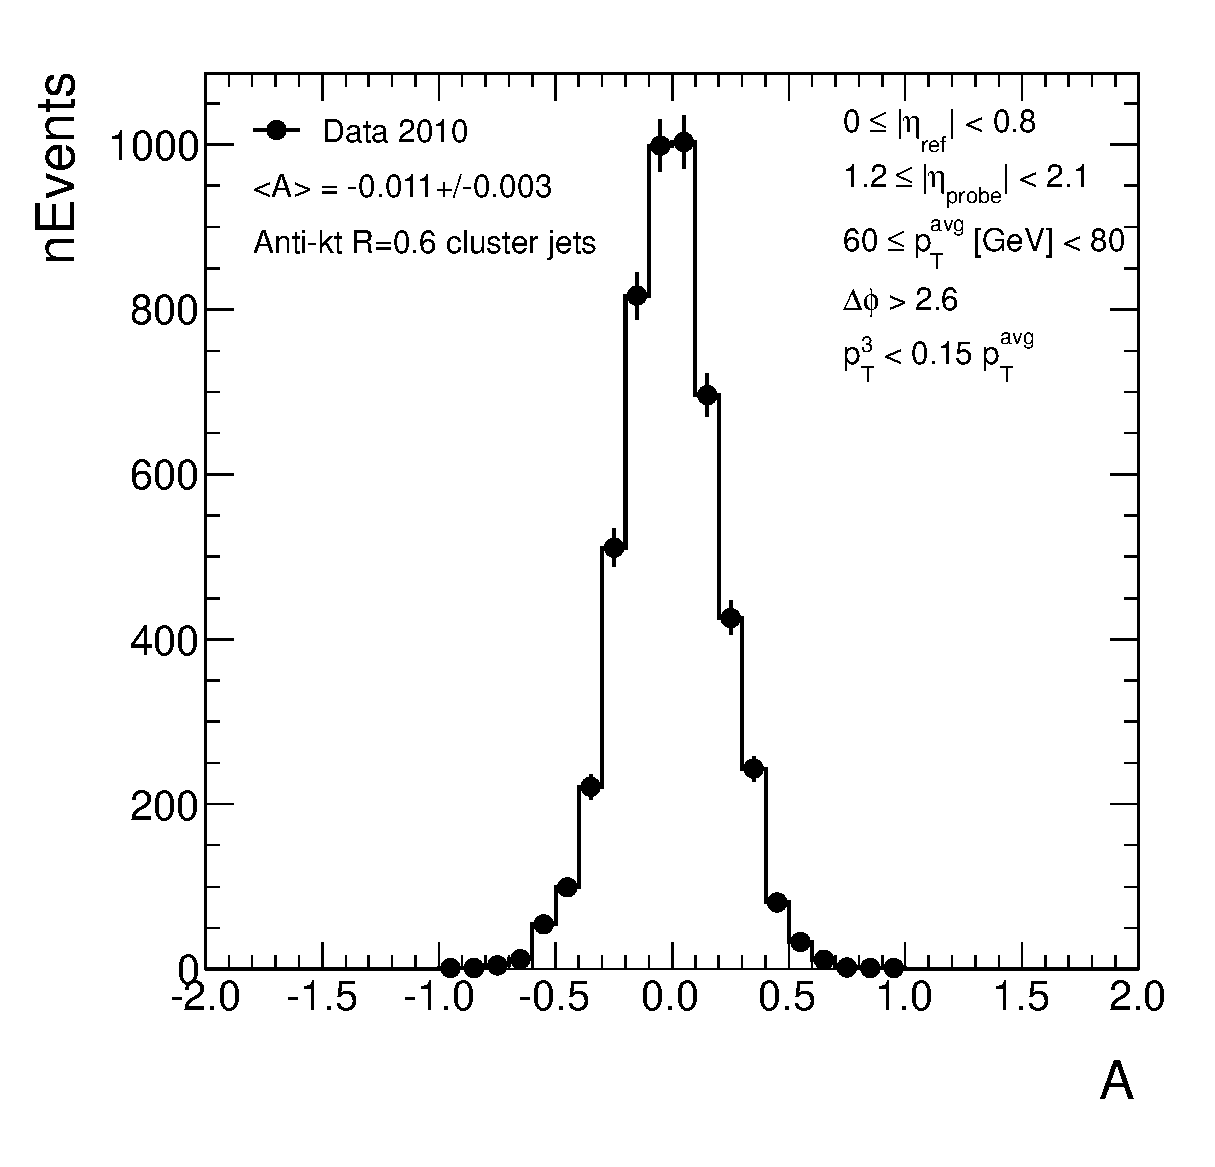
\includegraphics[width=\mediumfigwidth]{chapters/eta-intercalibration/Data.AntiKt6.refJetEta0_0.8.probeJetEta1.2_2.1.PTBinned.60_80.eps}
  \caption{A sample \Asymmetry distribution using \akt jets with $R=0.6$ and
           requiring that $\DeltaPhi(j_1,j_2) > 2.6$ and $60 \leq \pTavg < \unit{80}{\GeV}$
           with the reference jet falling into the region $\absEta < 0.8$ and the
           probe jet into the region $1.2 \leq \absEta < 2.1$.}
  \label{fig:etaint:sample_A_distribution}
\end{figure}

\subsection{Intercalibration using a Central Reference Region with a Soft-Radiation Correction}
As already discussed, a disadvantage with the method outlined above is that the
effects of soft radiation are hard to quantify and hence hard to correct for.
One solution to this is to apply a series of increasing cuts on the \pT of the
third hardest jet in the event and to extrapolate the information to the case in
which the third jet has zero \pT; in other words, the case in which there is no
soft radiation in the event. As can be seen from \FigureRef{fig:etaint:sample_extrapolation},
this can be done using a simple linear fit. The contents of each bin are, by definition,
highly correlated, since each bin is a superset of the previous one. Accordingly,
the best fit line was obtained by taking the covariance between the points into
account and minimising:

\begin{equation}
  \chi^2(\theta) = \sum_{i,j=1}^n \left(y_i - f(x_i, \theta)\right) V^{-1}_{ij} \left(y_j - f(x_j, \theta)\right)
\end{equation}

\noindent with respect to $\theta$. Here $f(x_i,\theta)$ is a simple linear function
in $x_i$, with $\theta$ representing the two free variables. The covariance matrix
$V$ is estimated using $V_{ij} = \frac{c_{ij}}{\sqrt{n_i n_j}}$, where $c_{ij}$ is the number
of events held in common between points $i$ and $j$ while $n_i$ and $n_j$ are the
total number of events contributing to each of these points.

\begin{figure}[htpb]
  \subfloat[\Asymmetry distribution for $\pT(j_3) / \pTavg < 0.19$]{
    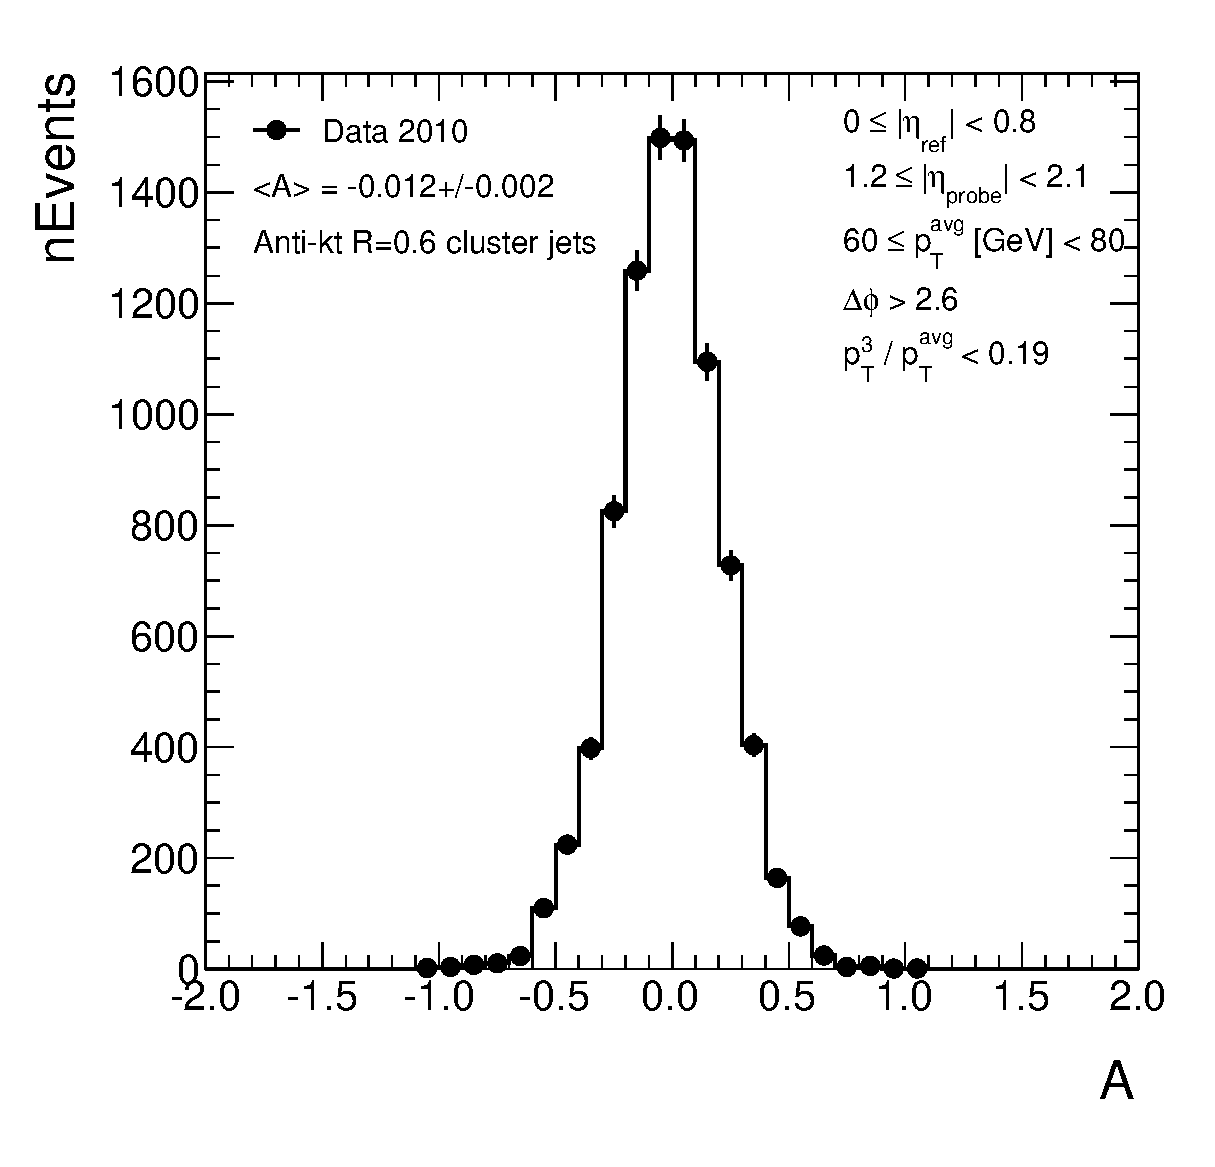
\includegraphics[width=\smallfigwidth]{chapters/eta-intercalibration/Data.AntiKt6.refJetEta0_0.8.probeJetEta1.2_2.1.PTBinned60_80.pT3_0.19.eps}
    \label{fig:etaint:sample_A_distribution_with_pT3_cut}}
  \quad
  \subfloat[Extrapolation to $\pT(j_3) = 0$]{
    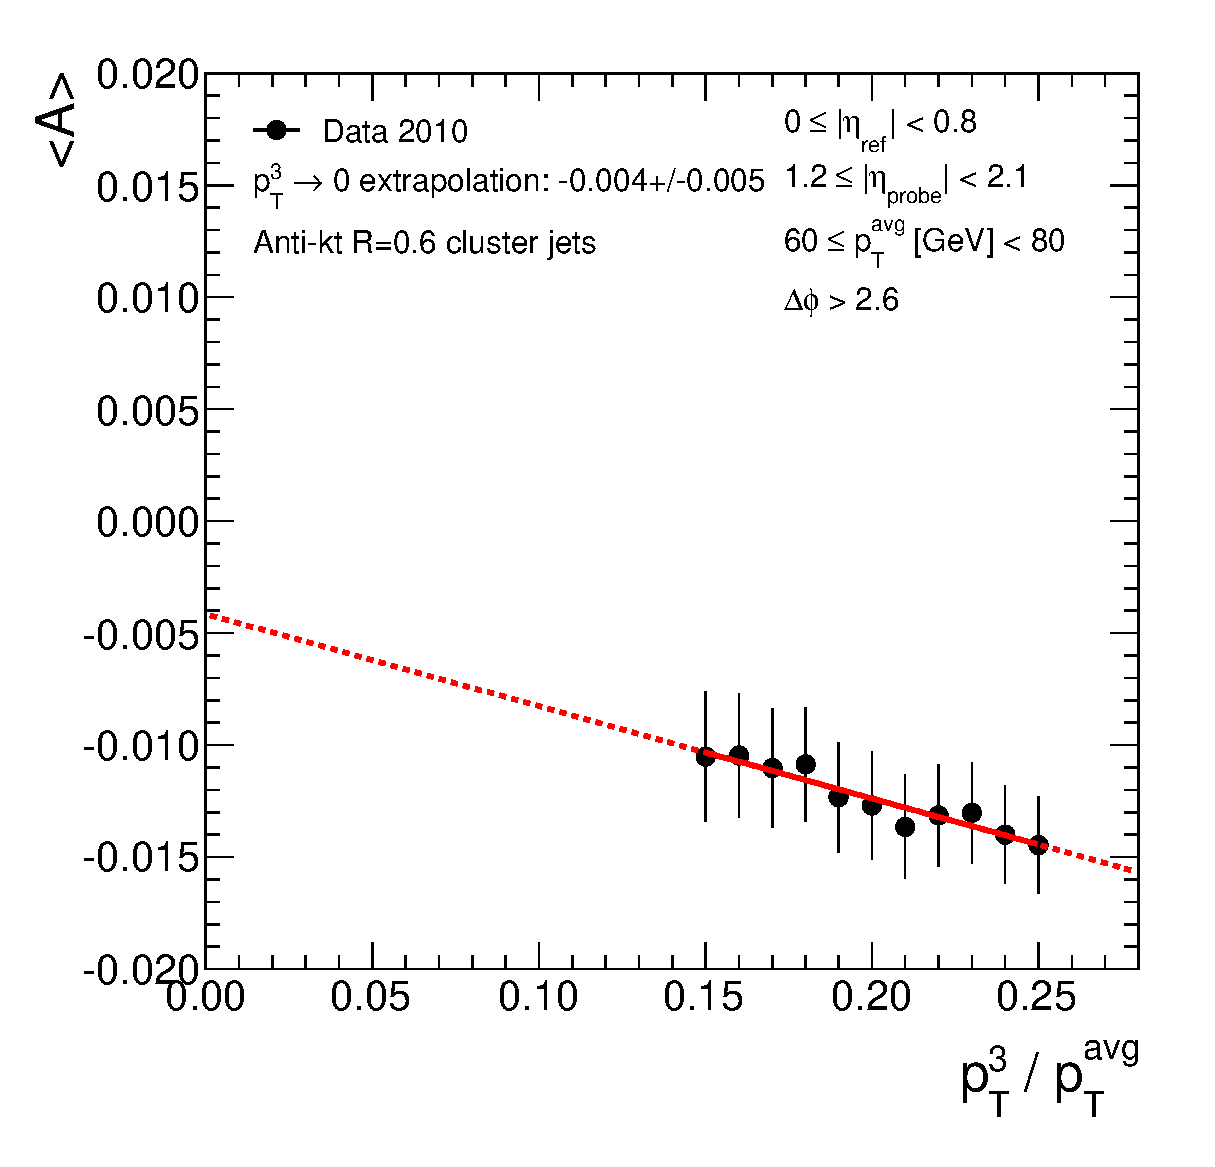
\includegraphics[width=\smallfigwidth]{chapters/eta-intercalibration/Data.AntiKt6.Extrapolation.refJetEta0_0.8.probeJetEta1.2_2.1.PTBinned.60_80.eps}
    \label{fig:etaint:sample_extrapolation}}
  \caption{A sample \Asymmetry distribution using \akt jets with $R=0.6$ and requiring
           that $\DeltaPhi(j_1,j_2) > 2.6$ and $60 \leq \pTavg < \unit{80}{\GeV}$,
           with the reference jet falling into the region $\absEta < 0.8$ and the
           probe jet into the region $1.2 \leq \absEta < 2.1$. \protect\subref{fig:etaint:sample_A_distribution_with_pT3_cut}
           is the \Asymmetry distribution for events which additionally satisfy
           $\pT(j_3) / \pTavg < 0.19$, while \protect\subref{fig:etaint:sample_extrapolation}
           shows the extrapolation from several different cuts on $\pT(j_3) / \pTavg$
           to the case in which $\pT(j_3) = 0$.}
  \label{fig:etaint:sample_thirdjet_curves}
\end{figure}

\section{Event Selection}
As discussed in \SectionRef{sec:analysis-tools:data_selection}, events are
required to belong to a good run and to have at least one good primary vertex.
For this analysis, the vertex requirement is tightened: only events with exactly
one good primary vertex are considered.

Events are required to possess at least two jets above the jet reconstruction
threshold of \unit{7}{\GeV}. The event is rejected if either of the two leading
jets are flagged as ``bad'' or ``ugly'' by the standard loose jet cleaning cuts,
discussed in \SectionRef{sec:analysis-tools:jet_cleaning}.

A trigger is assigned for each event, based on the run period and on \pTavg of
the \dijet pair. If this trigger is passed then the event is accepted. In later
periods, instead of a single trigger per event, two triggers are assigned, one
from the forward trigger system and one from the central trigger system. The
thresholds are chosen such that the trigger efficiency for each specific region
of \pTavg is greater than 99\% and is approximately flat as a function of the
pseudorapidity of the probe jet. To cover the low \pT region, $\pT < \unit{40}{\GeV}$,
as well as in early data taking when the trigger rates were low, triggers from
the minimum bias stream are used. These require at least one hit in the Minimum
Bias Trigger Scintillators (MBTS), which cover the region $2.08 \leq \absEta < 3.8$.
Forward triggers are not used before period E5, due to calibration problems.

\TableRef{tab:etaint:triggers} summarises the triggers used in the \etaint
measurement as a function of \pTavg and run period. As outlined in \SectionRef{sec:analysis-tools:jet_selection_evolution},
the lowest prescaled fully efficient jet trigger in each \pTavg bin changes over
time. All of these triggers are over 99\% efficient in the relevant regions.

\begin{table}
\begin{center}
  \begin{tabular}{ l l l @{\hspace{1.5cm}}l }
  \pTavg range $[\GeV]$ & Period A*   & Period B--D & Period E1--4 \\
  \midrule
  20--40                & L1\_MBTS\_1 & L1\_MBTS\_1 & L1\_MBTS\_1  \\
  40--50                & L1\_MBTS\_1 & L1\_J5      & L1\_J5       \\
  50--110               & L1\_J10     & L1\_J10     & L1\_J10      \\
  110--160              & L1\_J30     & L1\_J30     & L1\_J30      \\
  160+                  & L1\_J55     & L1\_J55     & L1\_J55      \\
  \midrule
  \pTavg range $[\GeV]$ & Period E5--F        & \multicolumn{2}{l}{Period G--H}                            \\
  \midrule
  20--40                & L1\_MBTS\_1         & \multicolumn{2}{l}{EF\_mbMbts\_1\_eff}                    \\
  40--50                & L1\_J5              & \multicolumn{2}{l}{EF\_mbMbts\_1\_eff}                    \\
  50--110               & L1\_J10 or L1\_FJ10 & \multicolumn{2}{l}{EF\_j30\_jetNoEF or EF\_fj30\_jetNoEF} \\
  110--160              & L1\_J30 or L1\_FJ30 & \multicolumn{2}{l}{EF\_j50\_jetNoEF or EF\_fj50\_jetNoEF} \\
  160+                  & L1\_J55 or L1\_FJ30 & \multicolumn{2}{l}{EF\_j75\_jetNoEF or EF\_fj75\_jetNoEF} \\
  \end{tabular}
  \caption{The trigger chains used for the \etaint analysis. The forward jet
           trigger could not be used in the first four periods (A--D) as it had
           not yet been commissioned, while additional problems made it
           unreliable for subperiods E1--4. L1\_MBTS\_1 was also used to trigger
           all jets before run 152777. The period after this timing change is
           denoted here as ``A*''.}
  \label{tab:etaint:triggers}
\end{center}
\end{table}

The \MC datasets which are compared to the data were generated using \Pythia,
\Herwigpp, \Alpgen and the \Perugia \Pythia tune, using the parameters described
in \SectionRef{sec:bg-theory:MC_generators}.

\section{\Dijet Balance Results}
In this section, the relative jet response obtained with the extrapolation
method is compared to the relative jet response obtained using the standard
method with a fixed cut on maximum $\pT(j_3)$. \FigureRef{fig:etaint:method_comparison_vs_eta}
shows the jet response relative to central jets, \relResponse, for two \pTavg-bins:
$30 \leq \pTavg < \unit{45}{\GeV}$ and $60 \leq \pTavg < \unit{80}{\GeV}$. These
results indicate that the response observed using the extrapolation method is
compatible with that obtained using the standard method. The results shown here
are representative of all the phase space regions considered in this analysis;
the extrapolation method is therefore used to give the final results for data
due to its more advanced treatment of residual soft effects; in the forward region,
where statistics in some \MC datasets are poor, this unfortunately results in large
errors.
%the standard method is retained for
%the \MC datasets as these suffer from poor statistics, particularly in the
%forward region.

\begin{figure}[htpb]
  \subfloat[$30 \leq \pTavg < \unit{45}{\GeV}$]{
    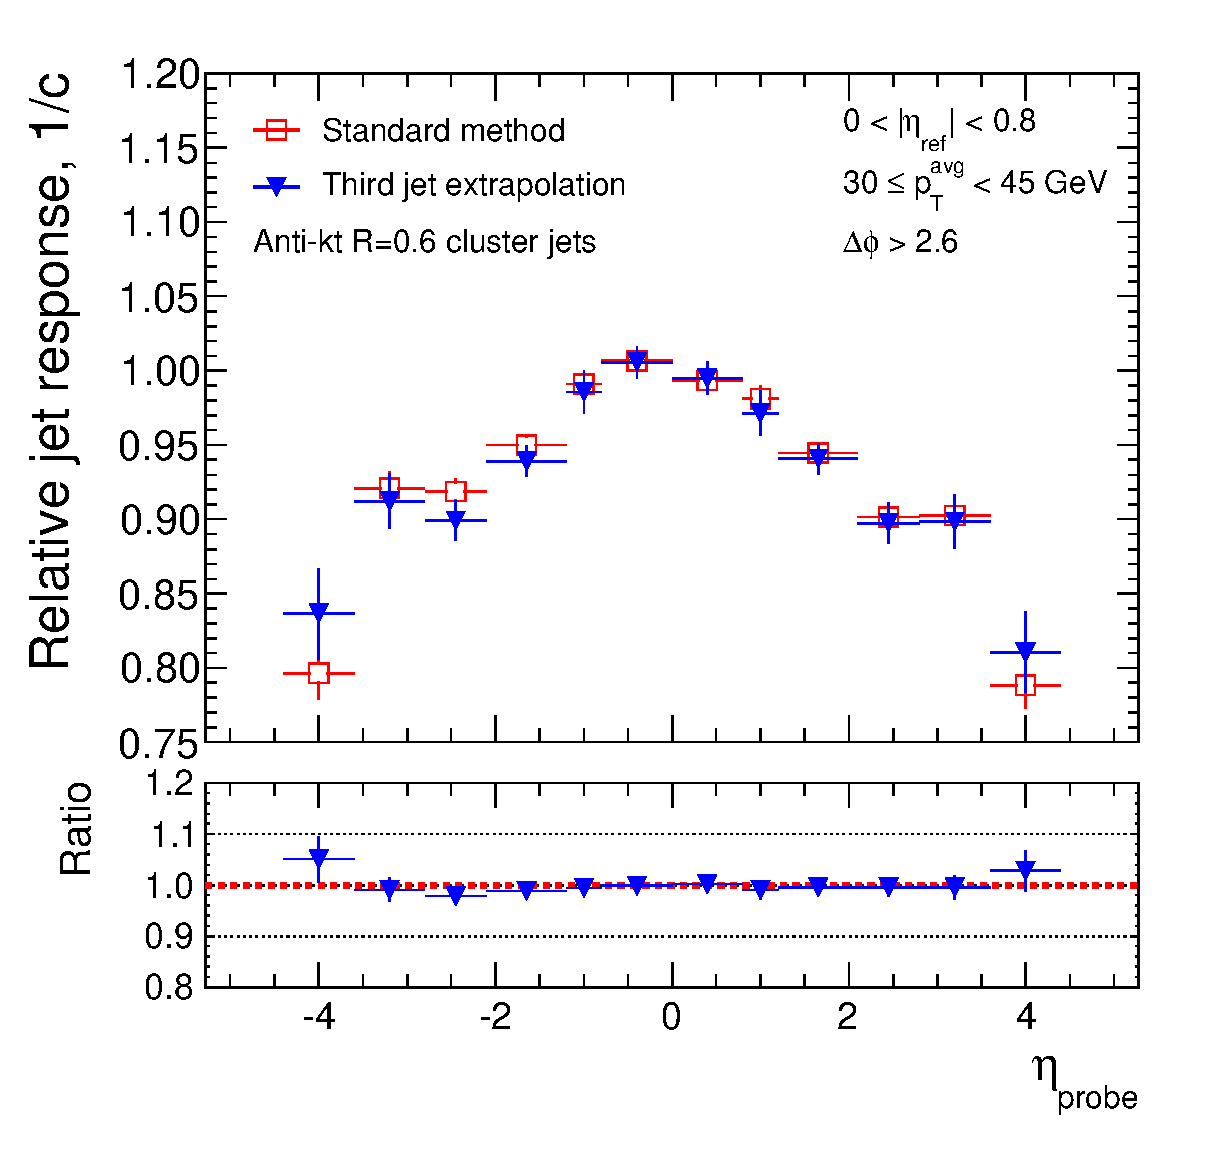
\includegraphics[width=\smallfigwidth]{chapters/eta-intercalibration/AntiKt6.refJetEta0_0.8.pTbar30_45.EtaBinned.MethodComparison.eps}
    \label{fig:etaint:method_comparison_vs_eta_pt30_45}}
  \quad
  \subfloat[$60 \leq \pTavg < \unit{80}{\GeV}$]{
    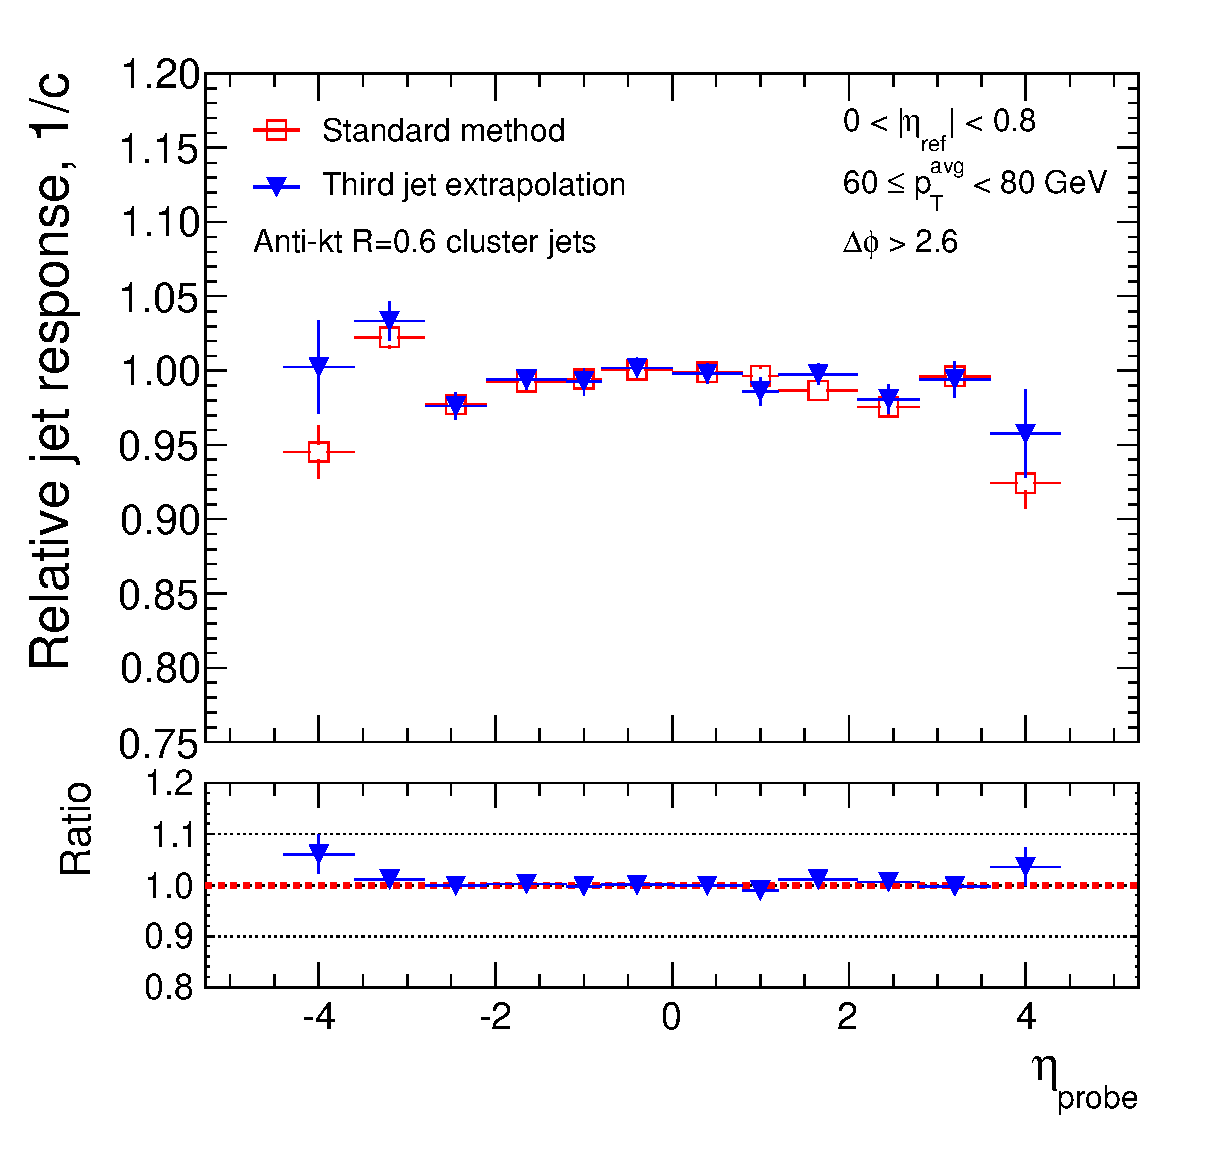
\includegraphics[width=\smallfigwidth]{chapters/eta-intercalibration/AntiKt6.refJetEta0_0.8.pTbar60_80.EtaBinned.MethodComparison.eps}
    \label{fig:etaint:method_comparison_vs_eta_pt60_80}}
  \caption{Relative jet response, 1/\relResponse, as a function of the
           pseudorapidity of the probe jet. Results are presented for two bins
           of \pTavg: \protect\subref{fig:etaint:method_comparison_vs_eta_pt30_45} $30 \leq \pTavg < \unit{45}{\GeV}$
           and \protect\subref{fig:etaint:method_comparison_vs_eta_pt60_80} $60 \leq
           \pTavg < \unit{80}{\GeV}$.}
  \label{fig:etaint:method_comparison_vs_eta}
\end{figure}

\FigureRef{fig:etaint:relative_jet_response_vs_eta} shows the relative response
obtained with the extrapolation method as a function of the jet pseudorapidity
for data and the \MC event generator simulations. Four different \pTavg regions
are shown: $20 \leq \pTavg < \unit{30}{\GeV}$, $30 \leq \pTavg < \unit{45}{\GeV}$,
$60 \leq \pTavg < \unit{80}{\GeV}$ and $80 \leq \pTavg < \unit{110}{\GeV}$. The
response in data is reasonably well reproduced by the \MC simulations for
$\pT > \unit{60}{\GeV}$, with the \MC and data typically agreeing at better than
the 2\% level in the central region ($\absEta < 2.8$) and better than 5\%
in the forward region ($\absEta > 2.8$). At lower values of \pTavg, the data
 do not agree so well with the \MC simulations and the \MC simulations
themselves show a large spread around the data. For $20 \leq \pT < \unit{30}{\GeV}$,
the \MC deviates from the data by about 10\% for $\absEta > 2.8$, with the
different \MC simulations predicting both higher and lower responses than that
observed in the data. The main differences, due to residual low \pT jet effects
(see \SectionRef{sec:etaint:central_reference}), occur between \Pythia/\Perugia
and \Alpgen/\Herwigpp. The reason is that the \Pythia and \Perugia predictions
are based upon a \pT-ordered parton shower, Lund String hadronisation and the
\Pythia underlying event model, whereas the \Herwigpp and \Alpgen predictions
are based on an angular-ordered parton shower, cluster hadronisation and the
\Jimmy underlying event model. These differences therefore reflect a 
difference in physics modelling among the event generators.

\begin{figure}[htpb]
  \subfloat[$20 \leq \pTavg < \unit{30}{\GeV}$]{
    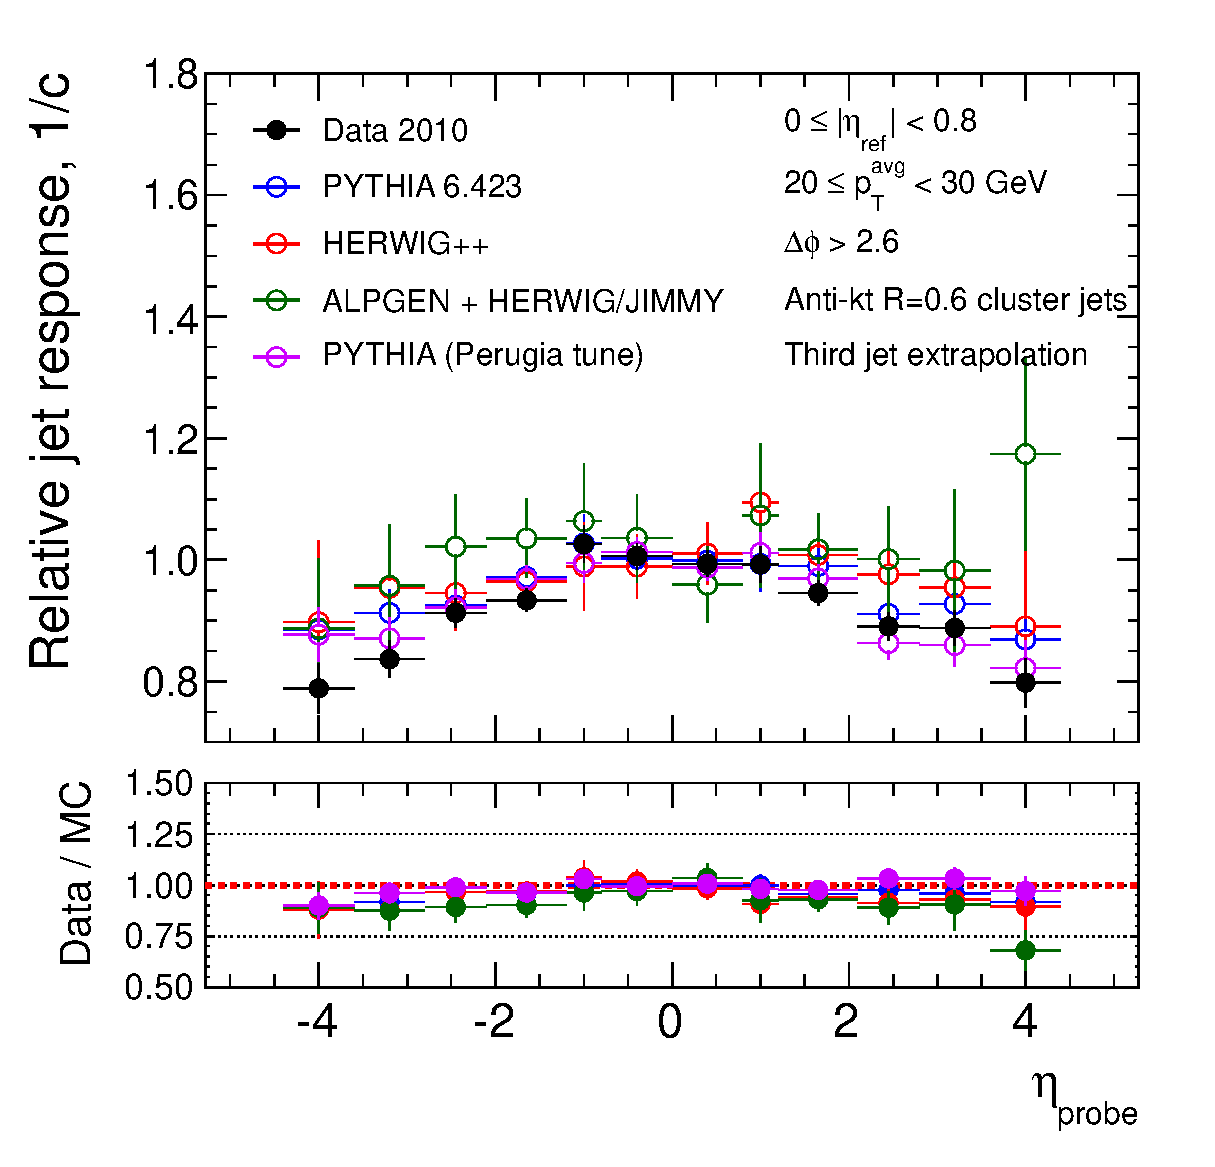
\includegraphics[width=\smallfigwidth]{chapters/eta-intercalibration/AntiKt6.refJetEta0_0.8.pTbar20_30.EtaBinned.ThirdJetExtrapolation.eps}
    \label{fig:etaint:relative_jet_response_vs_eta_pt20_30}}
  \quad
  \subfloat[$30 \leq \pTavg < \unit{45}{\GeV}$]{
    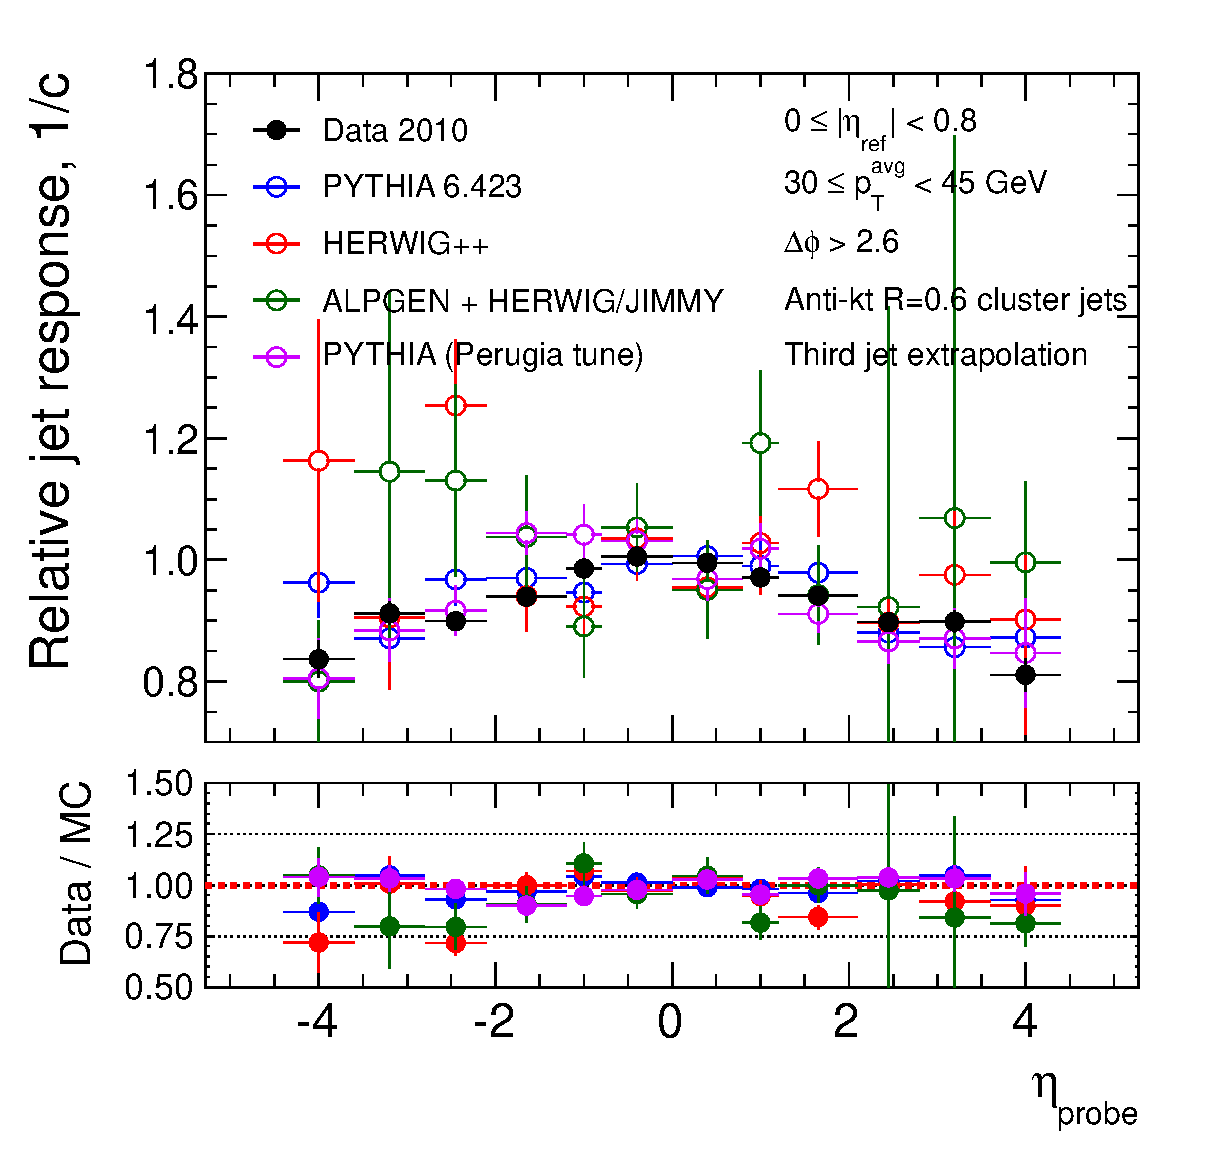
\includegraphics[width=\smallfigwidth]{chapters/eta-intercalibration/AntiKt6.refJetEta0_0.8.pTbar30_45.EtaBinned.ThirdJetExtrapolation.eps}
    \label{fig:etaint:relative_jet_response_vs_eta_pt30_45}}
  \\
  \subfloat[$60 \leq \pTavg < \unit{80}{\GeV}$]{
    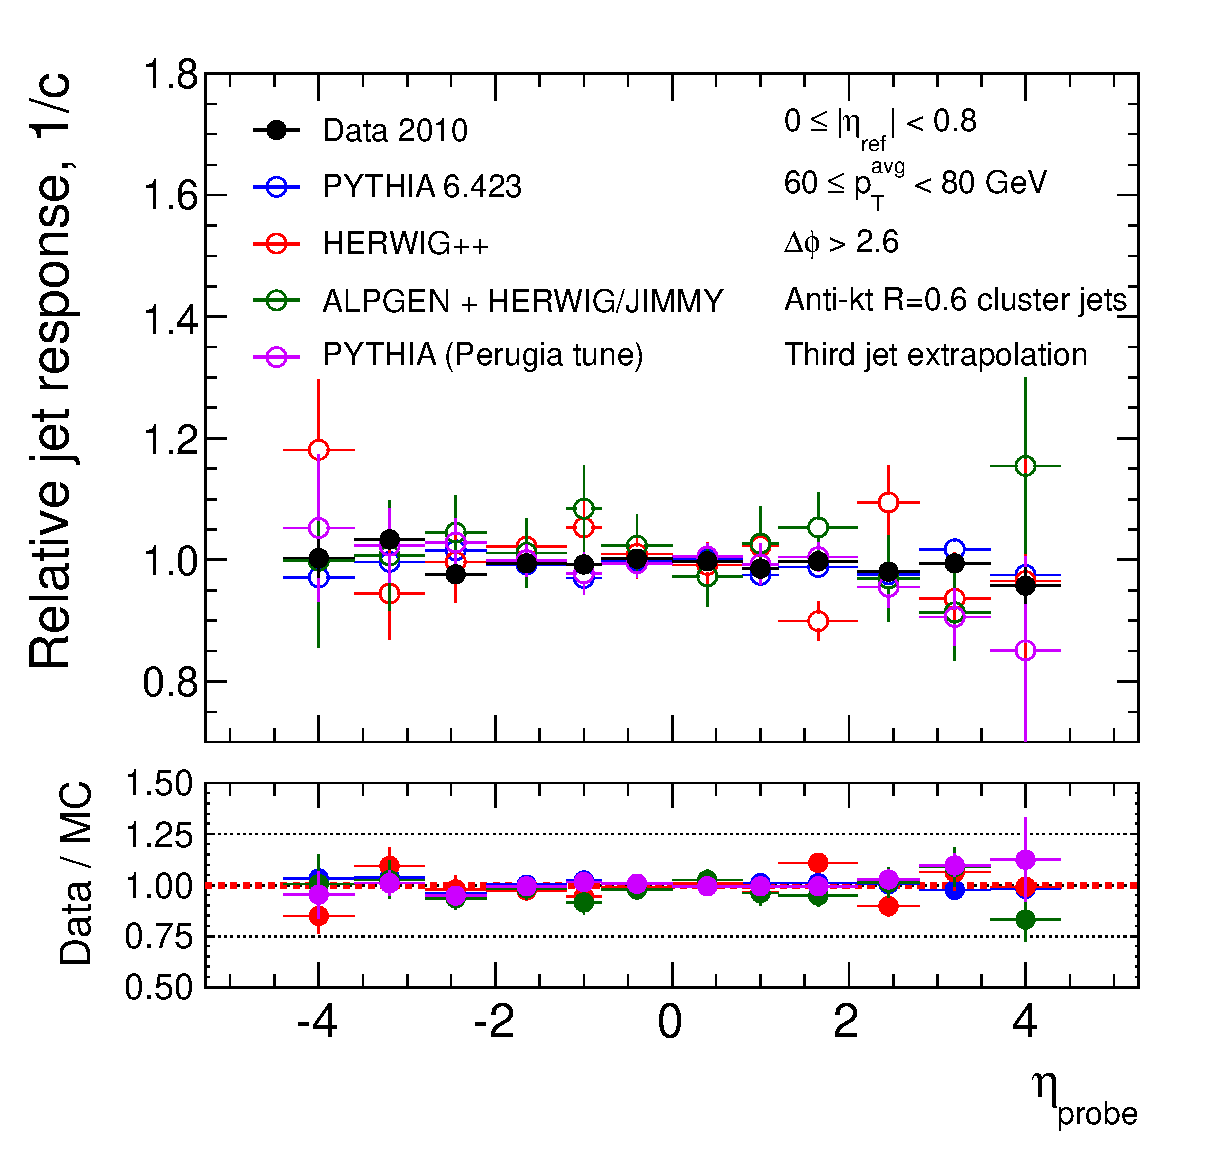
\includegraphics[width=\smallfigwidth]{chapters/eta-intercalibration/AntiKt6.refJetEta0_0.8.pTbar60_80.EtaBinned.ThirdJetExtrapolation.eps}
    \label{fig:etaint:relative_jet_response_vs_eta_pt60_80}}
  \quad
  \subfloat[$80 \leq \pTavg < \unit{110}{\GeV}$]{
    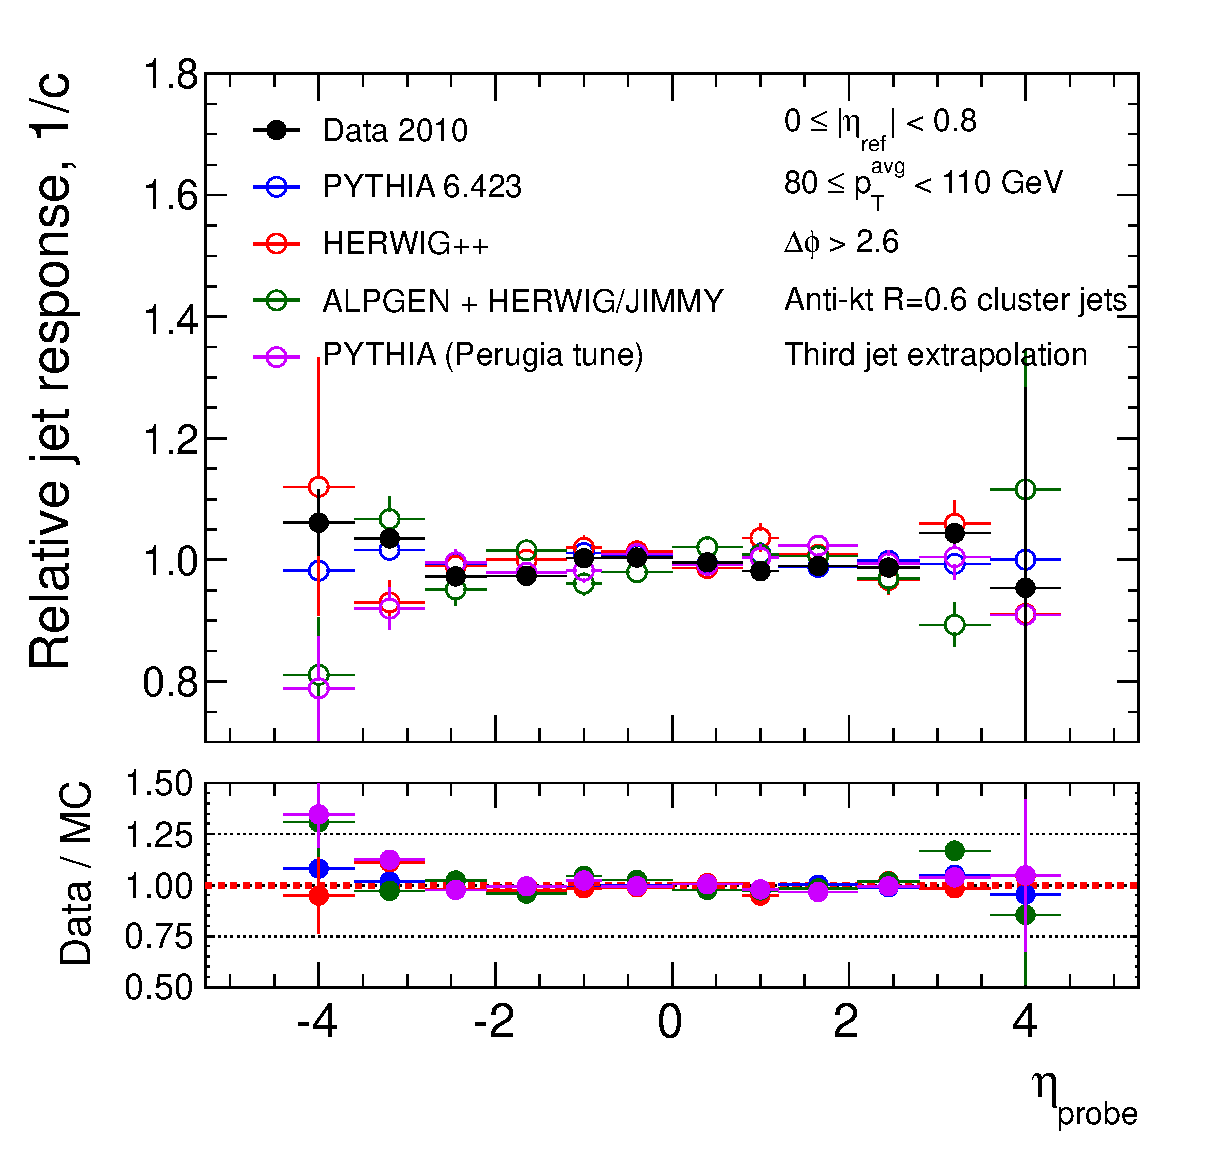
\includegraphics[width=\smallfigwidth]{chapters/eta-intercalibration/AntiKt6.refJetEta0_0.8.pTbar80_110.EtaBinned.ThirdJetExtrapolation.eps}
    \label{fig:etaint:relative_jet_response_vs_eta_pt80_110}}
  \caption{Relative jet response, 1/\relResponse, as a function of the \pseudorap
           of the probe jet. Results are presented for four bins of \pTavg:
           \protect\subref{fig:etaint:relative_jet_response_vs_eta_pt20_30} $20 \leq \pTavg < \unit{30}{\GeV}$,
           \protect\subref{fig:etaint:relative_jet_response_vs_eta_pt30_45} $30 \leq \pTavg < \unit{45}{\GeV}$,
           \protect\subref{fig:etaint:relative_jet_response_vs_eta_pt60_80} $60 \leq \pTavg < \unit{80}{\GeV}$
           and \protect\subref{fig:etaint:relative_jet_response_vs_eta_pt80_110} $80 \leq \pTavg < \unit{110}{\GeV}$.}
  \label{fig:etaint:relative_jet_response_vs_eta}
\end{figure}

\FigureRef{fig:etaint:relative_jet_response_vs_pt} shows the relative response as
a function of \pTavg. The distributions are shown for jets in the region $1.2 \leq \absEta < 2.1$
and also for those in the region $3.6 \leq \absEta < 4.4$. Again, the response
is reasonably well described by the \MC for all calorimeter regions at high
\pTavg and for the more central region at low \pTavg.

\begin{figure}[htpb]
  \subfloat[$1.2 \leq \absEta < 2.1$]{
    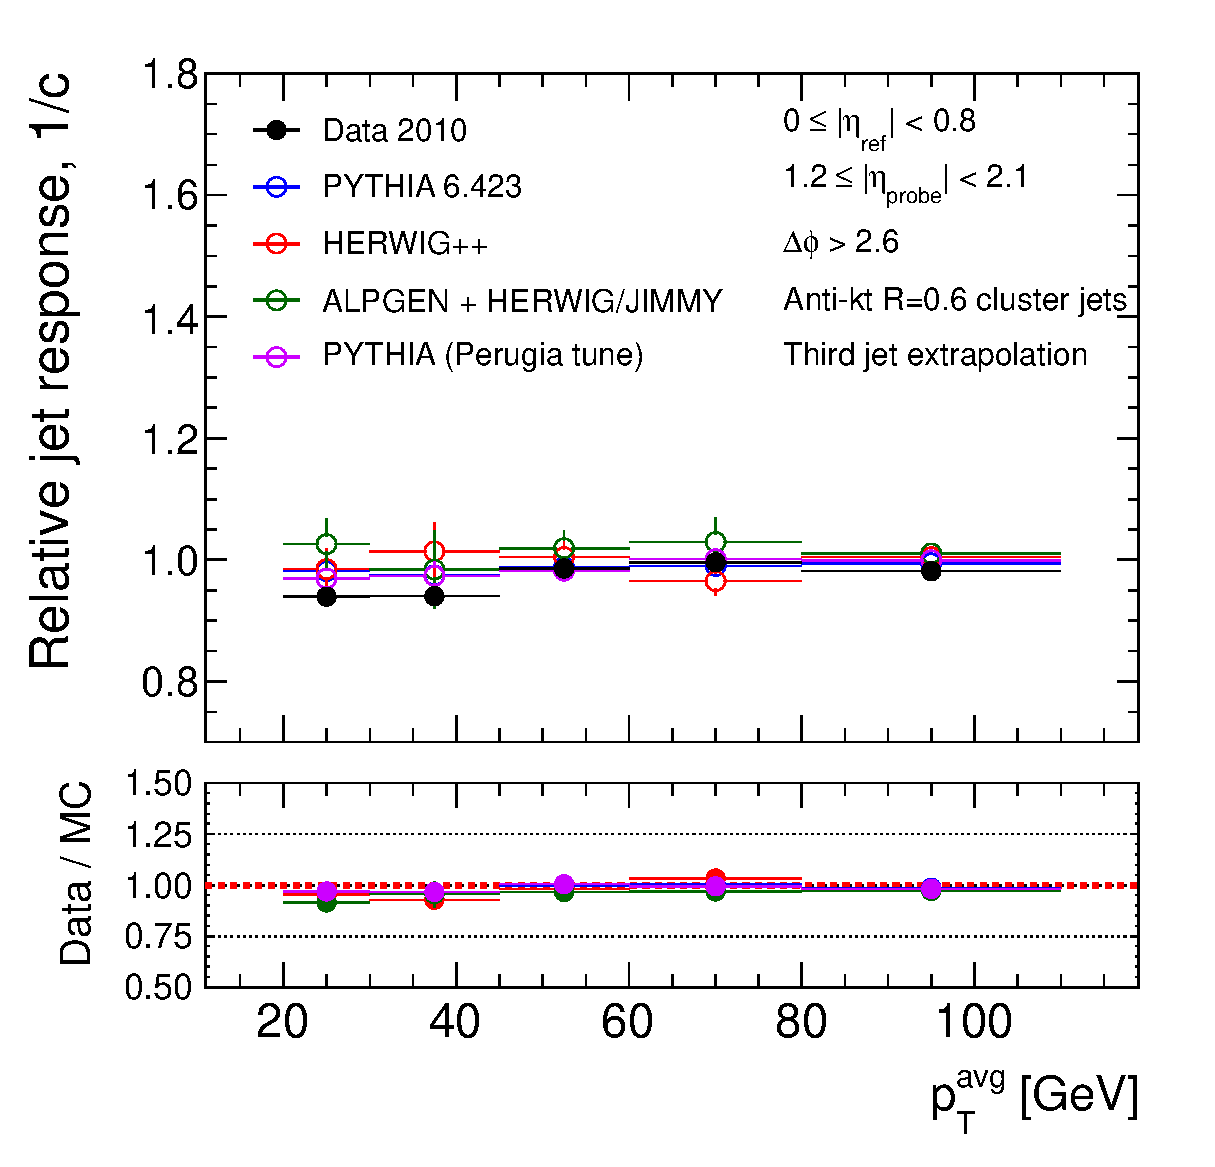
\includegraphics[width=\smallfigwidth]{chapters/eta-intercalibration/AntiKt6.refJetEta0_0.8.probeJetEta1.2_2.1.PTBinned.ThirdJetExtrapolation.eps}
    \label{fig:etaint:relative_jet_response_vs_pt_eta1.2_2.1}}
  \quad
  \subfloat[$3.6 \leq \absEta < 4.4$]{
    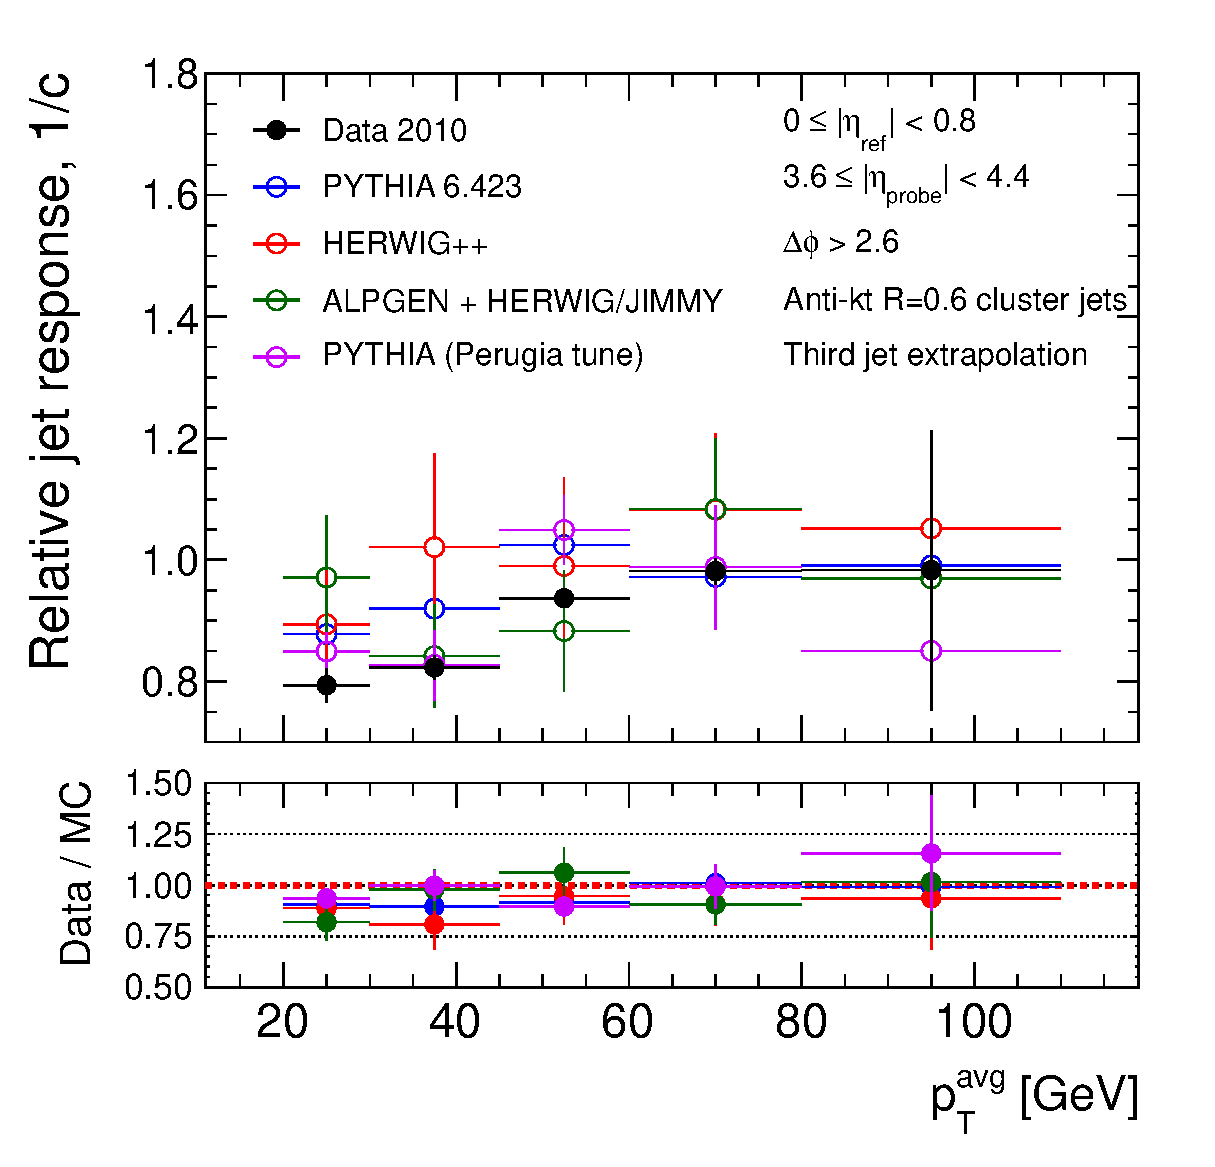
\includegraphics[width=\smallfigwidth]{chapters/eta-intercalibration/AntiKt6.refJetEta0_0.8.probeJetEta3.6_4.4.PTBinned.ThirdJetExtrapolation.eps}
    \label{fig:etaint:relative_jet_response_vs_pt_eta3.6_4.4}}
  \caption{Relative jet response, 1/\relResponse, as a function of the \pseudorap of the probe jet.
           For low \pTavg and early data periods, the data is collected using the minimum bias trigger stream. For
           higher \pTavg, the data is collected using the calorimeter trigger stream.
           Results are presented for two bins of \absEta: \protect\subref{fig:etaint:relative_jet_response_vs_pt_eta1.2_2.1}
           $1.2 \leq \absEta < 2.1$ and \protect\subref{fig:etaint:relative_jet_response_vs_pt_eta3.6_4.4}
           $3.6 \leq \absEta < 4.4$.}
  \label{fig:etaint:relative_jet_response_vs_pt}
\end{figure}


\section{Uncertainty due to Intercalibration}
In the previous section it was shown that the \MC predictions for the relative
jet response diverge at low values of \pTavg, with the data itself lying between
the different predictions for central values of \pseudorap. The uncertainty on
the relative jet response must reflect this disagreement because there is no \textit{a priori} reason to
believe one theoretical prediction over another. The uncertainty on the relative
response is taken to be the RMS deviation of the \MC predictions from the data.
At high \pTavg, where the spread of the \MC predictions is small, the
uncertainty mainly reflects the true difference between the response in data and
simulation. At low \pTavg and large \absEta, the uncertainty mainly reflects the
physics modelling uncertainty, although the detector-based differences between
data and simulation are also accounted for. The RMS spread of \MC predictions
around the data measurement is less sensitive to statistical fluctuations in
comparison to other possible measures of the deviation, such as the maximal
difference between the predictions or between data and \MC. The latter
quantities tend to give unstable results since all of the \MC samples used
in the analysis, aside from \Pythia, are generated with low statistics (for details see
\SectionRef{sec:bg-theory:MC_generators}); \MC generators with fewer than ten
entries in a particular bin of $|\etaProbe|$ and \pTavg are excluded from that bin
of the RMS calculation for this reason.

\begin{figure}[htpb]
  \subfloat[Uncertainty in the jet response as a function of \dijet \pTavg in five regions of the calorimeter.]{
    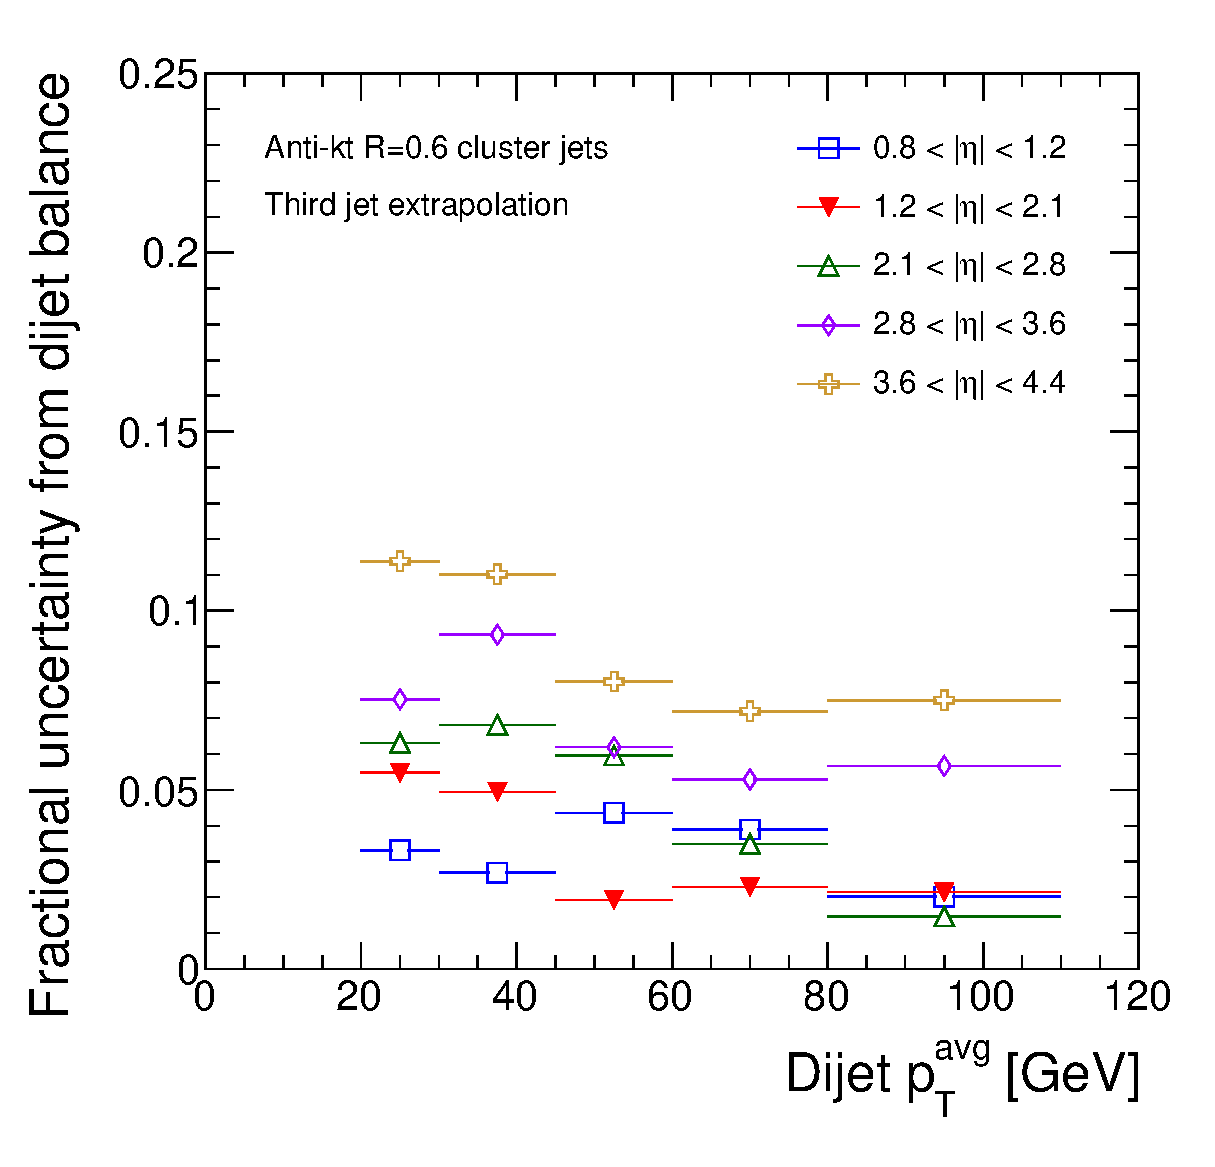
\includegraphics[width=\smallfigwidth]{chapters/eta-intercalibration/AntiKt6.JetResponseUncertainty.PTBinned.eps}
    \label{fig:etaint:relative_jet_response_uncertainty_vs_pt}}
  \quad
  \subfloat[Uncertainty in the jet response as a function of jet $\absEta$ for five values of \dijet \pTavg.]{
    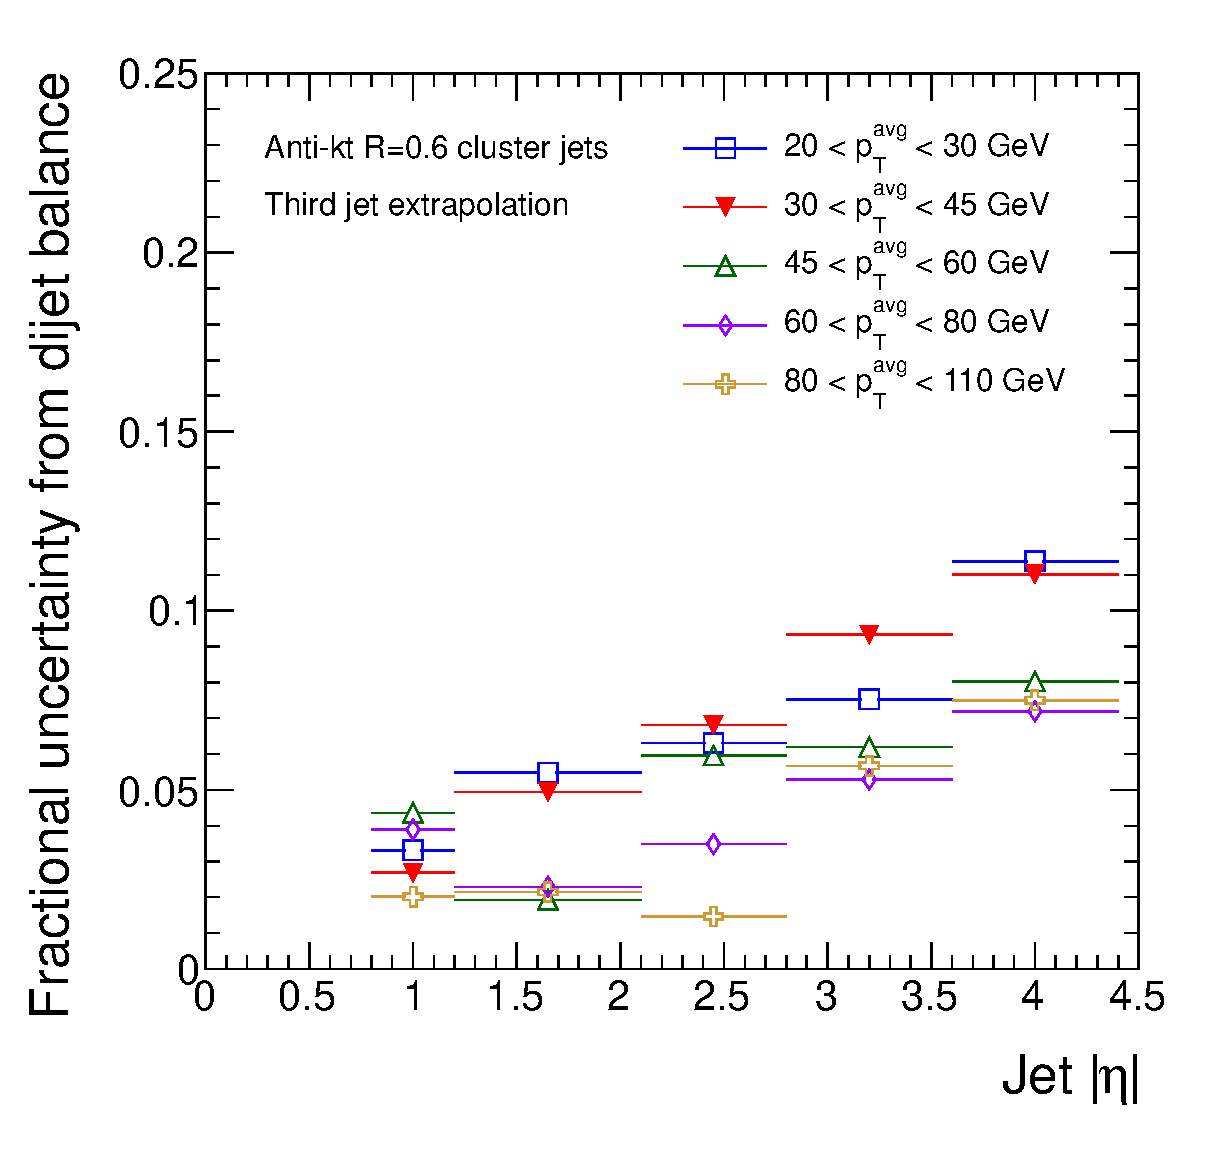
\includegraphics[width=\smallfigwidth]{chapters/eta-intercalibration/AntiKt6.JetResponseUncertainty.EtaBinned.eps}
    \label{fig:etaint:relative_jet_response_uncertainty_vs_eta}}
  \caption{Fractional uncertainty in the relative jet response, 1/\relResponse, arising from \dijet
           balance as a function of \protect\subref{fig:etaint:relative_jet_response_uncertainty_vs_pt} the \pTavg
           and \protect\subref{fig:etaint:relative_jet_response_uncertainty_vs_eta} the
           \pseudorap of the \dijet system.}
  \label{fig:etaint:relative_jet_response_uncertainty}
\end{figure}

\FigureRef{fig:etaint:relative_jet_response_uncertainty} shows the uncertainty in the jet response,
relative to jets in the region $\absEta < 0.8$, as a function of the \dijet \pTavg and $\absEta$.

\section{Summary}
These results indicate that the relative response to jets with $\absEta \leq 0.8$
is well understood both for high \pT jets across the full calorimeter range and
for central jets across the \pT range considered. Deviations between
data and \MC are at their smallest for high \pT central jets, at about 3\%, and
at their worst for low \pT forward jets, at about 12\%. Additionally, different
\MC generators show a large spread of predictions in the low \pT region,
reflecting a real physics modelling uncertainty. This work was published as an
\ATLAS conference note~\cite{ATLAS-CONF-2011-014} and also formed one of
the inputs for the evaluation of the jet energy scale 
uncertainty~\cite{ATLAS-CONF-2010-056} (see \SectionRef{sec:analysis-tools:jes_uncertainty} for details)
which was submitted to European Physical Journal C~\cite{CERN-PH-EP-2011-191}. The
results shown here are in agreement with these published results, which use a slightly
different method of determining the response factors, $1/c$, providing increased
statistical precision.

  \chapter{Inclusive Jet \Xs{s}}
\label{chap:forward-inclusive}

\chapterquote{It's not exclusive, but inclusive, which is the whole spirit of
jazz.}{Herbie Hancock}

\section{Introduction}
As discussed in \SectionRef{sec:bg-theory:jets_in_hadron_colliders}, jet production
is the dominant high \pT process at the \LHC. Jet \xs{s} are important
observables in high-energy particle physics and are one of the first measurements
that can be performed in a hadron collider experiment. These \xs{s} are
an important tool for understanding the strong interaction, in particular through
providing precise measurements of \alphaS. In addition to testing \QCD in a
new kinematic regime, the data also provide sensitivity to different parton distribution
functions (PDFs) in a region where they are currently poorly constrained.

This analysis presents inclusive double-differential jet \xs{s}; studied
as a function of jet \pT and \rap. The measurement covers $\unit{20}{\GeV} \leq \pT < \unit{1.5}{\TeV}$
in the rapidity range $\absRap < 4.4$. The results are compared to theoretical predictions
from next-to-leading order \QCD corrected for non-perturbative effects, as well as
to next-to-leading order \MC simulations. The rapidity slices used in the measurement
have boundaries which follow the calorimeter geometry.

\section{\Xs Definition}
\label{sec:forward-inclusive:cross_section_definition}
Clearly, jet \xs{s} can only be defined for a specific jet algorithm;
here \xs{s} have been calculated for the \ATLAS standard: \akt jets with
$R=0.4$ and $R =0.6$ (see \SectionRef{bg-theory:recombination_algorithms} and
\SectionRef{sec:analysis-tools:jet_reconstruction}). The jet \xs measurements
are corrected for all experimental effects (see \SectionRef{sec:analysis-tools:unfolding}),
and so refer to the ideal particle level final state of a proton-proton
collision~\cite{Buttar:2008:toolsandjets}. In the \MC, particle level jets are
identified using the same jet algorithms applied to data, using stable particles,
all those with a proper lifetime longer than \unit{10}{\pico\second}, as their
input. This definition includes muons and neutrinos from decaying hadrons which
cannot be included in calorimeter jets reconstructed in data.

\section{Event Selection}
Following the outline in \SectionRef{sec:analysis-tools:data_selection}, events
are required to belong to a good run and to have at least one good primary
vertex. All jets in the event which satisfy $\pT \geq \unit{20}{\GeV}$ and
$\absRap < 4.4$ are retained unless they are flagged as ``bad'' or ``ugly'' by
the standard medium jet cleaning cuts (see \SectionRef{sec:analysis-tools:jet_cleaning}).
Each jet is then assigned a specific, fully-efficient trigger which depends on
its transverse momentum and rapidity, as well as the run period that the event
belongs to. For the jet to contribute towards the inclusive \xs, this trigger must be passed. All jets which pass their trigger are retained,
with a weight reflecting the amount of luminosity seen by the trigger, which, due
to prescaling, is usually less than then the total luminosity recorded by \ATLAS.

\section{Trigger Strategy}
\label{sec:forward-inclusive:trigger}
This measurement uses three different trigger systems (see \SectionRef{sec:detector:trigger}):
the Minimum Bias Trigger Scintillators (MBTS) are used to select events
containing jets with $20 \leq \pT < \unit{60}{\GeV}$, the central jet triggers are
used for the remainder of the phase space region $\absRap<3.6$ while the forward
jet triggers are used for jets with $3.2 \leq \absRap < 4.9$. In the region $3.2 \leq \absRap < 3.6$
a combination of central and forward jet triggers is used. The L1\_MBTS\_1
trigger has been demonstrated to have a negligible inefficiency in selecting
the low \pT events for which it is used here.

For this measurement, the rapidity interval $\absRap < 4.4$ was divided into seven
bins: the central bins with $\absRap < 2.8$, the HEC-FCAL transition bin with $2.8 \leq \absRap < 3.6$
and the forward bin with $\absRap \geq 3.6$. As discussed in \SectionRef{sec:analysis-tools:jet_selection_evolution},
increasing instantaneous luminosity throughout 2010 means that the lowest prescaled
fully efficient trigger in each \pT bin changes over time.

\TableRangeRef{tab:forward-inclusive:TriggersCentral}{tab:forward-inclusive:TriggersForward}
summarise the triggers that are used in each \pT bin of the \xs measurement
as a function of the data taking period. For the central bins, these are central jet
triggers and for the forward bin, forward jet triggers. In both cases, certain
bins are augmented by data taken using the L1\_MBTS\_1 trigger. It is confirmed
that all of these triggers are over 99\% efficient in these regions.

\begin{table}
\begin{center}
  \begin{tabular}{ l l l l l }
             & \multicolumn{2}{c}{Period A*--F}         & \multicolumn{2}{c}{Period G--I}               \\
                    \cmidrule(lr){2-3}                         \cmidrule(lr){4-5}
  \pT range  & Central       & Central crack            & Central           & Central crack             \\
  {[}\GeV{]} & $\absRap<2.8$ & $1.2 \leq \absRap < 2.1$ & $\absRap<2.8$     &  $1.2 \leq \absRap < 2.1$ \\
             & except crack  &                          & except crack      &                           \\
  \midrule
  60--80     & L1\_J5        &  L1\_J5                  & EF\_j20\_jetNoEF  & EF\_j20\_jetNoEF          \\
  80--110    & L1\_J15       &  L1\_J5                  & EF\_j35\_jetNoEF  & EF\_j20\_jetNoEF          \\
  110--160   & L1\_J30       &  L1\_J15                 & EF\_j50\_jetNoEF  & EF\_j35\_jetNoEF          \\
  160--210   & L1\_J55       &  L1\_J30                 & EF\_j75\_jetNoEF  & EF\_j50\_jetNoEF          \\
  210--260   & L1\_J75       &  L1\_J55                 & EF\_j95\_jetNoEF  & EF\_j75\_jetNoEF          \\
  260--310   & L1\_J95       &  L1\_J75                 & EF\_L1J95\_NoAlg  & EF\_j95\_jetNoEF          \\
  310--400   & L1\_J95       &  L1\_J95                 & EF\_L1J115\_NoAlg & EF\_L1J95\_NoAlg          \\
  400+       & L1\_J95       &  L1\_J95                 & EF\_L1J115\_NoAlg & EF\_L1J115\_NoAlg         \\
  \end{tabular}
  \caption{The trigger chains used for the inclusive jet analysis in the region
           $\absRap<2.8$. The L1\_MBTS\_1 trigger is used for the $20 \leq \pT < \unit{60}{\GeV}$
           over the range $\absRap<2.8$. Due to mistimings in the Level-1 central
           jet trigger hardware, L1\_MBTS\_1 was also used to trigger all jets before
           run 152777. The period after this timing change is here denoted as ``A*''.}
  \label{tab:forward-inclusive:TriggersCentral}
\end{center}
\end{table}

\begin{table}
\begin{center}
  \begin{tabular}{ l l l l }
  \pT range $[\GeV]$ & Period A--C & Period E5--F & Period G--I       \\
  \midrule
  20--30             & L1\_MBTS\_1 & n/a          & n/a               \\
  30--45             & n/a         & L1\_FJ10     & n/a               \\
  45--60             & n/a         & L1\_FJ10     & n/a               \\
  60--80             & n/a         & L1\_FJ10     & EF\_fj30\_jetNoEF \\
  80--110            & n/a         & L1\_FJ30     & EF\_fj30\_jetNoEF \\
  110--160           & n/a         & L1\_FJ55     & EF\_fj50\_jetNoEF \\
  160--210           & n/a         & L1\_FJ55     & EF\_fj75\_jetNoEF \\
  210--260           & n/a         & L1\_FJ55     & EF\_fj75\_jetNoEF \\
  260+               & n/a         & L1\_FJ55     & EF\_fj75\_jetNoEF \\
  \end{tabular}
  \caption{The trigger chains used for the inclusive jet analysis in the forward
           region, $3.6 \leq \absRap < 4.4$. The first four periods (A--D) could not
           be used, as the forward jet trigger had not yet been commissioned, while
           additional problems made it unreliable for subperiods E1--4. L1\_MBTS\_1
           was found to be fully efficient for forward jets and hence was used in
           early periods to trigger low \pT forward jets.}
  \label{tab:forward-inclusive:TriggersForward}
\end{center}
\end{table}

\subsection{Trigger Strategy in the Transition Region}
\label{sec:forward-inclusive:transition_triggers}
A jet is accepted as having passed its particular inclusive trigger requirement if
at least one jet in the event has passed that trigger. Due to the reduced
\pseudorap-granularity available in the trigger system, it is therefore possible
for jets in the forward region to belong to an event in which only central trigger
chains have fired, or \emph{vice versa}. Events of this type will predominantly fall into
the HEC-FCAL transition region, $2.8 \leq \absRap < 3.6$. Additionally, it is possible
that jets in this region might trigger both the central and forward trigger systems.
It can be seen in \FigureRef{fig:forward-inclusive:eta_efficiency_akt} that, when taking
central and forward triggers with the same \ETEM threshold, the logical OR of the
two triggers is fully efficient across this transition region although neither trigger
is on its own.

\begin{figure}[htpb]
  \subfloat[\Akt $R=0.4$ jets, 2010 data]{
    \includegraphics[width=\smallfigwidth]{chapters/forward-inclusive/TriggerEfficiency.akt4.data.eps} %eta_efficiency_akt4.eps}
    \label{fig:forward-inclusive:eta_efficiency_data_akt4}}
  \quad
  \subfloat[\Akt $R=0.6$ jets, 2010 data]{
    \includegraphics[width=\smallfigwidth]{chapters/forward-inclusive/TriggerEfficiency.akt6.data.eps} %eta_efficiency_akt6.eps}
    \label{fig:forward-inclusive:eta_efficiency_data_akt6}}
  \\
  \subfloat[\Akt $R=0.4$ jets, \Pythia]{
    \includegraphics[width=\smallfigwidth]{chapters/forward-inclusive/TriggerEfficiency.akt4.pythia.eps} %eta_efficiency_akt4.eps}
    \label{fig:forward-inclusive:eta_efficiency_pythia_akt4}}
  \quad
  \subfloat[\Akt $R=0.6$ jets, \Pythia]{
    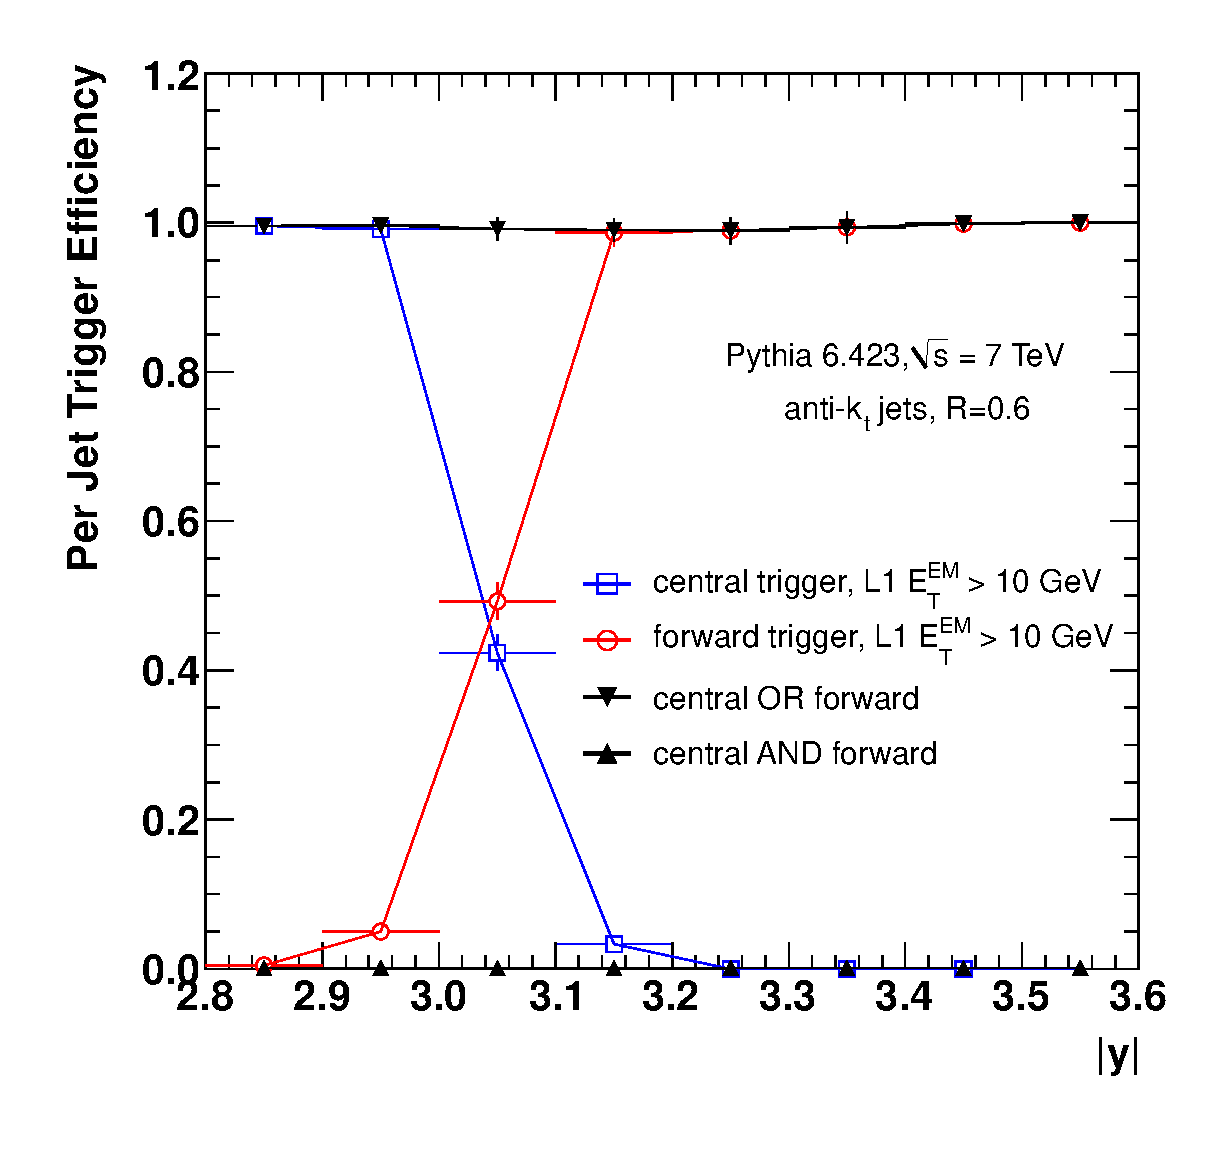
\includegraphics[width=\smallfigwidth]{chapters/forward-inclusive/TriggerEfficiency.akt6.pythia.eps} %eta_efficiency_akt6.eps}
    \label{fig:forward-inclusive:eta_efficiency_pythia_akt6}}
  \caption{Efficiency of the central and forward trigger signatures J10 and FJ10,
           their AND and their OR, as a function of rapidity, \rap, of the offline jet.
           Trigger efficiency is shown in data (top) and in \MC (bottom) while
           \akt $R=0.4$ jets (left) and \akt $R=0.6$ jets (right) are also considered
           separately.}
  \label{fig:forward-inclusive:eta_efficiency_akt}
\end{figure}

Sample turn-on curves for the central OR forward combination can be
seen in \FigureRef{fig:forward-inclusive:transition_bin_trigger_efficiencies}, demonstrating
that this combination is fully efficient at sufficiently high jet \pT. \TableRef{tab:forward-inclusive:TriggersTransition}
summarises the triggers that are used in each \pT bin of the \xs measurement
as a function of the data taking period.

\begin{figure}[htpb]
  \subfloat[L1 efficiency, \akt $R=0.4$ jets]{
    \includegraphics[width=\smallfigwidth]{chapters/forward-inclusive/transition_bin_triggers_L1_akt4.eps}
    \label{fig:forward-inclusive:transition_bin_triggers_L1_akt4}}
  \quad
  \subfloat[L1 efficiency, \akt $R=0.6$ jets]{
    \includegraphics[width=\smallfigwidth]{chapters/forward-inclusive/transition_bin_triggers_L1_akt6.eps}
    \label{fig:forward-inclusive:transition_bin_triggers_L1_akt6}}
  \\
  \subfloat[L1+L2 efficiency, \akt $R=0.4$ jets]{
    \includegraphics[width=\smallfigwidth]{chapters/forward-inclusive/transition_bin_triggers_L1L2_akt4.eps}
    \label{fig:forward-inclusive:transition_bin_triggers_L1L2_akt4}}
  \quad
  \subfloat[L1+L2 efficiency, \akt $R=0.6$ jets]{
    \includegraphics[width=\smallfigwidth]{chapters/forward-inclusive/transition_bin_triggers_L1L2_akt6.eps}
    \label{fig:forward-inclusive:transition_bin_triggers_L1L2_akt6}}
  \caption{Jet trigger efficiency in the HEC-FCAL transition region $2.8 \leq \absRap < 3.6$
           at L1 (top) and combined L1+L2 (bottom). Trigger efficiencies are presented
           as a function of reconstructed jet \pT for \akt jets with $R=0.4$ (left)
           and $R=0.6$ (right), shown for three trigger thresholds. The trigger
           thresholds are at the electromagnetic scale, while the jet \pT is at
           the calibrated scale (see \SectionRef{sec:analysis-tools:jet_reconstruction}).}
  \label{fig:forward-inclusive:transition_bin_trigger_efficiencies}
\end{figure}

\begin{table}
\begin{center}
  \begin{tabular}{ l @{\hspace{1cm}}l @{\hspace{1cm}}l }
  \pT range $[\GeV]$ & Period A--C & Period E5--F        \\
  \midrule
  20--30             & L1\_MBTS\_1 & n/a                 \\
  30--45             & L1\_MBTS\_1 & n/a                 \\
  45--60             & L1\_MBTS\_1 & n/a                 \\
  60--80             & n/a         & L1\_J10 or L1\_FJ10 \\
  80--110            & n/a         & L1\_J10 or L1\_FJ10 \\
  110--160           & n/a         & L1\_J30 or L1\_FJ30 \\
  160--210           & n/a         & L1\_J55 or L1\_FJ55 \\
  210--260           & n/a         & L1\_J55 or L1\_FJ55 \\
  260+               & n/a         & L1\_J55 or L1\_FJ55 \\
  \midrule
  \pT range $[\GeV]$ & \multicolumn{2}{l}{Period G--I}                           \\
  \midrule
  20--30             & \multicolumn{2}{l}{n/a}                                   \\
  30--45             & \multicolumn{2}{l}{n/a}                                   \\
  45--60             & \multicolumn{2}{l}{n/a}                                   \\
  60--80             & \multicolumn{2}{l}{n/a}                                   \\
  80--110            & \multicolumn{2}{l}{EF\_j30\_jetNoEF or EF\_fj30\_jetNoEF} \\
  110--160           & \multicolumn{2}{l}{EF\_j50\_jetNoEF or EF\_fj50\_jetNoEF} \\
  160--210           & \multicolumn{2}{l}{EF\_j50\_jetNoEF or EF\_fj50\_jetNoEF} \\
  210--260           & \multicolumn{2}{l}{EF\_j75\_jetNoEF or EF\_fj75\_jetNoEF} \\
  260+               & \multicolumn{2}{l}{EF\_j75\_jetNoEF or EF\_fj75\_jetNoEF} \\
  \end{tabular}
  \caption{The trigger chains used for the inclusive jet analysis in the transition
           region, $2.8 \leq \absRap < 3.6$. The first four periods (A--D) could not
           be used, as the forward jet trigger had not yet been commissioned, while
           additional problems made it unreliable for subperiods E1--4. L1\_MBTS\_1
           was found to be fully efficient for transition jets and hence was used
           in early periods to trigger low \pT jets here.}
  \label{tab:forward-inclusive:TriggersTransition}
\end{center}
\end{table}

\TableRef{tab:forward-inclusive:trigger-explanation} provides a series of example
trigger decisions for jets in or around the transition region, according to their
\pT and which triggers are passed. For the sake of this example, all of these imaginary
events are considered to belong to period F.

\begin{table}
\begin{center}
  \begin{tabular}{ c c c c c c }
    Period & Jet \absRap & Jet \pT $[\GeV]$ & L1\_J10 & L1\_FJ10 & Event accepted? \\
    \midrule
    F      & 3.0         & 30               & passed  & passed   & no              \\
    F      & 3.0         & 70               & passed  & passed   & yes             \\
    F      & 3.0         & 70               & failed  & passed   & yes             \\
    F      & 3.0         & 70               & passed  & failed   & yes             \\
    F      & 2.6         & 70               & failed  & passed   & no              \\
    F      & 3.8         & 70               & failed  & passed   & yes             \\
  \end{tabular}
  \caption{Sample table demonstrating trigger decisions and event acceptance for
           a series of possible jets in period F.}
  \label{tab:forward-inclusive:trigger-explanation}
\end{center}
\end{table}

To avoid double counting in taking the OR of central and forward chains, these events
have to be considered separately with respect to those only passing a central or
a forward threshold.

Consider the set of all events which pass the OR of the central and forward chain,
in other words, those which are taken by either the central trigger, forward trigger
or both at once. In these events, which are already triggered and accepted, it is
possible to examine the complete set trigger information; in particular it can be
determined which triggers each of these events would have passed \textit{before prescale was applied}.

Triggered jets in the transition bin can therefore be divided into three classes, according to
whether they would have passed, before prescale, the central threshold, the forward threshold or
both. For each of these classes, an equivalent luminosity is calculated, summing over all luminosity
blocks. The luminosity for jets selected by the central trigger is given by

\begin{equation}
  \mathcal{L}_{\mathrm{J}} = \sum_{\mathrm{LB}} \frac{\mathcal{L}_{\mathrm{LB}}}{P^{\mathrm{J}}_{\mathrm{LB}}}
\end{equation}

\noindent where $P^{\mathrm{J}}_{\mathrm{LB}}$ is the prescale of the central trigger for each luminosity
block, and $\mathcal{L}_{\mathrm{LB}}$ its luminosity; for jets selected by the forward
trigger the equivalent luminosity will be

\begin{equation}
  \mathcal{L}_{\mathrm{FJ}} = \sum_{\mathrm{LB}} \frac{\mathcal{L}_{\mathrm{LB}}}{P^{\mathrm{FJ}}_{\mathrm{LB}}}
\end{equation}

Finally, for events taken, before prescale, by both central and forward trigger, the
equivalent luminosity is

\begin{equation}
  \mathcal{L}_{\mathrm{JFJ}} = \sum_{\mathrm{LB}} \frac{\mathcal{L}_{\mathrm{LB}}}{P^{\mathrm{J}}_{\mathrm{LB}} P^{\mathrm{FJ}}_{\mathrm{LB}}/(P^{\mathrm{J}}_{\mathrm{LB}} + P^{\mathrm{FJ}}_{\mathrm{LB}}-1)}
  \label{eq:forward-inclusive:final_luminosity}
\end{equation}

Let $N_{\mathrm{J}}$, $N_{\mathrm{FJ}}$ and $N_{\mathrm{JFJ}}$ denote respectively the number of events taken,
by the central trigger, by the forward trigger, and by both triggers. The \xs, before
any other correction, is then given by

\begin{equation}
 \sigma = \frac{N_{\mathrm{J}}}{\mathcal{L}_{\mathrm{J}}} + \frac{N_{\mathrm{FJ}}}{\mathcal{L}_{\mathrm{FJ}}} + \frac{N_{\mathrm{JFJ}}}{\mathcal{L}_{\mathrm{JFJ}}}
\end{equation}

\noindent ensuring that events passing two triggers are properly treated in a separate
category and not double-counted.

\subsection{Trigger Efficiencies}
\label{sec:forward-inclusive:trigger_efficiencies}
In general, the trigger strategy has been designed to ensure that all jets are on
the 99\% plateau; however, due to a known problem with a dead trigger tower in a
region of the FCAL, the efficiency of some forward jet triggers reaches a plateau
at less than 100\%.

The effects of these inefficiencies are small, less than 5\%, which is helped by
the fact that a per-event efficiency definition is used, so that an offline jet
falling into a lower efficiency region can still be accepted if there is another
jet in the event. Accordingly, a systematic uncertainty is applied rather than restricting
the phase-space of the measurement. \FigureRef{fig:detector:forward_bin_trigger_efficiencies}
shows the trigger efficiency in the most forward rapidity region, $3.6 \leq \absRap < 4.4$,
where the jets are fully contained by the FCAL. Irregularities in the trigger
plateau arising from the problematic trigger tower can be seen here.

\section{Unfolding Detector Effects}
\label{sec:forward-inclusive:unfolding}
Detector inefficiencies and resolutions, apart from those corrected for in by
the jet calibration scheme, are corrected for using an iterative unfolding
method: the IDS scheme detailed in \SectionRef{sec:analysis-tools:unfolding}.
The same binning is used as for the final distributions and the unfolding is
performed separately for each rapidity bin.

A detector level \xs is constructed in each case, by combining the set of events
passing each trigger and correcting, in each case, for the appropriate integrated luminosity by
that trigger. This detector level \xs is then used as the input for the unfolding
procedure.

The effect of any potential mismodelling of the \xs shape in \MC is examined by
comparing the shapes of detector level spectra in \MC and in data. These are
used to derive an event-by-event reweighting function that is applied to the
\MC particle level spectra, in each bin of \rap and \pT, before the unfolding factors are calculated.
\FigureRef{fig:forward-inclusive:data_mc_control_distributions} shows the level of agreement
between \Pythia and the data for two sample distributions.

\begin{figure}[htpb]
  \subfloat[Data to \MC comparison for \akt $R=0.4$ jets, in the region $2.1 \leq \rap < 2.8$]{
    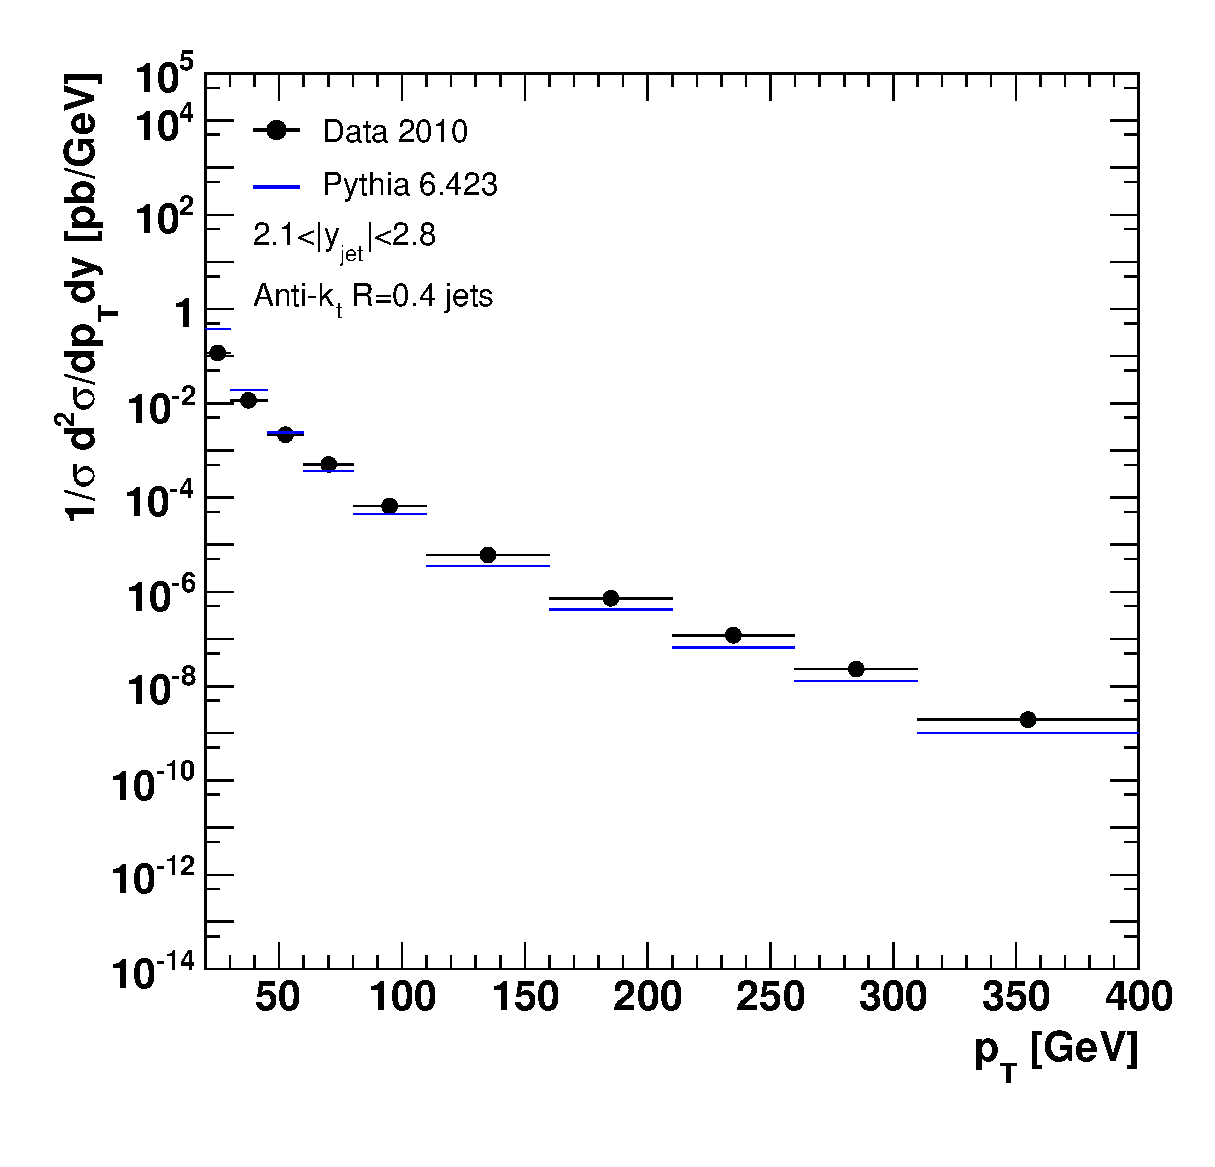
\includegraphics[width=\smallfigwidth]{chapters/forward-inclusive/Control.AntiKt4.2.1y2.8.eps}
    \label{fig:forward-inclusive:akt4_control}}
  \quad
  \subfloat[Data to \MC comparison for \akt $R=0.6$ jets, in the region $3.6 \leq \rap < 4.4$]{
    \includegraphics[width=\smallfigwidth]{chapters/forward-inclusive/Control.AntiKt6.3.6y4.4.eps}
    \label{fig:forward-inclusive:akt6_control}}
  \caption{Control distributions, used to demonstrate the level of agreement between data and \MC; data is shown in black, with \Pythia in blue. \protect\subref{fig:forward-inclusive:akt4_control} shows the comparison for \akt $R=0.4$ jets in the region $2.1 \leq \rap < 2.8$, while \protect\subref{fig:forward-inclusive:akt6_control} shows the comparison for \akt $R=0.6$ jets in the region $3.6 \leq \rap < 4.4$.}
  \label{fig:forward-inclusive:data_mc_control_distributions}
\end{figure}

\section{Systematic Uncertainties}
\label{sec:forward-inclusive:systematics}
Track jets, reconstructed using only information from the tracking detector, are
used to provide an in-situ estimate of jet reconstruction efficiency. The
frequency with which a calorimeter jet was reconstructed, given the existence of
a nearby track jet, was studied in data and \MC and used to infer an uncertainty
on the calorimeter jet reconstruction efficiency measured in \MC. This
disagreement of 1\%, or 2\% for the lowest \pT jets, was taken as a systematic
uncertainty.

The jet energy scale uncertainty, evaluated as described in \SectionRef{sec:analysis-tools:jes_uncertainty},
is the largest single contributor to systematic uncertainties due to the steeply
falling \xs as a function of jet \pT. The JES uncertainty was treated in the same way
as energy resolution, measured from \dijet balancing in data, and
angular resolution, estimated in \MC by matching particle level and detector level
jets; each of these quantities was varied up and down by one standard deviation
and the relative per-bin shift in jet yield was taken as a systematic
uncertainty for that bin. In the central region, $\absRap < 0.8$, the
uncertainty is lower than 4.6\% for all jets with $\pT \geq \unit{20}{\GeV}$, while
for jets with $60 \leq \pT < \unit{800}{\GeV}$ the uncertainty is below 2.5\%, as
can be seen from \FigureRef{fig:analysis-tools:JESUncertainty}.

By propagating these uncertainties through the unfolding procedure, an estimate
of the systematic uncertainty due to unfolding can also be obtained. This is
approximately 5\% at low and high \pT and smaller at intermediate \pT values.
An additional uncertainty of 3.4\% comes from the luminosity measurement.

\begin{figure}[htpb]
  \subfloat[\Akt $R=0.4$ jets, $\absRap < 0.3$]{
    \includegraphics[width=\smallfigwidth]{chapters/forward-inclusive/InclusivePtSysIDS_AntiKt04_00_03.pdf}
    \label{fig:forward-inclusive:uncertainties_akt4}}
  \quad
  \subfloat[\Akt $R=0.6$ jets, $0.8 \leq \absRap < 1.2$]{
    \includegraphics[width=\smallfigwidth]{chapters/forward-inclusive/InclusivePtSysIDS_AntiKt06_08_12.pdf}
    \label{fig:forward-inclusive:uncertainties_akt6}}
  \caption{Summary of relative systematic effects affecting the inclusive jets \xs. \protect\subref{fig:forward-inclusive:uncertainties_akt4} shows the uncertainty for \akt $R=0.4$ jets in the region $\absRap < 0.3$ while \protect\subref{fig:forward-inclusive:uncertainties_akt6} shows the corresponding uncertainty for \akt $R=0.6$ jets in the region $0.8 \leq \absRap < 1.2$. The jet energy scale uncertainty provides the dominant systematic in both cases.}
  \label{fig:forward-inclusive:uncertainties}
\end{figure}

Systematic uncertainties on the final \xs are obtained by summing all
uncertainties in quadrature to give a total uncertainty on the unfolded data; an
example of this process for two \absRap bins can be seen in \FigureRef{fig:forward-inclusive:uncertainties}.
However, the steeply falling jet \pT spectrum, especially at large rapidity,
unavoidably converts even small uncertainties in \pT into large errors on the
measured \xs.

\section{Theoretical Predictions}
\label{sec:forward-inclusive:theory_predictions}
The measured inclusive jet \xs{s} are compared to both NLO \pQCD predictions,
with corrections for non-perturbative effects, and to NLO \MC.

\subsection{Next-to-Leading Order Perturbative \QCD Calculations}
\label{sec:forward-inclusive:NLOpQCD}
Next-to-leading order (NLO) perturbative \QCD (\pQCD) predictions are produced using the \NLOjetpp 4.1.2~\cite{Nagy:2003:NLOjet}
program together with the CT10~\cite{Lai:2010:LHAPDF_CT10} NLO PDFs. The main uncertainties
on the NLO prediction come from the uncertainties on the PDFs, the choice of factorisation
and renormalisation scales (as discussed in \SectionRef{sec:bg-theory:qcd_factorisation})
and the uncertainty in the value of the strong coupling constant, \alphaS.

To estimate the uncertainty on the NLO prediction due to neglected higher-order
terms, each observable was recalculated while varying the renormalisation scale
by a factor of two with respect to the default choice, defined to be the \pT of
the hardest jet in the event. Similarly, to estimate the sensitivity to the choice
of scale where the PDF evolution is separated from the matrix element, the factorisation
scale was separately varied by a factor of two. The experimental uncertainties which
propagate through the PDF fits, together with the associated uncertainties on the
value of $\alphaS(M_Z)$ were used to determine uncertainty bands on the theoretical
predictions; a summary of these corrections can be seen in \FigureRef{fig:forward-inclusive:theory_uncertainties}.
Uncertainties due to the choice of PDF were evaluated by creating predictions using
four different PDF sets and presenting each of these on the final plots.
%The uncertainties due to the choice
%of PDF were evaluated by repeating this calculation using four additional PDFs,
%with the uncertainty on the value of $\alphaS(M_Z)$ established in the same way.
%A summary of these corrections for two sample PDFs can be seen in \FigureRef{fig:forward-inclusive:theory_uncertainties}.

\begin{figure}[htpb]
  \subfloat[\Akt $R=0.4$ jets, $\absRap < 0.3$]{
    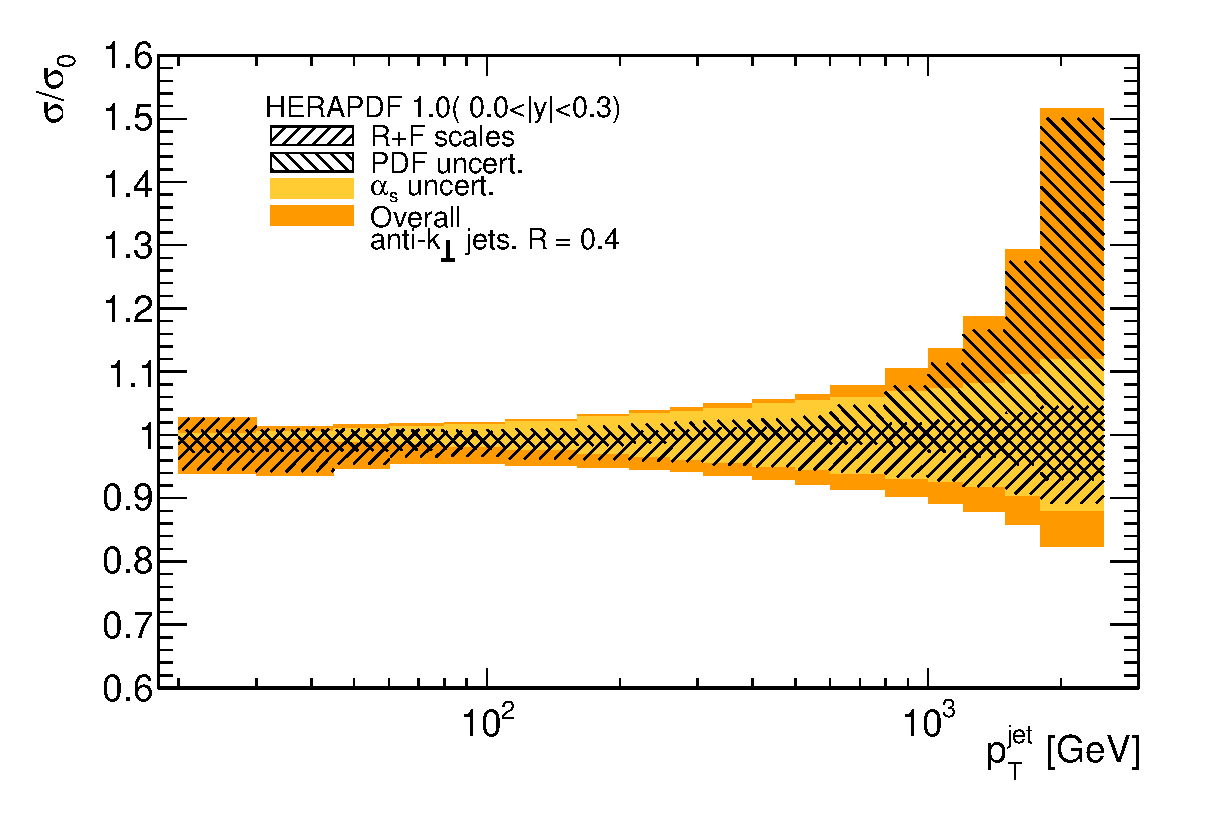
\includegraphics[width=\smallfigwidth]{chapters/forward-inclusive/bands_InclJets04_00_03_HERAPDF10_EIG.eps}
    \label{fig:forward-inclusive:theory_uncertainties_akt4}}
  \quad
  \subfloat[\Akt $R=0.6$ jets, $\absRap < 1.2$]{
    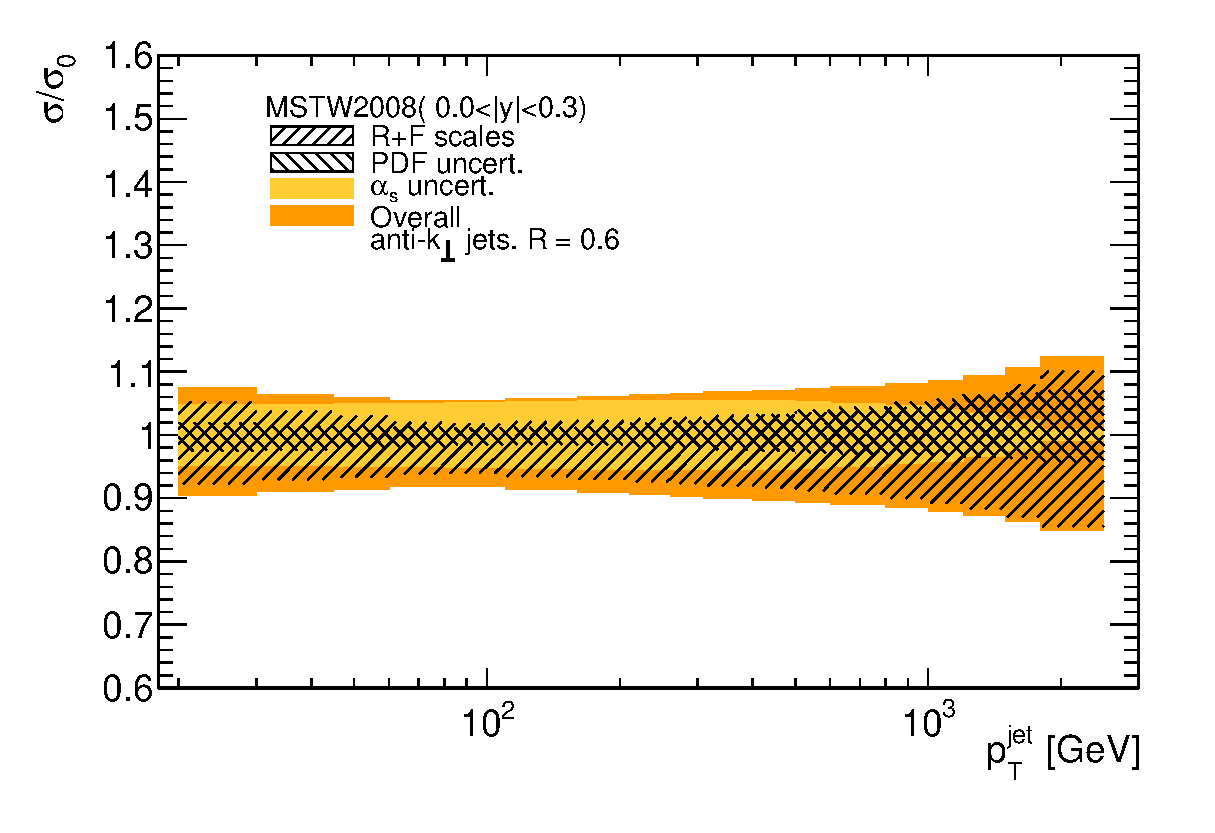
\includegraphics[width=\smallfigwidth]{chapters/forward-inclusive/bands_InclJets06_00_03_MSTW2008nlo90cl.eps}
    \label{fig:forward-inclusive:theory_uncertainties_akt6}}
  \caption{Summary of theory uncertainties arising from the scale choice, uncertainties inherent to the chosen PDF and uncertainties arising from the value of \alphaS. \protect\subref{fig:forward-inclusive:theory_uncertainties_akt4} shows the ratio of the \xs to the nominal \xs for HERAPDF, using \akt $R=0.4$ jets in the region $\absRap < 0.3$ while \protect\subref{fig:forward-inclusive:theory_uncertainties_akt6} shows the same quantity for MSTW2008, using \akt $R=0.6$ jets in the region $\absRap < 0.3$.}
  \label{fig:forward-inclusive:theory_uncertainties}
\end{figure}

Parton level \xs{s}, obtained from fixed-order NLO calculations must be
corrected for non-perturbative effects before they can be compared with data. This
is done by using leading-logarithmic parton shower generators (in this case, \Pythia
with the AUET2B CTEQ6L1 tune~\cite{Pumplin:2002:CTEQ6L1}) to evaluate the ratio of \xs{s} with and without
hadronisation and underlying event. The parton level \xs{s} are then multiplied,
bin-by-bin, by this ratio; tacitly assuming that the effects of soft and hard physics can be
factorised. The uncertainty is estimated as the maximum spread of the correction
factors obtained from performing this procedure using different \Pythia tunes.

\subsection{Next-to-leading Order \MC with Parton Shower}
The \Powheg generator (see \SectionRef{sec:bg-theory:MC:Powheg}) is used to provide
an NLO matrix element prediction. The use of an event generator with NLO matrix elements,
including the simulation of the parton shower, the hadronisation, and the underlying
event, creates a more coherent theoretical prediction and overcomes the need for
separate non-perturbative corrections.

\section{Inclusive Jet \Xs{s}}
The double-differential inclusive jet \xs is shown in \FigureRef{fig:forward-inclusive:InclusiveCrossSectionAKT4}
and \FigureRef{fig:forward-inclusive:InclusiveCrossSectionAKT6} for jets reconstructed
using the \akt algorithm with $R=0.4$ and $R=0.6$ respectively. The measurement
covers the jet \pT range from \unit{20}{\GeV} to \unit{1.5}{\TeV}: spanning two orders
of magnitude in \pT and seven orders of magnitude in \xs. Statistical and
systematic errors on the data are shown, as discussed in \SectionRef{sec:forward-inclusive:systematics},
and the unfolded data is compared to NLO \pQCD predictions which are corrected
for non-perturbative effects as discussed in \SectionRef{sec:forward-inclusive:NLOpQCD}.
It can be seen from \FigureRef{fig:forward-inclusive:NLORatio} that the data and
the theory predictions are generally in good agreement within the experimental and
theoretical uncertainties, with some minor differences visible at high jet \pT and
\absRap.

\begin{figure}
  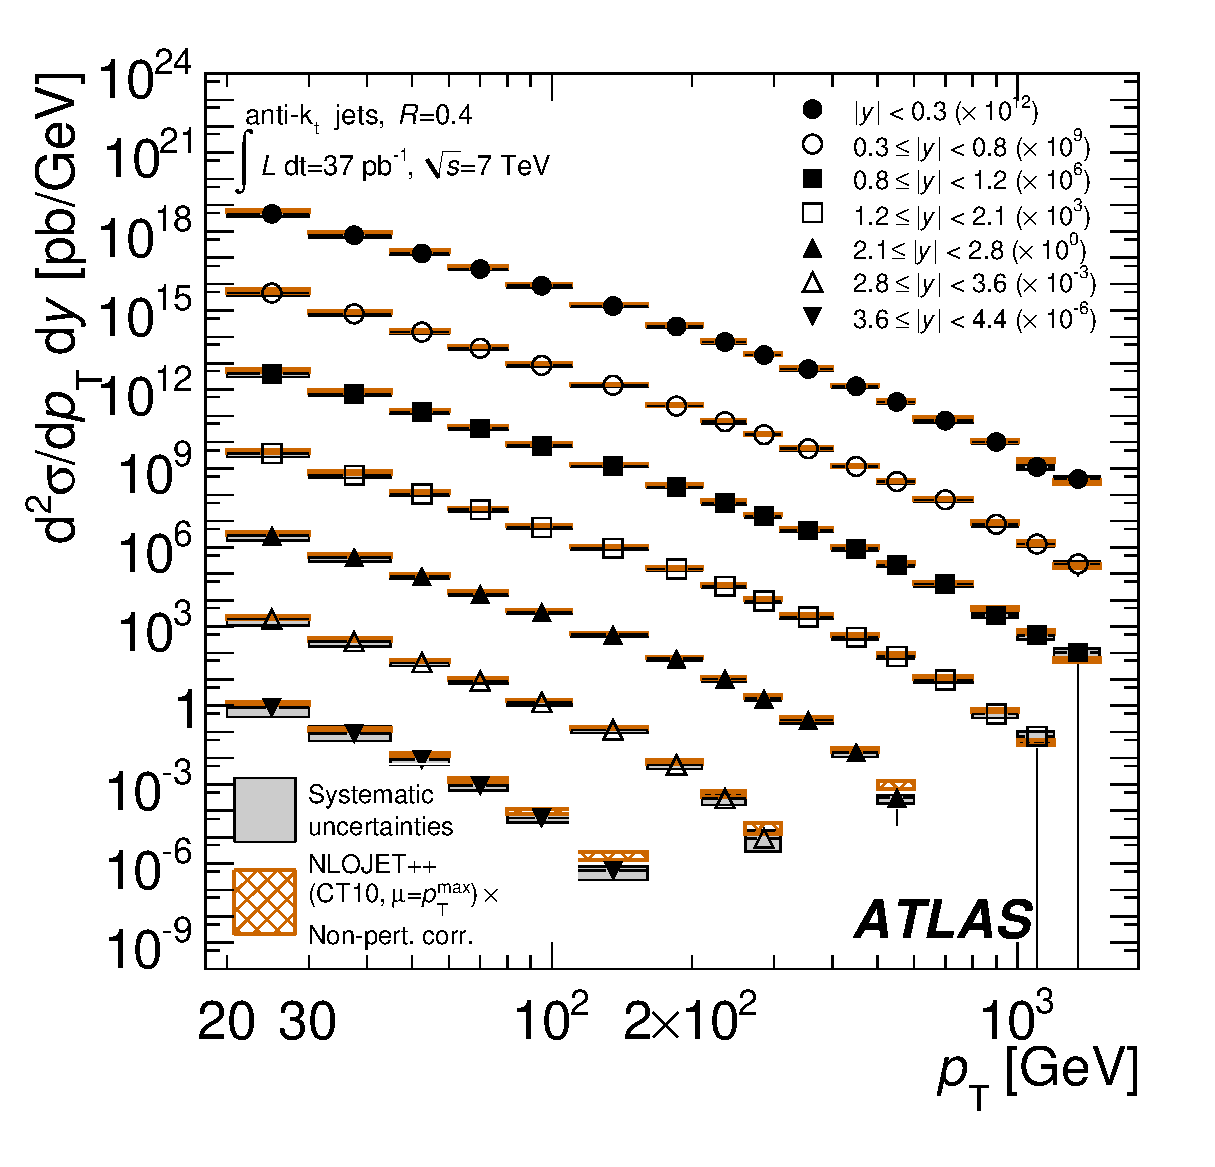
\includegraphics[width=\largefigwidth]{chapters/forward-inclusive/InclusivePtIDS_CT10_AntiKt04.eps}
  \caption{Inclusive jet double-differential \xs as a function of jet \pT in
     different regions of \absRap for jets identified using the \akt algorithm with
     $R=0.4$. For convenience, the \xs{s} are multiplied by the factors indicated
     in the legend. The data are compared to NLO \pQCD calculations to which non-perturbative
     corrections have been applied. The error bars indicate the statistical uncertainty
     on the measurement, and the dark-shaded band indicates the quadratic sum of the
     experimental systematic uncertainties, dominated by the jet energy scale uncertainty.
     There is an additional overall uncertainty of 3.4\% due to the luminosity measurement
     that is not shown. The theory uncertainty (light cross-hatched band) shown is the quadratic
     sum of uncertainties from the choice of renormalisation and factorisation scales,
     parton distribution functions, \alphaS($M_Z$), and the modelling of non-perturbative
     effects, as described in the text.}
  \label{fig:forward-inclusive:InclusiveCrossSectionAKT4}
\end{figure}

\begin{figure}
  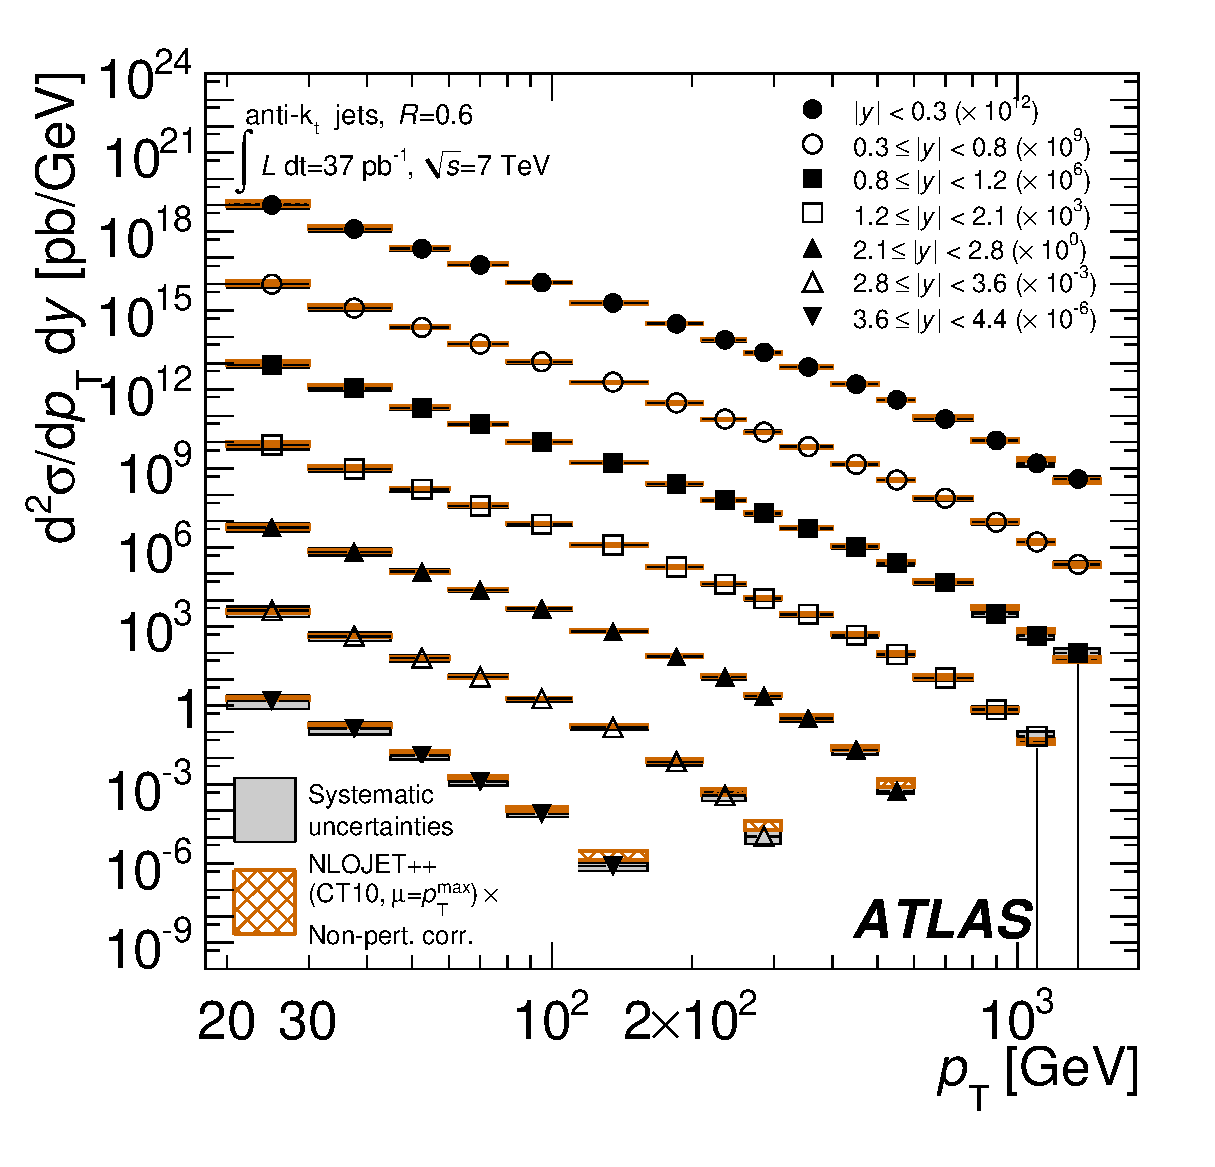
\includegraphics[width=\largefigwidth]{chapters/forward-inclusive/InclusivePtIDS_CT10_AntiKt06.eps}
  \caption{Inclusive jet double-differential \xs as a function of jet \pT in
    different regions of \absRap for jets identified using the \akt algorithm with
    $R=0.6$. For convenience, the \xs{s} are multiplied by the factors indicated
    in the legend. The data are compared to NLO \pQCD calculations to which non-perturbative
    corrections have been applied. The theoretical and experimental uncertainties
    indicated are calculated as described in \FigureRef{fig:forward-inclusive:InclusiveCrossSectionAKT4}.}
  \label{fig:forward-inclusive:InclusiveCrossSectionAKT6}
\end{figure}

\begin{figure}[htpb]
  \subfloat[\Akt $R=0.4$ jets, central rapidities]{
    \includegraphics[width=\smallfigwidth]{chapters/forward-inclusive/InclusivePtIDSRatioCentral_CT10_AntiKt04.eps}
    \label{fig:forward-inclusive:NLORatioCentral_akt4}}
  \quad
  \subfloat[\Akt $R=0.6$ jets, central rapidities]{
    \includegraphics[width=\smallfigwidth]{chapters/forward-inclusive/InclusivePtIDSRatioCentral_CT10_AntiKt06.eps}
    \label{fig:forward-inclusive:NLORatioCentral_akt6}}
  \\
  \subfloat[\Akt $R=0.4$ jets, forward rapidities]{
    \includegraphics[width=\smallfigwidth]{chapters/forward-inclusive/InclusivePtIDSRatioForward_CT10_AntiKt04.eps}
    \label{fig:forward-inclusive:NLORatioForward_akt4}}
  \quad
  \subfloat[\Akt $R=0.6$ jets, forward rapidities]{
    \includegraphics[width=\smallfigwidth]{chapters/forward-inclusive/InclusivePtIDSRatioForward_CT10_AntiKt06.eps}
    \label{fig:forward-inclusive:NLORatioForward_akt6}}
  \caption{Inclusive jet double-differential \xs as a function of jet
           \pT in different regions of \absRap for jets identified using the \akt
           algorithm with $R=0.4$ (left) and $R=0.6$ (right) for central rapidities (top)
           and forward rapidities (bottom). The ratio of the data
           to the theoretical prediction is shown, and the total systematic uncertainties
           on the theory and measurement are indicated. The theoretical and experimental
           uncertainties are calculated as described in \FigureRef{fig:forward-inclusive:InclusiveCrossSectionAKT4}.
           Statistically insignificant data points at large \pT are omitted in this
           ratio.}
  \label{fig:forward-inclusive:NLORatio}
\end{figure}

The comparison of the data with the \Powheg prediction, using the CT10 PDF set, is
shown for \akt jets with $R=0.4$ and $R=0.6$ in different rapidity regions in
\FigureRef{fig:forward-inclusive:PowhegRatio}. Here the data, \Powheg
predictions interfaced either \Pythia (AUET2B and \Perugia~2010 tunes) or \Herwig
(AUET2 tune) as well as fixed order \Powheg with non-perturbative corrections
are all compared. The ratio of each of these is shown with respect to the baseline NLO
\pQCD prediction, again using the CT10 PDF set.

In general, the non-perturbative corrections appear asymmetric here, particularly
at higher values of \pT since the steeply falling \xs means that, when such corrections
are applied, migrations from lower bins to higher predominate over the reverse case.
This results asymmetric shifts with respect to the nominal case, and hence an asymmetric
error band on the ratio.

\Powheg interfaced with \Pythia describes the data better than
when it is interfaced with \Herwig. Since the same matrix element is then passed through
the \Pythia and \Herwig parton showers, it can be deduced that the observable
differences between these predictions must be connected to the specifics of
their parton shower implementations and can be taken as an indication of the
uncertainty arising from the leading-logarithmic approximation used in parton
showering.

It can also be seen that the \Powheg NLO predictions, after parton shower, are in
good agreement with the pure parton level matrix element calculation from \NLOjetpp
after this has been corrected for non-perturbative effects. No direct comparison
has been carried out between the NLO parton level predictions of \Powheg and \NLOjetpp.
This is unlikely to be feasible since the \Powheg formalism guarantees to generate
the hardest third jet in the event while \NLOjetpp only guarantees that a third jet
will be generated. This is also an added complication when interfacing \Powheg with
a parton shower, as a matching process needs to be performed to ensure this condition
is adhered to.

Within the present uncertainties, the \Powheg predictions are consistent with both
the data and \NLOjetpp calculations. There is a trend for \Powheg to predict larger
\xs{s} than both the data and \NLOjetpp at low \pT, and smaller \xs{s} than \NLOjetpp (but
closer to the data) in the high-\pT region. These are also the regions where the
scale uncertainty in \NLOjetpp increases. At low \pT the non-perturbative corrections
have a significant influence, and their uncertainty can be large.

\begin{figure}[htpb]
  \subfloat[\Akt $R=0.4$ jets, central rapidities]{
    \includegraphics[width=\smallfigwidth]{chapters/forward-inclusive/InclusivePtRatioFullPowhegCentral_MSTW2008nlo90cl_AntiKt04.eps}
    \label{fig:forward-inclusive:PowhegRatioCentral_akt4}}
  \quad
  \subfloat[\Akt $R=0.6$ jets, central rapidities]{
    \includegraphics[width=\smallfigwidth]{chapters/forward-inclusive/InclusivePtRatioFullPowhegCentral_MSTW2008nlo90cl_AntiKt06.eps}
    \label{fig:forward-inclusive:PowhegRatioCentral_akt6}}
  \\
  \subfloat[\Akt $R=0.4$ jets, forward rapidities]{
    \includegraphics[width=\smallfigwidth]{chapters/forward-inclusive/InclusivePtRatioFullPowhegForward_MSTW2008nlo90cl_AntiKt04.eps}
    \label{fig:forward-inclusive:PowhegRatioForward_akt4}}
  \quad
  \subfloat[\Akt $R=0.6$ jets, forward rapidities]{
    \includegraphics[width=\smallfigwidth]{chapters/forward-inclusive/InclusivePtRatioFullPowhegForward_MSTW2008nlo90cl_AntiKt06.eps}
    \label{fig:forward-inclusive:PowhegRatioForward_akt6}}
  \caption{Ratios of inclusive jet double-differential \xs to the theoretical
           prediction obtained using \NLOjetpp with the CT10 PDF set. The ratios
           are shown as a function of jet \pT in different regions of \absRap for
           jets identified using the \akt algorithm with $R=0.4$ (left) and
           $R=0.6$ (right) for central rapidities (top) and forward rapidities (bottom).
           The ratios of \Powheg predictions interfaced with
           either \Pythia or \Herwig to the \NLOjetpp predictions corrected for
           non-perturbative effects are shown and can be compared to the corresponding
           ratios for data. Only the statistical uncertainty on the \Powheg predictions
           is shown. The total systematic uncertainties on the theory and the measurement
           are indicated. The \NLOjetpp prediction and the \Powheg ME calculations
           use the CT10 PDF set. Statistically insignificant data points at large \pT
           are omitted in the ratio.}
  \label{fig:forward-inclusive:PowhegRatio}
\end{figure}


\section{Summary}
\label{sec:forward-inclusive:conclusions}
These results represent one of the most comprehensive tests of \QCD ever
performed. Data taken using minimum bias and jet triggers has been combined in
order to measure \xs{s} across a wide range of \pT and rapidity. In particular,
the forward region has never previously been explored with such precision at a
hadron collider.

Jets are reconstructed using the \akt algorithm with $R=0.4$ and $R=0.6$ in
order to probe the relative effects of the parton shower, hadronisation and
underlying event. Overall, the agreement of the NLO perturbative QCD predictions
with the measurements extends over seven orders of magnitude in \xs. These
measurements probe and may constrain the previously unexplored area of parton
distribution functions at large $x$ and high momentum transfer.

In some regions of phase space, the experimental and theoretical uncertainties
are similar in size, thereby providing some sensitivity to different
theoretical predictions. Such differences as have been observed are of the same
order as the NLO scale variation, meaning that no definitive conclusions can yet be drawn. This work has been
published in the European Physical Journal C~\cite{EPJC:2011:ATLASInclusiveJets}
and an updated version has been submitted to Physical Review D~\cite{CERN-PH-EP-2011-192}.

  \chapter{Leading \Dijet \Xs{s}}
\label{chap:dijets}

%\chapterquote{Changing mass consciousness is an individual responsibility.}
%{Dennis Weaver}
%Mass demand has been created almost entirely through the development of advertising.
%{Calvin Coolidge}
\chapterquote{A short reign does not spare the masses.}
{Statius}

\section{Introduction}
As discussed in \ChapterRef{chap:forward-inclusive}, jet \xs measurements are an
important tool for probing theoretical predictions from \QCD. This analysis
examines the leading \dijet \xs as a function of the \dijet mass, \mDijet, in the region
$\yStar < 4.4$, where the variable \yStar is defined as half the rapidity difference
between the two leading (highest \pT) jets, $\yStar = |y_1 - y_2| / 2$, and is the
absolute rapidity of the \dijet{s} in their centre-of-mass frame. The results are
compared to expectations based on next-to-leading order (NLO) \QCD, corrected for
non-perturbative effects, as well as to NLO \MC predictions.

\section{\Xs Definition}
As for the inclusive jet \xs (\SectionRef{sec:forward-inclusive:cross_section_definition}),
the \dijet \xs is defined for the \ATLAS standard jet algorithms: \akt jets with
$R=0.4$ and $R =0.6$. The jet \xs measurements are, again, unfolded back to the
ideal particle level final state of the proton-proton collision. Identically to the
inclusive jet \xs, particle level jets in the \MC are identified with the same
jet algorithms as for data, using all stable particles and hence including muons
and neutrinos from decaying hadrons.

\section{Event Selection}
Similarly to the inclusive jets \xs, events are required to belong to a good run and
to have at least one good primary vertex (see \SectionRef{sec:analysis-tools:data_selection}).
The \dijet pair are selected as the two highest \pT jets in the event, provided
that these satisfy $\pT(j_1) \geq \unit{30}{\GeV}$, $\pT(j_2) \geq \unit{20}{\GeV}$ and
that both jets are within the acceptance region, $\absRap < 4.4$. If either of
these jets are flagged as ``bad'' or ``ugly'' by the standard medium jet
cleaning cuts, as detailed in \SectionRef{sec:analysis-tools:jet_cleaning}, then the event is
discarded. A pair of triggers appropriate to the transverse momentum and rapidity of the \dijet{s}
is then assigned - the event must pass one of these triggers in order to
contribute towards the \xs. Events passing this trigger selection are retained,
with a weight reflecting the amount of luminosity seen by the trigger
combination in question. Approximately 45\% of events passing these cuts contain
at least one additional jet which would also pass the cuts, however, the definition
used here, in which only the leading pair of jets is considered, ensures that there
is no ambiguity in such situations.

\section{Trigger Strategy}
\label{sec:dijets:trigger}
The trigger considerations for \dijet measurements are more complicated than for the
inclusive jet case because the \dijet \xs is measured as a function of the invariant
mass of the two-jet system and the rapidity separation \yStar, while jets are triggered
according to the jet transverse momentum. A per-event strategy based on invariant
mass, only considering events taken by triggers with $>99\%$ efficiency, would force
the use of highly prescaled low-threshold triggers to cover the mass ranges of interest.

The trigger strategy used for the inclusive jet \xs would be inefficient if directly transferred
to the \dijet case since only the two hardest jets in the event are important,
rather than all jets over a given \pT threshold. Similarly, a trigger strategy which
determined a single trigger that the event should pass, based on the \pT of the leading
jet in the event, would unnecessarily lose events due to the effects of prescale.

The strategy adopted is to define two possible trigger chains, based
on the \pT of the two leading jets, and to accept the event if either or both of
these are passed. A similar trigger strategy to that discussed in
\SectionRef{sec:forward-inclusive:trigger} is used: again dependent on the run
period and the \pT and \rap of the two leading jets. One important difference is that
whereas for the single jet \xs, triggers were selected based on whether the
\emph{per-event} efficiency was on plateau, here it must be required that the
\emph{per-jet} efficiency should be on plateau.

Using similar definitions to those discussed in \SectionRef{sec:forward-inclusive:trigger},
the rapidity interval in which jets can be accepted, $\absRap < 4.4$, is divided
into different regions: the central region, $\absRap < 2.9$; the transition region,
$2.9 \leq \absRap < 3.3$; the forward region $3.3 \leq \absRap < 3.6$ and the far-forward
region $3.6 \leq \absRap < 4.4$.

The trigger requirements are summarised in \TableRef{tab:dijets:central_triggers}
for central jets, \TableRef{tab:dijets:forward_triggers} for forward jets
and \TableRef{tab:dijets:far_forward_triggers} for far-forward jets. The transition
region presents additional complications which are discussed in \SectionRef{sec:dijets:transition_region_triggers}.

Having determined the two triggers that each event should pass, based on the \pT
of the two leading jets in the event, it is now required that one or both should have been passed
before the event can be accepted. All events which satisfy this condition are placed
into a trigger category defined by those specific two triggers, in other words,
one trigger category is created for each possible combination of the two triggers.

The equivalent luminosity seen by each trigger category can be calculated (see
\SectionRef{sec:dijets:effective_luminosity}) and the event can then be weighted
by the inverse of this effective luminosity before the final \xs measurements are
produced.

\begin{table}
\begin{center}
  \begin{tabular}{ l l l l l }
    \pT $[\GeV]$ & Run$<$152777 & Periods A--C & Periods D--F  &  Periods G--I       \\
                 &              &              & (minus E1--4) &                     \\
    \midrule
    20--42.5     & L1\_MBTS\_1  & L1\_MBTS\_1  & L1\_MBTS\_1   &  EF\_mbMbts\_1\_eff \\
    42.5--70     & L1\_MBTS\_1  & L1\_J5       & L1\_J5        &  EF\_j20\_jetNoEF   \\
    70--97.5     & L1\_MBTS\_1  & L1\_J15      & L1\_J15       &  EF\_j35\_jetNoEF   \\
    97.5--152.5  & L1\_MBTS\_1  & L1\_J30      & L1\_J30       &  EF\_j50\_jetNoEF   \\
    152.5--197.5 & L1\_MBTS\_1  & L1\_J55      & L1\_J55       &  EF\_j75\_jetNoEF   \\
    197.5--217.5 & L1\_MBTS\_1  & L1\_J55      & L1\_J55       &  EF\_j95\_jetNoEF   \\
    217.5+       & L1\_MBTS\_1  & L1\_J55      & L1\_J55       &  EF\_L1J95\_NoAlg   \\
  \end{tabular}
  \caption{The trigger chains used in the \dijet analysis for the central region, $\absRap<2.9$.}
  \label{tab:dijets:central_triggers}
\end{center}
\end{table}

\begin{table}
\begin{center}
  \begin{tabular}{ l l l l}
    \pT $[\GeV]$ & Periods A--C & Periods E--F  &  Periods G--I         \\
                 &              & (minus E1--4) &                      \\
    \midrule
    20--42.5     & L1\_MBTS\_1  & L1\_MBTS\_1   & EF\_mbMbts\_1\_eff   \\
    42.5--62.5   & L1\_MBTS\_1  & L1\_FJ10      & EF\_mbMbts\_1\_eff   \\
    62.5--72.5   & L1\_MBTS\_1  & L1\_FJ10      & EF\_fj30\_jetNoEF    \\
    72.5--95     & L1\_MBTS\_1  & L1\_FJ30      & EF\_fj30\_jetNoEF    \\
    95--160      & L1\_MBTS\_1  & L1\_FJ30      & EF\_fj50\_jetNoEF    \\
    160+         & L1\_MBTS\_1  & L1\_FJ30      & EF\_fj75\_jetNoEF    \\
  \end{tabular}
  \caption{The trigger chains used in the \dijet analysis for the forward region, $3.3\leq\absRap<3.6$.}
  \label{tab:dijets:forward_triggers}
\end{center}
\end{table}

\begin{table}
\begin{center}
  \begin{tabular}{ l l l l }
    \pT $[\GeV]$ & Periods A--E4 & Periods E5--F &  Periods G--I      \\
                 &               &               &                    \\
    \midrule
    20--42.5     & L1\_MBTS\_1   & L1\_FJ10      & EF\_mbMbts\_1\_eff \\
    42.5--50     & L1\_MBTS\_1   & L1\_FJ10      & EF\_fj30\_jetNoEF  \\
    50--67.5     & L1\_MBTS\_1   & L1\_FJ30      & EF\_fj30\_jetNoEF  \\
    67.5--100    & L1\_MBTS\_1   & L1\_FJ30      & EF\_fj50\_jetNoEF  \\
    100+         & L1\_MBTS\_1   & L1\_FJ30      & EF\_fj75\_jetNoEF  \\
  \end{tabular}
  \caption{The trigger chains used in the \dijet analysis for the far-forward region, $3.6\leq\absRap<4.4$.}
  \label{tab:dijets:far_forward_triggers}
\end{center}
\end{table}

\subsection{Trigger Complications in the Transition Region}
\label{sec:dijets:transition_region_triggers}
As discussed in \SectionRef{sec:forward-inclusive:transition_triggers}, there is
an ambiguity over whether to associate jets which are reconstructed in the transition
region, $2.9 \leq \absRap < 3.3$, with a central or a forward jet trigger. In this
region, which bridges the boundary between the central and forward calorimeters,
rapidity differences between L1 or L2 trigger jets
and offline jets can lead to central trigger jets that are reconstructed offline
as forward jets, and \emph{vice versa}. It can be seen in \FigureRef{fig:forward-inclusive:eta_efficiency_akt}
that the inefficiencies for central and forward triggers overlap by approximately 0.4
in rapidity.

Since each trigger is required to be on a per-jet efficiency plateau, different \pT bin boundaries are used in the central and forward
regions to optimise acceptance; it is, therefore, no longer enough to use a the simple central OR forward logic that could be applied to the
inclusive jet \xs. Accordingly, an angular ``matching'' is performed between offline
jets which fall into this region and trigger objects, to identify the closest trigger
jet and hence whether the offline jet should be classified as central or forward.

\subsubsection{Matching Offline Jets to L1 Triggers}
During periods A--F, when no HLT information was used for event selection,
offline jets must be matched to L1 trigger objects. However, \pseudorap
information is not retained by the FCAL at L1 and so simple \DeltaR matching cannot be
used without risking biases in trigger identification. First the closest \emph{forward} L1 trigger object is identified
as that with the smallest \DeltaPhi with respect to the offline jet. Next the closest
\emph{central} L1 trigger object is identified as that with the smallest \DeltaR
with respect to the offline jet; this takes advantage of the fact that \pseudorap information
is available for L1 objects in the central calorimeter. Having identified the
closest \emph{forward} and the closest \emph{central} L1 objects, whichever one
has the smaller \DeltaPhi separation with respect to the offline jet is assigned
as the best match.

\subsubsection{Matching Offline Jets to L2 Triggers}
In contrast to L1 objects, L2 trigger jets have \pseudorap information in all calorimeter
systems. For periods G--I therefore, when the HLT was in rejection mode, each offline
jet can be matched to the L2 trigger jet that is closest to it in \DeltaR; in other
words, the trigger jet that has the smallest \DeltaR with respect to the offline jet.
Since each L2 trigger jet is seeded by a L1 ROI, it can be uniquely determined whether
the L2 jet was seeded from a central or forward L1 ROI and hence whether the offline
jet should be associated with a central or forward trigger.

This procedure makes optimal use of such angular information as is available, avoiding
bias by using \DeltaPhi to discriminate among forward L1 ROIs, where \DeltaR would
tend to incorrectly assign forward jets as central. However it still takes advantage of
the \pseudorap information where possible in order to discriminate between central
L1 trigger jets.

\subsubsection{Determining \DeltaR and \DeltaPhi for Matching}
\label{sec:dijets:matching}
The matching procedures described above are subject to the constraint that an offline
jet is considered to be matched to a trigger jet only if they are separated by less
than a maximum value of $\DeltaR < 0.5$ or $\DeltaPhi < 0.4$, depending which metric
is used. The value of the maximum \DeltaR allowed for a match was chosen by inspecting
the \DeltaR distribution of the closest trigger jet, which is shown in
\FigureRef{fig:dijets:DeltaR}. The distribution has a Gaussian core that extends
to approximately $\DeltaR \simeq 0.5$. This Gaussian population indicates a genuine
correspondence between the offline jet and the closest trigger jet, where the smearing
arises from the fundamentally different way in which offline and trigger jets are constructed.
However, beyond this, in the region $\DeltaR > 0.5$, a large non-Gaussian tail dominates.
The non-Gaussian behaviour of this population indicates that these are mismatches,
and that the offline jet and its closest trigger jet in fact have no real association.
The boundary between these two populations occurring at $\DeltaR=0.5$ thus distinguishes
between real matches and mismatches, so it is the optimal value for the \DeltaR
matching cut.

A similar analysis was performed for the \DeltaPhi distribution shown
in \FigureRef{fig:dijets:DeltaPhi} in order to derive the optimal matching cut of
$\DeltaPhi < 0.4$. In both the \DeltaR and \DeltaPhi cases, the studies were performed
outside the region of interest, looking separately at more central jets, with $2.3 \leq \absRap < 2.9$
and more forward jets, with $3.3 \leq \absRap < 3.9$. This was done in order to
ensure that the choice of cut was not biased by inefficiencies in triggering that
would be present in the transition region. The distributions show a noticeable dependence
on the \pT region considered, with the lowest \pT region showing a large number of
events in which the best matched trigger jet is a large distance away from the offline
jet; this effect is an artefact of the low \pT offline jets considered
here. The low edge of the \pT bins used for this study is not yet on the efficiency plateau of the
relevant triggers, and so there will be cases in which a real offline jet has no
counterpart among the collection of trigger jets. In such cases, the closest matched
trigger jet will necessarily be an uncorrelated object which may therefore be a large
distance away. Since the jets used in the analysis are always on their trigger plateau
this is not an issue for the measurement. In fact the percentage of jets which are
rejected by this matching procedure as a result of the closest match being above the
cut is of the order of 0.5\%, depending on \pT, and a systematic error is assigned
to account for this.

\begin{figure}[htpb]
  \subfloat[L1 central jets]{
    \includegraphics[width=\tinyfigwidth]{chapters/dijets/dR_L1j24_29.eps}
    \label{fig:dijets:dR_L1j24_29}}
  \quad
  \subfloat[L2 central jets]{
    \includegraphics[width=\tinyfigwidth]{chapters/dijets/dR_L2j24_29.eps}
    \label{fig:dijets:dR_L2j24_29}}
  \quad
  \subfloat[L2 forward jets]{
    \includegraphics[width=\tinyfigwidth]{chapters/dijets/dR_L2fj34_39.eps}
    \label{fig:dijets:dR_L2fj34_39}}
  \caption{Angular separation \DeltaR between an offline jet and the closest trigger jet at L1 and L2. \protect\subref{fig:dijets:dR_L1j24_29} L1 central jets, \protect\subref{fig:dijets:dR_L2j24_29} L2 central jets and \protect\subref{fig:dijets:dR_L2fj34_39} are shown separately. The distribution is not shown for the forward region at L1 since the FCAL has no \pseudorap measurement at L1. The distributions indicate that the optimal \DeltaR cut to distinguish real matches from mismatches is $\DeltaR < 0.5$.}
  \label{fig:dijets:DeltaR}
\end{figure}

\begin{figure}[htpb]
  \subfloat[L1 central jets]{
    \includegraphics[width=\smallfigwidth]{chapters/dijets/dPhi_L1j24_29.eps}
    \label{fig:dijets:dPhi_L1j24_29}}
  \quad
  \subfloat[L1 forward jets]{
    \includegraphics[width=\smallfigwidth]{chapters/dijets/dPhi_L1fj34_39.eps}
    \label{fig:dijets:dPhi_L1fj24_29}}
  \\
  \subfloat[L2 central jets]{
    \includegraphics[width=\smallfigwidth]{chapters/dijets/dPhi_L2j24_29.eps}
    \label{fig:dijets:dPhi_L2j24_29}}
  \quad
  \subfloat[L2 forward jets]{
    \includegraphics[width=\smallfigwidth]{chapters/dijets/dPhi_L2fj34_39.eps}
    \label{fig:dijets:dPhi_L2fj34_39}}
  \caption{Angular separation \DeltaPhi between an offline jet and the closest trigger
           jet at L1 (top) and L2 (bottom) for central jets (left) and forward jets
           (right). The distributions indicate that the optimal
           \DeltaPhi cut to distinguish real matches from mismatches is $\DeltaPhi < 0.4$.}
  \label{fig:dijets:DeltaPhi}
\end{figure}


\subsection{Per-Jet Trigger Inefficiencies}
Unlike the case of the inclusive jet efficiency, there is a ``crack'' region between
the calorimeter barrel and end-cap regions ($1.3 \leq \absRap \leq 1.6$) where the
per-jet trigger efficiency never becomes fully efficient due to calorimeter inhomogeneities.
The per-jet trigger efficiency in this crack region is shown in Table~\ref{tab:dijets:crack_efficiency}.

Additionally, due to a dead FCAL trigger tower that spans a width of $\Delta \phi=\pi/4$ in the
rapidity region $\eta>3.1$, the forward jet triggers are not fully efficient in
this region.  The per-jet efficiency is shown for the rapidity region $3.1 \leq \absRap < 3.6$
in \TableRef{tab:dijets:transition_efficiency} and for the forward region $3.6 \leq \absRap < 4.4$
in \TableRef{tab:dijets:forward_efficiency}.

A trigger efficiency correction is applied to any of the \dijet{s} that fall into either of these regions; in each case, the jet is weighted by the inverse of its trigger efficiency.
A systematic error is assigned for this procedure, equal to the maximal correction.

\begin{table}
\begin{center}
  \begin{tabular}{ l c c c }
    \pT $[\GeV]$ & Run$<152777$ & Run 152777--Period F & Period G--I \\
    \midrule
    20--42.5     & 1.00         & 1.00                 & 1.00       \\
    42.5--70     & 1.00         & 0.89                 & 0.96       \\
    70--97.5     & 1.00         & 0.88                 & 0.87       \\
    97.5--152.5  & 1.00         & 0.81                 & 0.83       \\
    152.5--197.5 & 1.00         & 0.83                 & 0.82       \\
    197.5--217.5 & 1.00         & 0.83                 & 0.80       \\
    217.5+       & 1.00         & 0.83                 & 0.81       \\
   \end{tabular}
  \caption{The plateau per-jet trigger efficiency in the crack region $1.3 \leq \absRap < 1.6$.
           Trigger inefficiency arises due to inhomogeneities in the crack region
           and is corrected for in the \dijet measurement.}
  \label{tab:dijets:crack_efficiency}
\end{center}
\end{table}

\begin{table}
\begin{center}
  \begin{tabular}{ l c c c }
    \pT $[\GeV]$ & Periods A--D & Periods E--F  & Period G--I \\
                 &              & (minus E1--4) &              \\
    \midrule
    20--42.5     & 1.00         & 1.00          & 1.00       \\
    42.5--62.5   & 1.00         & 1.00          & 1.00       \\
    62.5--72.5   & 1.00         & 1.00          & 0.99       \\
    72.5--95     & 1.00         & 0.97          & 0.99       \\
    95--160      & 1.00         & 0.97          & 0.99       \\
    160+         & 1.00         & 0.97          & 1.00       \\
   \end{tabular}
  \caption{The per-jet trigger efficiency for the jet rapidity region $3.1 \leq \absRap < 3.6$.
           Trigger inefficiency arises due to the dead FCAL tower and is corrected
           for in the \dijet measurement.}
  \label{tab:dijets:transition_efficiency}
\end{center}
\end{table}

\begin{table}
\begin{center}
  \begin{tabular}{ l c c c }
    \pT $[\GeV]$ & Periods A--D & Periods E--F  & Period G--I \\
                 &              & (minus E1--4) &             \\
    \midrule
    20--42.5     & 1.00         & 0.95          & 1.00        \\
    42.5--50     & 1.00         & 0.95          & 0.99        \\
    50--67.5     & 1.00         & 0.95          & 0.99        \\
    67.5--100    & 1.00         & 0.95          & 0.97        \\
    100+         & 1.00         & 0.95          & 0.97        \\
   \end{tabular}
  \caption{The per-jet trigger efficiency for the jet rapidity region $3.6 \leq \absRap < 4.4$.
           Trigger inefficiency arises due to the dead FCAL tower and is corrected
           for in the \dijet measurement.}
  \label{tab:dijets:forward_efficiency}
\end{center}
\end{table}

\subsection{Calculating Effective Luminosity}
\label{sec:dijets:effective_luminosity}
In \SectionRef{sec:forward-inclusive:transition_triggers} it was possible to determine
a \xs for the case in which multiple triggers were used by dividing events up according
to which triggers they would have passed before prescale. Here, however, the number
of trigger categories is large and hence it would be preferable not to divide up the number
of events any further.

Given that the triggers are selected in such a way that they are on plateau in the
relevant region, it is expected that, in the absence of efficiency or prescale
effects, all events should pass both of the appropriate triggers. Defining the case where the leading
jet passes its trigger as $T_{10}$ and the case where the second jet passes its trigger
as $T_{01}$, this would mean that all events belong to case $T_{11}$.

In the hypothetical case where the leading and second jet triggers had respective
prescales $P^{\mathrm{L}}$ and $P^{\mathrm{S}}$ but no inefficiencies, some events would
move to $T_{10}$, some to $T_{01}$ and some to $T_{00}$. The effective luminosity
for the events remaining in one of $T_{10}$, $T_{01}$ and $T_{11}$ would be,
after summing over all luminosity blocks, LB:

\begin{equation}
  \mathcal{L}_{\mathrm{effective}} = \sum_{\mathrm{LB}} \frac{\mathcal{L}_{\mathrm{LB}}}{P^{\mathrm{L}}_{\mathrm{LB}} P^{\mathrm{S}}_{\mathrm{LB}}/(P^{\mathrm{L}}_{\mathrm{LB}} + P^{\mathrm{S}}_{\mathrm{LB}}-1)}
\end{equation}

\noindent where $\mathcal{L}_{\mathrm{LB}}$ is the luminosity of each luminosity block.
This is simply the degenerate case of \EquationRef{eq:forward-inclusive:final_luminosity}
in which all events belong to the last category. Unlike that situation, however,
it is no longer important which events belong to which category before prescale: an
identical effective luminosity can be applied to all events in the trigger category.

With the addition of trigger inefficiencies, the situation becomes slightly more
complicated. However, after compensating for inefficiency, only the total number
of events needs to be determined. It can be demonstrated, see \AppendixRef{chap:appendix:trigger_efficiencies},
that, if events are weighted as shown in \TableRef{tab:dijets:efficiency_correction}, then this total
number of events can be correctly recovered: although the individual
numbers no longer directly indicate which triggers were passed, the total number
passing one of the two triggers is correct.

\begin{table}
\begin{center}
  \begin{tabular}{ l l }
    Triggers passed (after prescale) & Efficiency weighting          \\
    \midrule
    Leading jet ($T_{10}$)           & $1/e_L$                       \\
    Second jet ($T_{01}$)            & $1/e_S$                       \\
    Both triggers ($T_{11}$)         & $1/e_L + 1/e_S - 1/(e_L*e_S)$ \\
   \end{tabular}
  \caption{The efficiency weightings for different combinations of passed triggers.
           $e_L$ is the efficiency of the leading jet trigger and $e_S$ is the efficiency
           of the second jet trigger.}
  \label{tab:dijets:efficiency_correction}
\end{center}
\end{table}

\section{Validating the Two-Trigger Strategy}
This trigger procedure was validated to ensure that it gave compatible results with
a simpler single-trigger strategy. Additionally, investigations were made to determine
optimum values for the matching cuts, which are discussed in \SectionRef{sec:dijets:matching}.
Finally a closure test was performed with \MC, where the effects of the trigger
have been emulated using the prescale values of a typical run.

The implementation of this method is validated using a closure test with Monte
Carlo, where the effects of the trigger are emulated using the prescale values
of a typical run. \MC events are discarded at random according to the prescales
of the triggers appropriate to the \dijet pair, with the surviving events constituting
a ``triggered pseudodata'' sample, which is then analysed with the same procedure as is used
for data. In particular, the pseudo-triggered events are assigned to trigger categories, the
\dijet mass histogram from each trigger category is divided by the appropriate
equivalent luminosity, and finally the resulting \xs{s} from all the trigger categories
are combined to obtain the final detector level results.

The resulting \dijet mass spectrum in slices of the rapidity separation \yStar from
0.0 to 4.4 is shown in \FigureRef{fig:dijets:closure} for both the pseudo-triggered and untriggered
\MC samples. The distributions obtained after trigger emulation and correction using the trigger
analysis code are compatible, within the available statistics, with the same distributions from the original
\MC sample without the trigger requirement, hence validating the two-jet trigger method.

\begin{figure}[htpb]
  \subfloat[\Dijet closure $0.0 \leq \yStar < 4.4$]{
    \includegraphics[width=\smallfigwidth]{chapters/dijets/DijetClosure.AntiKt6.yStar.eps}
    \label{fig:dijets:closure_all}}
  \quad
  \subfloat[\Dijet closure, $1.0 \leq \yStar < 1.5$]{
    \includegraphics[width=\smallfigwidth]{chapters/dijets/DijetClosure.AntiKt6.yStar1.0_1.5.eps} %DijetClosure.AntiKt6.yStar1.5_2.0.eps}
    \label{fig:dijets:closure_ratio}}
  \caption{Summary of the closure test for a \dijet \MC sample for jets identified using the \akt algorithm with $R=0.6$. The black dots represent the result of emulating the trigger in the \MC and then correcting for it using the same technique used on data (the pseudodata sample), while the blue solid lines (overlaid) represent the result of analysing all events, without trigger corrections (the \MC sample). The results are presented in \protect\subref{fig:dijets:closure_all} as a function of \mDijet in different \yStar bins while in \protect\subref{fig:dijets:closure_ratio} the case $1.0 \leq \yStar < 1.5$ is shown separately, together with the ratio of pseudodata to \MC in each mass bin.}
  \label{fig:dijets:closure}
\end{figure}

\section{Effective Luminosities}
For the \dijet measurements, the luminosities are calculated for the two-jet trigger
scheme used (see \TableRangeRef{tab:dijets:central_triggers}{tab:dijets:far_forward_triggers}).
The effective luminosities for different trigger combinations
are shown for Periods A--D in \TableRef{tab:dijets:LumiDijetPeriodAD}, for Periods E5--F
in \TableRef{tab:dijets:LumiDijetPeriodE5F}, and for Periods G--I in \TableRef{tab:dijets:LumiDijetPeriodGI}.

\begin{table}
\begin{center}
  \begin{tabular}{ r r@{.}l r@{.}l r@{.}l r@{.}l r@{.}l }
                & \multicolumn{2}{l}{L1\_MBTS\_1} & \multicolumn{2}{l}{L1\_J5}  & \multicolumn{2}{l}{L1\_J15} & \multicolumn{2}{l}{L1\_J30} & \multicolumn{2}{l}{L1\_J55} \\
    \cmidrule{2-11}
    L1\_MBTS\_1 & 0&0005827                       & 0&02627                     & 0&2723                      & 0&2723                      & 0&2723                      \\
    L1\_J5      & \multicolumn{2}{l}{}            & 0&2723                      & 0&2723                      & 0&2723                      & 0&2723                      \\
    L1\_J15     & \multicolumn{2}{l}{}            & \multicolumn{2}{l}{}        & 0&2723                      & 0&2723                      & 0&2723                      \\
    L1\_J30     & \multicolumn{2}{l}{}            & \multicolumn{2}{l}{}        & \multicolumn{2}{l}{}        & 0&2723                      & 0&2723                      \\
    L1\_J55     & \multicolumn{2}{l}{}            & \multicolumn{2}{l}{}        & \multicolumn{2}{l}{}        & \multicolumn{2}{l}{}        & 0&2723                      \\
  \end{tabular}
  \caption{Effective luminosity in \ipb of different trigger combinations used in
           Periods A--D.}
  \label{tab:dijets:LumiDijetPeriodAD}
\end{center}
\end{table}

\begin{table}
\begin{center}
  \begin{tabular}{ r r@{.}l r@{.}l r@{.}l r@{.}l }
                & \multicolumn{2}{l}{L1\_MBTS\_1} & \multicolumn{2}{l}{L1\_J5}   & \multicolumn{2}{l}{L1\_J15}  & \multicolumn{2}{l}{L1\_J30} \\
    \cmidrule{2-9}
    L1\_MBTS\_1 & 0&00008220                      & 0&002549                     & 0&02488                      & 1&136                       \\
    L1\_J5      & \multicolumn{2}{l}{}            & 0&002473                     & 0&02728                      & 1&137                       \\
    L1\_J15     & \multicolumn{2}{l}{}            & \multicolumn{2}{l}{}         & 0&02489                      & 1&140                       \\
    L1\_J30     & \multicolumn{2}{l}{}            & \multicolumn{2}{l}{}         & \multicolumn{2}{l}{}         & 1&136                       \\
                & \multicolumn{2}{l}{L1\_J55}     & \multicolumn{2}{l}{L1\_FJ10} & \multicolumn{2}{l}{L1\_FJ30} & \multicolumn{2}{l}{}        \\
    \cmidrule{2-9}
    L1\_MBTS\_1 & 2&251                           & 0&01606                      & 2&251                        & \multicolumn{2}{l}{}        \\
    L1\_J5      & 2&251                           & 0&01844                      & 2&251                        & \multicolumn{2}{l}{}        \\
    L1\_J15     & 2&251                           & 0&04019                      & 2&251                        & \multicolumn{2}{l}{}        \\
    L1\_J30     & 2&251                           & 1&137                        & 2&251                        & \multicolumn{2}{l}{}        \\
    L1\_J55     & 2&251                           & 2&251                        & 2&251                        & \multicolumn{2}{l}{}        \\
    L1\_FJ10    & \multicolumn{2}{l}{}            & 0&01600                      & 2&251                        & \multicolumn{2}{l}{}        \\
    L1\_FJ30    & \multicolumn{2}{l}{}            & \multicolumn{2}{l}{}         & 2&251                        & \multicolumn{2}{l}{}        \\
  \end{tabular}
  \caption{Effective luminosity in \ipb of different trigger combinations used in
           Periods E5--F.}
  \label{tab:dijets:LumiDijetPeriodE5F}
\end{center}
\end{table}

\begin{table}
\begin{center}
  \begin{tabular}{ r r@{.}l r@{.}l r@{.}l r@{.}l }
                   & \multicolumn{2}{l}{mbMbts\_1\_eff} & \multicolumn{2}{l}{j20\_jetNoEF}  & \multicolumn{2}{l}{j35\_jetNoEF}  & \multicolumn{2}{l}{j50\_jetNoEF}  \\
    \cmidrule{2-9}
    mbMbts\_1\_eff & 0&0001021                          & 0&002504                          & 0&05213                           & 0&2541                            \\
    j20\_jetNoEF   & \multicolumn{2}{l}{}               & 0&002418                          & 0&05437                           & 0&2578                            \\
    j35\_jetNoEF   & \multicolumn{2}{l}{}               & \multicolumn{2}{l}{}              & 0&05203                           & 0&2782                            \\
    j50\_jetNoEF   & \multicolumn{2}{l}{}               & \multicolumn{2}{l}{}              & \multicolumn{2}{l}{}              & 0&2556                            \\
                   & \multicolumn{2}{l}{j75\_jetNoEF}   & \multicolumn{2}{l}{fj30\_jetNoEF} & \multicolumn{2}{l}{fj50\_jetNoEF} & \multicolumn{2}{l}{fj75\_jetNoEF} \\
    \cmidrule{2-9}
    mbMbts\_1\_eff & 6&507                              & 0&1643                            & 3&871                             & 35&69                             \\
    j20\_jetNoEF   & 6&508                              & 0&1665                            & 3&873                             & 35&69                             \\
    j35\_jetNoEF   & 6&521                              & 0&1891                            & 3&889                             & 35&69                             \\
    j50\_jetNoEF   & 6&569                              & 0&3424                            & 3&951                             & 35&69                             \\
    j75\_jetNoEF   & 6&507                              & 6&558                             & 7&906                             & 35&69                             \\
    fj30\_jetNoEF  & \multicolumn{2}{l}{}               & 0&1642                            & 3&937                             & 35&69                             \\
    fj50\_jetNoEF  & \multicolumn{2}{l}{}               & \multicolumn{2}{l}{}              & 3&871                             & 35&69                             \\
    fj75\_jetNoEF  & \multicolumn{2}{l}{}               & \multicolumn{2}{l}{}              & \multicolumn{2}{l}{}              & 35&69                             \\
  \end{tabular}
  \caption{Effective luminosity in \ipb of different trigger combinations used in
           Periods G--I. The initial ``EF\_'' has been left off all trigger names
           for brevity.}
  \label{tab:dijets:LumiDijetPeriodGI}
\end{center}
\end{table}

\section{Unfolding Detector Effects}
Unfolding of the \dijet \xs{s} is performed using the IDS method as described
in \SectionRef{sec:forward-inclusive:unfolding}. The same binning is used as for
the final distributions and the particle level spectra in \MC are reweighted to
correct for any shape mismodelling as discussed previously.

\FigureRef{fig:dijets:data_mc_control_distributions} shows the level of agreement
between \Pythia and the data for two sample distributions; an event-by-event reweighting
function is calculated and applied to the particle level spectra in \MC to eliminate
any effects of shape differences between data and \MC.

\begin{figure}[htpb]
  \subfloat[Data to \MC comparison for \akt $R=0.4$, in the region $0.5 \leq \yStar < 1.0$]{
    \includegraphics[width=\smallfigwidth]{chapters/dijets/Control.InclusiveDijets.AntiKt4.yStar0.5_1.eps}
    \label{fig:dijets:control_akt4_05_1}}
  \quad
  \subfloat[Data to \MC comparison for \akt $R=0.6$, in the region $2.0 \leq \yStar < 2.5$]{
    \includegraphics[width=\smallfigwidth]{chapters/dijets/Control.InclusiveDijets.AntiKt6.yStar2_2.5.eps}
    \label{fig:dijets:control_akt6_2_25}}
  \caption{Control distributions, used to demonstrate the level of agreement between data and \MC. Data is shown in black, with \Pythia in blue. \protect\subref{fig:dijets:control_akt4_05_1} shows the comparison for \akt $R=0.4$ jets in the region $0.5 \leq \yStar < 1.0$, while \protect\subref{fig:dijets:control_akt6_2_25} shows the comparison for \akt $R=0.6$ jets in the region $2.0 \leq \yStar < 2.5$.}
  \label{fig:dijets:data_mc_control_distributions}
\end{figure}

\section{Systematic Uncertainties}
The systematic uncertainties for the \dijet \xs measurements are calculated,
propagated and combined as described in \SectionRef{sec:forward-inclusive:systematics}.
The jet energy scale uncertainty is again the largest single contributor to the
overall uncertainty, dominating the other contributions, particularly in the
high mass region when the \xs is steeply falling.

\section{Theoretical Predictions}
Measured \dijet \xs{s} are compared to both NLO \pQCD predictions,
with corrections for non-perturbative effects, and to NLO \MC. The NLO
\pQCD predictions are produced using \NLOjetpp 4.1.2~\cite{Nagy:2003:NLOjet}
with the CT10~\cite{Lai:2010:LHAPDF_CT10} NLO PDFs while NLO \MC predictions
come from \Powheg, interfaced with both \Pythia and \Herwig. Uncertainties are
determined as outlined in \SectionRef{sec:forward-inclusive:theory_predictions}.

\section{Leading \Dijet \Xs{s}}
The \dijet double-differential \xs is measured as a function of the \dijet
invariant mass for nine bins of the variable \yStar, defined as
half the absolute value of the rapidity difference of the two leading jets, ranging
from 0 to 4.4. The results are shown in \FiguresRef{fig:dijets:InclusiveCrossSectionAKT4}{fig:dijets:InclusiveCrossSectionAKT6} for \akt jets with $R=0.4$
and $R=0.6$, respectively. The \xs falls rapidly with mass, and extends up to \dijet
masses of nearly \unit{5}{\TeV}.

\begin{figure}
  \includegraphics[width=\largefigwidth]{chapters/dijets/DijetMassYStarNLO_04.eps}
  \caption{\Dijet double-differential \xs as a function of \dijet mass, binned
     in half the rapidity separation between the two leading jets, $\yStar = |y_1 - y_2|/2$,
     for jets identified using the \akt algorithm with $R=0.4$. For convenience,
     the \xs{s} are multiplied by the factors indicated in the legend. The
     data are compared to NLO \pQCD calculations from \NLOjetpp, using the CT10
     PDF set and to which non-perturbative corrections have been applied. The error
     bars, which are usually smaller than the symbols, indicate the statistical
     uncertainty on the measurement. The dark-shaded band indicates the quadratic
     sum of the experimental systematic uncertainties, which are dominated by
     the jet energy scale uncertainty. There is an additional overall uncertainty
     of 3.4\% due to the luminosity measurement that is not shown. The theory uncertainty,
     shown as the light cross-hatched band, is the quadratic sum of uncertainties
     from the choice of the renormalisation and factorisation scales, PDFs, $\alphaS(M_Z)$,
     and the modelling of non-perturbative effects, as described in the text.}
  \label{fig:dijets:InclusiveCrossSectionAKT4}
\end{figure}


\begin{figure}
  \includegraphics[width=\largefigwidth]{chapters/dijets/DijetMassYStarNLO_06.eps}
  \caption{\Dijet double-differential \xs as a function of \dijet mass, binned
     in half the rapidity separation between the two leading jets, $\yStar = |y_1 - y_2|/2$,
     for jets identified using the \akt algorithm with $R=0.6$. For convenience,
     the \xs{s} are multiplied by the factors indicated in the legend. The
     data are compared to NLO \pQCD calculations from \NLOjetpp, using the CT10
     PDF set and to which non-perturbative corrections have been applied. The systematic
     uncertainties are calculated as described in \FigureRef{fig:dijets:InclusiveCrossSectionAKT4}.}
  \label{fig:dijets:InclusiveCrossSectionAKT6}
\end{figure}

The comparison of the data with the \Powheg prediction, using the CT10 PDF set,
is shown in different \yStar regions in \FiguresRef{fig:dijets:PowhegRatio_akt4_central}{fig:dijets:PowhegRatio_akt4_forward}
for \akt jets with $R=0.4$ and in \FiguresRef{fig:dijets:PowhegRatio_akt6_central}{fig:dijets:PowhegRatio_akt6_forward}
for \akt jets with $R=0.6$. Here the data, \Powheg predictions interfaced with
\Pythia (AUET2B and \Perugia~2010 tunes) and \Herwig (AUET2 tune) and fixed order
\Powheg with non-perturbative corrections are all compared. The ratio of each of
these with respect to the NLO pQCD prediction (CT10 PDF set) baseline is shown.

As in the inclusive jets case, the \Powheg prediction agrees better with data
after being interfaced with \Pythia than with \Herwig. Since the same matrix
element, which agrees with the \NLOjetpp prediction, is used in both cases, this
provides further evidence that the \Pythia parton shower approach more
accurately reproduces the data than the angle-ordered parton shower used by
\Herwig. The \Perugia tune of \Pythia also performs badly, but this is a deliberately
extreme tune, which is not expected to agree well with the data. In general, the
\Herwig tunes used for these comparisons are perhaps not correctly optimised for
\LHC data - additional tunes may provide improved agreement in future.

%\begin{figure}[htbp]
%  \subfloat[\Akt $R=0.4$, small \yStar]{
%    \includegraphics[width=\smallfigwidth]{chapters/dijets/DijetMassYStarRatioFinal04_central.eps}
%    \label{fig:dijets:PowhegRatioSmallYStar_akt4}}
%  \quad
%  \subfloat[\Akt $R=0.6$, small \yStar]{
%    \includegraphics[width=\smallfigwidth]{chapters/dijets/DijetMassYStarRatioFinal06_central.eps}
%    \label{fig:dijets:PowhegRatioSmallYStar_akt6}}
%  \caption{Ratios of inclusive \dijet double-differential \xs to the theoretical
%           prediction obtained using \NLOjetpp with the CT10 PDF set. The ratios
%           are shown as a function of \dijet mass, binned in half the rapidity separation
%           between the two leading jets, $\yStar = |y_1 - y_2|/2$, for $0.0 \leq \yStar < 2.5$.
%           Jets are identified using the \akt algorithm with $R=0.4$ (left) and
%           $R=0.6$ (right). The ratios of \Powheg predictions, interfaced with either
%           \Pythia or \Herwig, to the \NLOjetpp predictions, corrected for non-perturbative
%           effects, are shown and can be compared to the corresponding ratios for
%           data. \Powheg ME calculations using the CT10 PDF set are also shown.
%           The total systematic uncertainties on the theory and the measurement
%           are indicated. Only the statistical uncertainty on the \Powheg predictions
%           is shown. The experimental uncertainties are calculated as described
%           in \FigureRef{fig:dijets:InclusiveCrossSectionAKT4}.}
%  \label{fig:dijets:PowhegRatio_A}
%\end{figure}

\begin{figure}
  \includegraphics[width=\largefigwidth]{chapters/dijets/DijetMassYStarRatioFinal04_central.eps}
  \caption{Ratios of inclusive \dijet double-differential \xs to the theoretical
     prediction obtained using \NLOjetpp with the CT10 PDF set. The ratios
     are shown as a function of \dijet mass, binned in half the rapidity separation
     between the two leading jets, $\yStar = |y_1 - y_2|/2$, for $0.0 \leq \yStar < 2.5$.
     Jets are identified using the \akt algorithm with $R=0.4$. The plot shows the
     ratios of \Powheg predictions, interfaced with either \Pythia (AUET2B tune), \Pythia
     (\Perugia 2011 tune) or \Herwig, to the \NLOjetpp predictions, after these have
     been corrected for non-perturbative effects. The corresponding ratios for data
     are also shown for comparison. Additionally, \Powheg matrix-element calculations,
     also using the CT10 PDF set are shown. The total systematic uncertainties on
     the theory and the measurement are indicated. Only the statistical uncertainty
     on the \Powheg predictions is shown. The experimental uncertainties are calculated
     as described in \FigureRef{fig:dijets:InclusiveCrossSectionAKT4}.}
  \label{fig:dijets:PowhegRatio_akt4_central}
\end{figure}

\begin{figure}
  \includegraphics[width=\largefigwidth]{chapters/dijets/DijetMassYStarRatioFinal06_central.eps}
  \caption{Ratios of inclusive \dijet double-differential \xs to the theoretical
     prediction obtained using \NLOjetpp with the CT10 PDF set. The ratios
     are shown as a function of \dijet mass, binned in half the rapidity separation
     between the two leading jets, $\yStar = |y_1 - y_2|/2$, for $0.0 \leq \yStar < 2.5$.
     Jets are identified using the \akt algorithm with $R=0.6$. The plot shows the
     ratios of \Powheg predictions, interfaced with either \Pythia (AUET2B tune), \Pythia
     (\Perugia 2011 tune) or \Herwig, to the \NLOjetpp predictions, after these have
     been corrected for non-perturbative effects. The corresponding ratios for data
     are also shown for comparison. Additionally, \Powheg matrix-element calculations,
     also using the CT10 PDF set are shown. Uncertainties are as described in
     \FigureRef{fig:dijets:PowhegRatio_akt4_central}.}
  \label{fig:dijets:PowhegRatio_akt6_central}
\end{figure}

%\begin{figure}[htbp]
%  \subfloat[\Akt $R=0.4$, large \yStar]{
%    \includegraphics[width=\smallfigwidth]{chapters/dijets/DijetMassYStarRatioFinal04_forward.eps}
%    \label{fig:dijets:PowhegRatioLargeYStar_akt4}}
%  \quad
%  \subfloat[\Akt $R=0.6$, large \yStar]{
%    \includegraphics[width=\smallfigwidth]{chapters/dijets/DijetMassYStarRatioFinal06_forward.eps}
%    \label{fig:dijets:PowhegRatioLargeYStar_akt6}}
%  \caption{Ratios of inclusive \dijet double-differential \xs to the theoretical
%           prediction obtained using \NLOjetpp with the CT10 PDF set. The ratios
%           are shown as a function of \dijet mass, binned in half the rapidity separation
%           between the two leading jets, $\yStar = |y_1 - y_2|/2$, for $2.5 \leq \yStar < 4.4$.
%           Jets are identified using the \akt algorithm with $R=0.4$ (left) and
%           $R=0.6$ (right). The ratios of \Powheg predictions, interfaced with either
%           \Pythia or \Herwig, to the \NLOjetpp predictions, corrected for non-perturbative
%           effects, are shown and can be compared to the corresponding ratios for
%           data. \Powheg ME calculations using the CT10 PDF set are also shown.
%           Uncertainties are as described in \FigureRef{fig:dijets:PowhegRatio_A}.}
%  \label{fig:dijets:PowhegRatio_B}
%\end{figure}

\begin{figure}
  \includegraphics[width=\largefigwidth]{chapters/dijets/DijetMassYStarRatioFinal04_forward.eps}
  \caption{Ratios of inclusive \dijet double-differential \xs to the theoretical
     prediction obtained using \NLOjetpp with the CT10 PDF set. The ratios
     are shown as a function of \dijet mass, binned in half the rapidity separation
     between the two leading jets, $\yStar = |y_1 - y_2|/2$, for $2.5 \leq \yStar < 4.4$.
     Jets are identified using the \akt algorithm with $R=0.4$. The plot shows the
     ratios of \Powheg predictions, interfaced with either \Pythia (AUET2B tune), \Pythia
     (\Perugia 2011 tune) or \Herwig, to the \NLOjetpp predictions, after these have
     been corrected for non-perturbative effects. The corresponding ratios for data
     are also shown for comparison. Additionally, \Powheg matrix-element calculations,
     also using the CT10 PDF set are shown. Uncertainties are as described in
     \FigureRef{fig:dijets:PowhegRatio_akt4_central}.}
  \label{fig:dijets:PowhegRatio_akt4_forward}
\end{figure}

\begin{figure}
  \includegraphics[width=\largefigwidth]{chapters/dijets/DijetMassYStarRatioFinal06_forward.eps}
  \caption{Ratios of inclusive \dijet double-differential \xs to the theoretical
     prediction obtained using \NLOjetpp with the CT10 PDF set. The ratios
     are shown as a function of \dijet mass, binned in half the rapidity separation
     between the two leading jets, $\yStar = |y_1 - y_2|/2$, for $2.5 \leq \yStar < 4.4$.
     Jets are identified using the \akt algorithm with $R=0.6$. The plot shows the
     ratios of \Powheg predictions, interfaced with either \Pythia (AUET2B tune), \Pythia
     (\Perugia 2011 tune) or \Herwig, to the \NLOjetpp predictions, after these have
     been corrected for non-perturbative effects. The corresponding ratios for data
     are also shown for comparison. Additionally, \Powheg matrix-element calculations,
     also using the CT10 PDF set are shown. Uncertainties are as described in
     \FigureRef{fig:dijets:PowhegRatio_akt4_central}.}
  \label{fig:dijets:PowhegRatio_akt6_forward}
\end{figure}



\section{Summary}
Through the use of a complicated trigger strategy involving the combination of
multiple triggers from different trigger systems, it has been possible to
measure \dijet \xs{s} across a wide range of mass and rapidity separations,
reaching higher in \yStar than has previously been possible.

Jets are reconstructed using the \akt algorithm with $R=0.4$ and $R=0.6$ in
order to probe the relative effects of the parton shower, hadronisation and
underlying event. Overall, the agreement of the NLO perturbative QCD predictions
with the measurements extends over seven orders of magnitude in \xs: presenting an impressive validation of \QCD
over a range of phase space.

As discussed in \SectionRef{sec:forward-inclusive:conclusions}, the experimental
uncertainties are comparable to the theoretical uncertainties in some regions of
phase space, providing sensitivity to different predictions. Differences between
the NLO pQCD calculation and NLO \MC predictions are, however, of the same order
as the NLO scale variation and are hence inconclusive. This work has been
published, together with the inclusive jet \xs{s} in the European Physical
Journal C~\cite{EPJC:2011:ATLASInclusiveJets} with an updated version submitted
to Physical Review D~\cite{CERN-PH-EP-2011-192}.

  \chapter{\Dijet Events with a Jet Veto}
\label{chap:gbj}

\chapterquote{If you ask me to compromise on principle, I will get out the veto
pen.}{Bill Owens}

\section{Introduction}
The production of \dijet{s} in which a veto is placed on additional radiation in
the rapidity interval between the jets has previously been studied at HERA~\cite{ZEUS:1996:RapidityGaps,HERA:2002:RapidityGaps,ZEUS:2006:RapidityGaps}
and the Tevatron~\cite{D0:1994:RapidityGaps,CDF:1995:RapidityGaps,CDF:1998:RapidityGaps,D0:1998:ColorSinglet,CDF:1998:ColorSinglet}.
At the \LHC, however, it is possible to study this process with an increased centre-of-mass
energy and a greater rapidity coverage, allowing for wider gaps to be studied. In
previous measurements, the main purpose of such measurements has been to search for evidence of colour
singlet exchange. In order to do this, colour octet exchange contributions have to
be suppressed, typically by imposing a low cut, of the order of \unit{1}{\GeV},
on the total radiation between the jets.

This level of veto is not feasible for jets in the \ATLAS environment due to the effects of underlying event;
instead, this analysis examines \dijet systems in which radiation in the rapidity interval between the
jets is suppressed using a third-jet veto. This allows a variety of different \QCD
phenomena to be examined. In the case in which the rapidity separation between the
jets is large, \BFKL-like dynamics\footnote{Balitsky-Fadin-Kuraev-Lipatov (\BFKL) dynamics propose an evolution
in $\ln{(1/x)}$, where $x$ is the Bjorken variable, as opposed to the DGLAP
evolution in $\ln{(Q^2)}$, where $Q^2$ is the parton virtuality~\cite{Kuraev:1977:BFKL,Balitsky:1978:BFKL}.} are expected
to become more important~\cite{Andersen:2010:AllOrderCorrections,Andersen:2010:MultipleHardJets,Forshaw:2005:GapsBetweenJets};
conversely, in the limit that the average \dijet transverse momentum is much
larger than the veto scale, the effects of wide-angle soft-gluon radiation can be
examined~\cite{Forshaw:2006:SuperLeadingLogs,Forshaw:2009:JetVeto}. In summary,
this measurement aims to study the effects of \QCD radiation in regions of phase
space which standard event generators sometimes struggle to describe adequately.

Jet veto studies are also relevant to Higgs boson production: searches for Higgs
production via vector boson fusion, for example the Higgs-plus-two-jet analysis,
often use jet vetoes as a method to reject background events, and this measurement provides
an early test of the technique. In the long term, when extracting
the couplings of the Higgs boson, the contribution from gluon fusion has a large
theoretical uncertainty~\cite{Campbell:2006:NLOHiggs,SMNLOMWG:2010:Summary} and jet
veto studies provide one way to constrain the theoretical modelling.

\section{Measurement Definition}
For all data, \MC and theoretical distributions, the jets used are created using
the \akt algorithm with distance parameter $R=0.6$, one of the standard \ATLAS jet
collections. Jets are required to have transverse momentum $\pT \geq \unit{20}{\GeV}$
and rapidity, $|\rap| < 4.4$, ensuring that they are in a region in which the jet
energy scale has been validated (see \SectionRef{sec:gbj:jes_uncertainty}). 

In order to study the radiation in the rapidity region bounded by
a \dijet system, a scheme must be defined by which the \dijet{s} are identified.
The analysis is performed using two different definitions of these ``boundary''
\dijet{s}, with the aim of probing different physics in the two cases. The first
approach, referred to here as ``selection A'', identifies the boundary jets as
the two highest transverse momentum jets in the event. The second approach,
``selection B'', identifies the boundary jets as the most forward and most
backward in rapidity among all jets in the event with $\pT \geq \unit{30}{\GeV}$.
 
\section{Event Selection}
\label{sec:gbj:event_selection}
As discussed in \SectionRef{sec:analysis-tools:data_selection}, events are required to
belong to a good run and to have at least one good primary vertex. As for the \etaint measurement in \ChapterRef{chap:eta-intercalibration},
only events with exactly one good primary vertex are considered in order to cut
down on the number of events affected by in-time pile-up. The fraction of events
retained by this single vertex requirement is 92\% in the first periods of data
taking, falling to 20\% in the last period. Events are rejected if they contain
any jets with $\pT \geq \unit{20}{\GeV}$ that are flagged as ``bad'' or ``ugly'' by
the standard loose jet cleaning cuts.

After applying these cuts, the inclusive sample of events is defined as those
for which both boundary jets satisfy $\pT \geq \unit{30}{\GeV}$ and additionally
the average transverse momentum, \pTbar, of the boundary jets is greater than
\unit{60}{\GeV}.

Gap events are defined as that subset of inclusive events that do not contain an
additional jet with \pT greater than the veto scale, \Qnought. The default value
of $\Qnought = \unit{20}{\GeV}$ was chosen because jets with \pT lower than this
are not fully accounted for by the \ATLAS jet energy scale uncertainty tools.
For the selection B criteria, the case $\Qnought = \pTbar$ is also considered.

The major focus of study in this analysis is the gap fraction, the fraction of
inclusive events which do not possess a third jet with $\pT \geq \Qnought$. The
gap fraction is investigated as a function of \pTbar and of the rapidity separation
between the boundary jets, \DeltaY.

Using the gap fraction has the advantage that some of the most important
experimental uncertainties cancel out; in particular the jet energy scale
uncertainty does not have such as large effect as, for instance, in a jet \xs
measurement. This fact allows the use of the forward part of the calorimeter,
where the jet energy scale uncertainty is larger than in the central part.

\section{Trigger Strategy}
\label{sec:gbj:triggers}
For this analysis, data are taken using the jet trigger system. As discussed in
\SectionRef{sec:analysis-tools:jet_selection_evolution}, L1 calorimeter triggers were
used for early data and L2 triggers for later periods. Due to the regions of phase
space considered, it is likely that most events considered here will include at
least one central jet. Given this fact, only central jet triggers are used for
this analysis in order to simplify the trigger strategy. Tests using \MC demonstrate
that the inefficiency caused by this strategy is negligible.

Since the analysis is performed in distinct slices of \pTbar, the mean transverse
momentum of the two boundary jets, the trigger strategy is specified in terms of
this variable. For each \pTbar bin, only events passing the appropriate trigger
are used in the analysis. The \pTbar bin boundaries are determined by requiring
the trigger to be on the 99\% efficiency plateau over the whole \DeltaY region
under consideration. In other words, \pTbar is calculated for each event, using
the two leading jets, and this quantity is used to define a single trigger requirement
for the event: if this trigger is passed then the event is accepted. The \pTbar
regions and corresponding trigger items are given in \TableRef{tab:gbj:triggers}.
Since this measurement studies ratios, there is no need to determine luminosities
or to use weighted events.

\begin{table}
\begin{center}
  \begin{tabular}{ l l l l }
  \pTbar range $[\GeV]$ & Period B--D & Period E5--F     & Period G--I      \\
  \midrule
  50--70                & L1\_J5      & EF\_j20\_NoCut   & EF\_j20\_NoEF    \\
  70--90                & L1\_J10     & EF\_j30\_NoCut   & EF\_j30\_NoEF    \\
  90--120               & L1\_J15     & EF\_j35\_NoCut   & EF\_j35\_NoEF    \\
  120--150              & L1\_J35     & EF\_j50\_NoCut   & EF\_j50\_NoEF    \\
  150--180              & L1\_J55     & EF\_j75\_NoCut   & EF\_j75\_NoEF    \\
  180--210              & L1\_J75     & EF\_j95\_NoCut   & EF\_j95\_NoEF    \\
  210+                  & L1\_J95     & EF\_L1J95\_NoAlg & EF\_L1J95\_NoAlg \\
  \end{tabular}
  \caption{The trigger chains used for the gaps between jets analysis. Trigger items
           are used exclusively in specific regions of \pTbar. Periods E1--4 were
           not used due to problems with the FCAL.} 
  \label{tab:gbj:triggers}
\end{center}
\end{table}

\section{Systematic Uncertainties}
Several sources of systematic uncertainties are investigated for this measurement.
The most important of these uncertainties are those associated with the absolute
and relative jet energy scale (see \SectionRef{sec:gbj:jes_uncertainty}) and
with the detector unfolding (see \SectionRef{sec:gbj:unfolding}).

The effectiveness of the single vertex requirement at reducing the influence of
pile-up is also studied. Despite a marked increase in pile-up activity in the
latter data taking periods, the gap fraction is observed to be independent
of data taking period. In addition, cosmic and beam related backgrounds are estimated
using events from appropriate data streams and their effects on the final measurement
found to be small in comparison to signal events (see \FigureRef{fig:gbj:backgrounds}).
The three different sets of jet cleaning cuts discussed in
\SectionRef{sec:analysis-tools:jet_cleaning} are compared and the choice of jet
cleaning is found to have no impact on the final measurement
(see \FigureRef{fig:gbj:quality_comparison}). Finally, the bias due to the 
central-only trigger strategy is evaluated using data taken by the minimum bias
trigger stream and found to be negligible in all regions of phase space.

\begin{figure}[htpb]
  \subfloat[Background contribution, inclusive events]{
    \includegraphics[width=\smallfigwidth]{chapters/gbj/Backgrounds.SelectionA.pTbar.eps}
    \label{fig:gbj:backgrounds}}
  \quad
  \subfloat[Effect of jet cleaning cuts on gap fraction]{
    \includegraphics[width=\smallfigwidth]{chapters/gbj/QualityComparison.GapFraction.SelectionA.120pT150.dYBins.eps}
    \label{fig:gbj:quality_comparison}}
  \caption{Control distributions, used to demonstrate the effects of some potential sources of systematic error. \protect\subref{fig:gbj:backgrounds} shows the \DeltaY distribution of events arising from beam background and cosmic rays. The overall number of accepted signal events was approximately $5 \times 10^{5}$ inclusive and $4 \times 10^{5}$ gap events, so these backgrounds represent only a small perturbation and do not need to be explicitly corrected for. \protect\subref{fig:gbj:quality_comparison} shows the effect on the gap fraction as a function of \Qnought of applying different jet cleaning cuts; the differences arising in the final distributions are found to be negligible.}
  \label{fig:gbj:control_distributions}
\end{figure}

The final systematic uncertainty is obtained by summing each of these components in quadrature.
\FigureRef{fig:gbj:systematics_summary} shows an example of how the relative systematic
uncertainty changes with the \DeltaY of the boundary jets, both for the gap fraction
and the mean number of jets in the rapidity interval between the boundary jets.

\begin{figure}[htpb]
  \subfloat[Gap fraction systematics]{
    \includegraphics[width=\smallfigwidth]{chapters/gbj/Systematics_GapFraction_YDist_gap_Q0_selA_PtBar_120_150.eps}
    \label{fig:gbj:systematics_gap_fraction}}
  \quad
  \subfloat[\pTbar systematics]{
    \includegraphics[width=\smallfigwidth]{chapters/gbj/Systematics_GapFraction_PtBarDist_gap_Q0_selA_Y_3_4.eps}
    \label{fig:gbj:systematics_n_jets_avg}}
  \caption{Example of the contributions to the systematic uncertainty for selection A data with $\Qnought = \unit{20}{\GeV}$: \protect\subref{fig:gbj:systematics_gap_fraction} on the gap fraction, for $120 \leq \pTbar < 150 \GeV$, \protect\subref{fig:gbj:systematics_n_jets_avg} on the mean number of jets in the rapidity interval between the boundary jets, for $3 \leq \DeltaY < 4$.}  
  \label{fig:gbj:systematics_summary}
\end{figure}

The irregularity at approximately \unit{290}{\GeV} that can be seen in the uncertainty
arising from the unfolding procedure is caused by the way in which the relevant \MC samples are produced. Samples
are created in bins of \pT, with statistics at the high end of one sample lower
than the statistics available at the low end of the next sample. Such differences
at the boundaries between samples, often cause statistical fluctuations when the
results are combined.

\subsection{Effect of Jet Energy Scale Uncertainty}
\label{sec:gbj:jes_uncertainty}
Jet energy scale (JES) uncertainties are available as a function of jet transverse
momentum and rapidity from a dedicated \ATLAS tool~\cite{ATLAS-CONF-2010-056}.
Both absolute and relative jet energy scale (JES) uncertainty affect this measurement.
The effect of the absolute JES uncertainty can be studied by shifting the energy
of all jets by $\pm 1 \sigma$. The effect of this shift on the gap fraction is
small, ranging from 2\% to 5\% across the \pTbar spectrum and from 0.5\% to 5\%
across the \DeltaY spectrum.

Relative JES uncertainty is the uncertainty in calibration between different
rapidity regions of the detector. The largest effect occurs when there is a decorrelation of the
JES uncertainty between the boundary jets and those jets which lie between them
in rapidity. This occurs because of the way that gap and non-gap events are distinguished
using a third jet veto. To estimate the maximum uncertainty arising from this, it is
assumed that the veto jets are central (see \FigureRef{fig:gbj:veto_jet_eta}) and that the maximum
decorrelation between the boundary jets and the veto jets is therefore 3\% when
the most forward boundary jet is central ($|\pseudorap|<2.8$) and 10\% when the
most forward boundary jet is forward ($|\pseudorap|>2.8$). These numbers come
from the \ATLAS JES uncertainty provider~\cite{ATLAS-CONF-2010-056} and are based, in the forward region,
on the results of the \dijet intercalibration (see \FigureRef{fig:etaint:relative_jet_response_uncertainty}).
It is important to note that the data lies within the spread of \MC predictions in the forward region
and hence that this is a conservative overestimate of the true JES uncertainty.
The uncertainty on the gap fraction deriving from the effects of relative JES uncertainty
is approximately 2\% across the \pTbar distribution and between 0.5\% and 10\% across
the \DeltaY distribution.

\begin{figure}[htpb]
  \subfloat[Veto jet \pseudorap distribution]{
    \includegraphics[width=\smallfigwidth]{chapters/gbj/VetoJetEta.SelectionA.Q020.2dY3.120pT150.eps}
    \label{fig:gbj:veto_jet_eta}}
  \quad
  \subfloat[Veto jet \pT distribution]{
    \includegraphics[width=\smallfigwidth]{chapters/gbj/VetoJetPT.SelectionA.Q020.2dY3.120pT150.eps}
    \label{c}}
  \caption{The distributions of jets which are above the veto threshold, $\Qnought = \unit{20}{\GeV}$, and in the rapidity gap between the boundary jets in \protect\subref{fig:gbj:veto_jet_eta} \pseudorap and \protect\subref{fig:gbj:veto_jet_eta} \pT.}
  \label{fig:gbj:veto_jet}
\end{figure}

\subsection{Unfolding Detector Effects and Associated Systematic Uncertainty}
\label{sec:gbj:unfolding}
For this analysis, bin-by-bin unfolding (see \SectionRef{sec:analysis-tools:unfolding})
is used as the level of migration between bins for the gap fraction is small as
a function of both \pTbar and \DeltaY.

The calculation of the unfolding correction factors is performed with \Pythia,
\Herwigpp and \Alpgen (see \SectionRef{sec:bg-theory:MC_generators}). Each of
the resultant correction factors is close to unity, with a typical deviation
being smaller than 0.01; as such, the effect of unfolding is much smaller than
the other systematic uncertainties in the analysis. Because of this, an
unfolding correction is applied; instead a systematic error associated with
unfolding is assigned as the quadrature sum of the following three quantities:
the deviation from unity of the unfolding factor obtained with \Pythia; the
statistical error on the unfolding factor obtained with \Pythia; the difference in unfolding
factors obtained when the shapes of the \pTbar, \DeltaY and \pTthree truth
distributions are changed by the maximal amount which produces detector level
distributions that are still compatible with the observed data.

\FigureRef{fig:gbj:data_mc_control_distributions} shows the level of agreement
between \Pythia and the data for two sample distributions; this provides a cross-check
that using \Pythia for the unfolding does not introduce any strong biases.

\begin{figure}[htpb]
  \subfloat[Selection A. Data to \MC comparison as a function of \pTbar]{
    \includegraphics[width=\smallfigwidth]{chapters/gbj/Control.GapFractionPtBardist_1_2_selA_gap_Q0.eps}
    \label{fig:gbj:selectionA_control_dy}}
  \quad
  \subfloat[Selection B. Data to \MC comparison as a function of \DeltaY for inclusive events]{
    \includegraphics[width=\smallfigwidth]{chapters/gbj/Control.InclusiveJetsYdist_270_300_selB_gap_ptbar.eps}
    \label{fig:gbj:selectionB_control_pTbar}}
  \caption{Control distributions, used to demonstrate the level of agreement between data and \MC. Data is shown in black, with \Pythia in red and specially generated \Pythia samples which are weighted in \rap in green. \protect\subref{fig:gbj:selectionA_control_dy} shows the comparison in the gap fraction as a function of \pTbar for selection A, with $1 \leq \DeltaY < 2$. \protect\subref{fig:gbj:selectionB_control_pTbar} shows the comparison as a function of \DeltaY for inclusive events in selection B, with $270 \leq \pTbar < \unit{300}{\GeV}$.}
  \label{fig:gbj:data_mc_control_distributions}
\end{figure}

The final uncertainty in unfolding is typically much smaller than the JES uncertainty, except
in the largest \pTbar and \DeltaY bins, where the \MC statistics are poor. In these bins,
the unfolding uncertainty can be larger than 5\% (see \FigureRef{fig:gbj:systematics_summary}).
The correction factors predicted independently by \Herwigpp and \Alpgen agree within the statistical uncertainty of each sample.

\section{Theoretical Predictions}
The measurements presented here probe perturbative \QCD in the region where the energy
scale of the \dijet system is larger than the scale of any additional radiation. At large values of
\pTbar/\Qnought or of \DeltaY, it is expected that fixed order calculations are unlikely to describe the data and
that a resummation to all orders in perturbation theory is necessary. These measurements are not
particularly sensitive to non-perturbative physics because \Qnought is chosen to be much greater than
$\Lambda_{QCD}$. The net effect of corrections arising from non-perturbative physics is estimated by turning the
hadronisation and underlying event on and off in \Pythia: the resulting shift in the gap fraction
is less than 2\% and the change in the mean number of jets in the rapidity interval bounded by
the \dijet system is less than 4\%.

Theoretical predictions are produced using the next-to-leading order (NLO) \Powheg generator (see \SectionRef{sec:bg-theory:MC:Powheg})
and \HEJ, a parton level event generator that provides an all-order description of wide-angle emissions
of similar transverse momentum (see \SectionRef{sec:bg-theory:MC:HEJ}). In this \BFKL-inspired limit, \HEJ reproduces the full \QCD results
and should be especially suited for events with at least two jets separated by a large rapidity interval. \HEJ
events are generated with the MSTW 2008 NLO PDF set~\cite{Martin:2009:lhcpartons,Sherstnev:2008:LOMC}
and with the renormalisation and factorisation scales chosen to be the \pT of the leading parton. The uncertainty
due to this scale choice was estimated by increasing and decreasing each scale by a factor of two.
Uncertainties coming from the choice of PDF are estimated using the full set of eigenvector errors provided
by MSTW and also by changing the PDF to CTEQ6L1~\cite{Pumplin:2002:CTEQ6L1}. The overall uncertainty in the \HEJ
calculation is dominated by the scale choice and is typically 5\% for the gap fraction and 8\% for
the mean number of jets in the rapidity interval bounded by the \dijet system. These uncertainties
are larger than the non-perturbative physics corrections which were therefore incorporated
into the systematic uncertainty in quadrature, rather than being applied explicitly.

\section{Jet Veto Results}
The unfolded data, for specific phase space regions, is compared against three
of the leading order \MC event generators that are commonly used for predictive
purposes in \ATLAS, namely \Pythia, \Herwigpp and \Alpgen. \FigureRef{fig:gbj:mc_gap_fraction_dY} shows the gap fraction
as a function of \DeltaY given that the boundary jets satisfy $90 \leq \pTbar < \unit{120}{\GeV}$.

\begin{figure}[htpb]
  \subfloat[Selection A. Leading \pT \dijet{s}]{
    \includegraphics[width=\smallfigwidth]{chapters/gbj/GapFraction_Ydist_MC_selA.eps}
    \label{fig:gbj:mc_gap_fraction_dY_A}}
  \quad
  \subfloat[Selection B. Forward/backward \dijet{s}]{
    \includegraphics[width=\smallfigwidth]{chapters/gbj/GapFraction_Ydist_MC_selB.eps}
    \label{fig:gbj:mc_gap_fraction_dY_B}}
  \caption{Gap fraction as a function of \DeltaY for boundary jets that satisfy
           $90 \leq \pTbar < \unit{120}{\GeV}$ for \protect\subref{fig:gbj:mc_gap_fraction_dY_A}
           selection A and \protect\subref{fig:gbj:mc_gap_fraction_dY_B} selection B. The (unfolded)
           data are the black points, with error bars representing the statistical
           uncertainty. The systematic uncertainty on the measurement is represented
           by the yellow band. The green curve represents the \Pythia prediction
           (tune AMBT1), the blue curve represents the \Herwigpp prediction (tune
           for LO* PDFs) and the red curve represents the \Alpgen+\Herwig/\Jimmy
           prediction (tune AUET1).}
  \label{fig:gbj:mc_gap_fraction_dY}
\end{figure}

\begin{figure}[htpb]
  \subfloat[Selection A. Leading \pT \dijet{s}]{
    \includegraphics[width=\smallfigwidth]{chapters/gbj/Njet_Ydist_MC_selA.eps}
    \label{fig:gbj:mc_n_jets_dY_A}}
  \quad
  \subfloat[Selection B. Forward/backward \dijet{s}]{
    \includegraphics[width=\smallfigwidth]{chapters/gbj/Njet_Ydist_MC_selB.eps}
    \label{fig:gbj:mc_n_jets_dY_B}}
  \caption{Mean number of jets in the rapidity interval between the boundary jets
           as a function of \DeltaY, for boundary jets that satisfy $90 \leq \pTbar < \unit{120}{\GeV}$,
           for \protect\subref{fig:gbj:mc_n_jets_dY_A} selection A and \protect\subref{fig:gbj:mc_n_jets_dY_B}
           selection B. The unfolded data are compared to predictions from three leading-order \MC generators. The data and theory
           are presented in the same way as in \FigureRef{fig:gbj:mc_gap_fraction_dY}.}
           \label{fig:gbj:mc_n_dy}
  \label{fig:gbj:mc_n_jets_dY}
\end{figure}

\begin{figure}[htpb]
  \subfloat[Selection A. Leading \pT \dijet{s}]{
    \includegraphics[width=\smallfigwidth]{chapters/gbj/GapFraction_PtBardist_MC_selA.eps}
    \label{fig:gbj:mc_gap_fraction_pTbar_A}}
  \quad
  \subfloat[Selection B. Forward/backward \dijet{s}]{
    \includegraphics[width=\smallfigwidth]{chapters/gbj/GapFraction_PtBardist_MC_selB.eps}
    \label{fig:gbj:mc_gap_fraction_pTbar_B}}
  \caption{Gap fraction as a function of \pTbar for boundary jets that satisfy $2 \leq \DeltaY < 3$
           for \protect\subref{fig:gbj:mc_gap_fraction_pTbar_A} selection A and \protect\subref{fig:gbj:mc_gap_fraction_pTbar_B}
           selection B. The unfolded data are compared
           to predictions from three leading-order \MC generators. The data and theory
           are presented in the same way as in \FigureRef{fig:gbj:mc_gap_fraction_dY}.}
  \label{fig:gbj:mc_gap_fraction_pTbar}
\end{figure}

\begin{figure}[htpb]
  \subfloat[Selection A. Leading \pT \dijet{s}]{
    \includegraphics[width=\smallfigwidth]{chapters/gbj/Njet_PtBardist_MC_selA.eps}
    \label{fig:gbj:mc_n_jets_pTbar_A}}
  \quad
  \subfloat[Selection B. Forward/backward \dijet{s}]{
    \includegraphics[width=\smallfigwidth]{chapters/gbj/Njet_PtBardist_MC_selB.eps}
    \label{fig:gbj:mc_n_jets_pTbar_B}}
  \caption{Mean number of jets in the rapidity interval between the boundary jets
           as a function of \pTbar, for boundary jets that satisfy $2 \leq \DeltaY < 3$,
           for \protect\subref{fig:gbj:mc_n_jets_pTbar_A} selection A and \protect\subref{fig:gbj:mc_n_jets_pTbar_B}
           selection B. The unfolded data are compared
           to predictions from three leading-order \MC generators. The data and theory
           are presented in the same way as in \FigureRef{fig:gbj:mc_gap_fraction_dY}.}
  \label{fig:gbj:mc_n_jets_pTbar}
\end{figure}

\FigureRef{fig:gbj:mc_n_jets_dY} shows the mean number of jets in the rapidity interval between the boundary jets for
the same cuts. \FigureRef{fig:gbj:mc_gap_fraction_pTbar} shows the gap fraction as a
function of \pTbar given that $2 < \DeltaY < 3$ while \FigureRef{fig:gbj:mc_n_jets_pTbar} shows
the mean number of jets in the rapidity interval between the boundary jets as a function
of \pTbar for the same phase space region.

In all cases, the \MC event generators provide different predictions.
\Pythia tends to slightly overestimate jet activity, and hence underestimate the
gap fraction at low \DeltaY and low \pTbar, but in general gives the best
description of the data. \Herwigpp predicts the gap fraction reasonably well at
low values of \DeltaY, but not the number of jets in the same region, and predicts
too much jet activity, and so too small a gap fraction, at large values of \DeltaY.
\Alpgen shows the largest deviation from the data, predicting too much jet activity, and
thus too low a gap fraction, at large values of \DeltaY and \pTbar. Some of this deviation
can be attributed to the use of \Herwig and \Jimmy for parton shower, hadronisation
and underlying event - \Herwig and \Jimmy implement similar algorithms to those in
\Herwigpp, which also predicts more jet activity than is observed in the data.

The unfolded data, for all phase space regions, is compared to the theoretical
predictions supplied by \Powheg and \HEJ. The \HEJ predictions are presented as a band
in order to represent the theoretical uncertainty due to scale and PDF choices. The \Powheg predictions are presented
after parton showering, hadronisation and underlying event simulation with either \Pythia or \Herwig.
The difference between these two predictions is much larger than the uncertainty
obtained by varying the PDFs or the renormalisation and factorisation scales and
both curves are therefore shown as a conservative estimate of the uncertainty
due to higher order effects. The experimental uncertainties
are much smaller than the theoretical uncertainty on the \HEJ prediction except when
both \DeltaY and \pTbar are large. 

\begin{figure}[htpb]
  \subfloat[\DeltaY slices]{
    \includegraphics[width=\smallfigwidth]{chapters/gbj/GapFraction_PtBarDist_gap_Q0_sel_A.eps}
    \label{fig:gbj:Gap_fraction_pTbar_A_comparison}}
  \quad
  \subfloat[Ratio to theory]{
    \includegraphics[width=\smallfigwidth]{chapters/gbj/GapFraction_PtBarDist_gap_Q0_sel_A_Ratio.eps}
    \label{fig:gbj:Gap_fraction_pTbar_A_ratio}}
  \caption{Gap fraction as a function of \pTbar for five \DeltaY slices. \protect\subref{fig:gbj:Gap_fraction_pTbar_A_comparison}
           shows selection A data against the \HEJ and \Powheg generators, while \protect\subref{fig:gbj:Gap_fraction_pTbar_A_ratio}
           shows the ratio of the theory predictions to the data. The unfolded data
           are the black points, with error bars representing the statistical uncertainty.
           The systematic uncertainty on the measurement is represented by the yellow band. 
           The light, solid band represents the theoretical uncertainty in the \HEJ calculation
           from variation of the PDF and renormalisation/factorisation scales. The red
           and blue dotted lines represent the \Powheg predictions after showering, hadronisation
           and underlying event simulation with \Pythia (tune AMBT1) and \Herwig+\Jimmy
           (tune AUET1), respectively.}
  \label{fig:gbj:Gap_fraction_pTbar_A}
\end{figure}

\begin{figure}[htpb]
  \subfloat[\DeltaY slices]{
    \includegraphics[width=\smallfigwidth]{chapters/gbj/GapFraction_PtBarDist_gap_Q0_sel_B.eps}
    \label{fig:gbj:Gap_fraction_pTbar_B_comparison}}
  \quad
  \subfloat[Ratio to theory]{
    \includegraphics[width=\smallfigwidth]{chapters/gbj/GapFraction_PtBarDist_gap_Q0_sel_B_Ratio.eps}
    \label{fig:gbj:Gap_fraction_pTbar_B_ratio}}
  \caption{Gap fraction as a function of \pTbar for five \DeltaY slices. \protect\subref{fig:gbj:Gap_fraction_pTbar_B_comparison}
           shows selection B data against the \HEJ and \Powheg generators, while \protect\subref{fig:gbj:Gap_fraction_pTbar_B_ratio}
           shows the ratio of the theory predictions to the data. The data and theory
           are presented in the same way as \FigureRef{fig:gbj:Gap_fraction_pTbar_A}.}
  \label{fig:gbj:Gap_fraction_pTbar_B}
\end{figure}

\FiguresRef{fig:gbj:Gap_fraction_pTbar_A}{fig:gbj:Gap_fraction_pTbar_B} show the
gap fraction as a function of \pTbar for selections A and B, respectively. A particularly striking feature
is that the parton level \HEJ prediction, based on \BFKL resummation, predicts too
little jet activity, and hence too large a gap fraction, at large values of $\pTbar / \Qnought$
for selection A. For selection B, however, the \HEJ prediction shows much better
agreement with the data; this behaviour is expected since the \HEJ formalism assumes
a large rapidity gap between the boundary jets.

\begin{figure}[htpb]
  \subfloat[\pTbar slices]{
    \includegraphics[width=\smallfigwidth]{chapters/gbj/GapFraction_YDist_gap_Q0_sel_A.eps}
    \label{fig:gbj:Gap_fraction_dY_A_comparison}}
  \quad
  \subfloat[Ratio to theory]{
    \includegraphics[width=\smallfigwidth]{chapters/gbj/GapFraction_YDist_gap_Q0_sel_A_Ratio.eps}
    \label{fig:gbj:Gap_fraction_dY_A_ratio}}
  \caption{Gap fraction as a function of \DeltaY for seven \pTbar slices. \protect\subref{fig:gbj:Gap_fraction_dY_A_comparison}
           shows selection A data against the \HEJ and \Powheg generators, while \protect\subref{fig:gbj:Gap_fraction_dY_A_ratio}
           shows the ratio of the theory predictions to the data. The data and theory
           are presented in the same way as \FigureRef{fig:gbj:Gap_fraction_pTbar_A}.}
  \label{fig:gbj:Gap_fraction_dY_A}
\end{figure}

\begin{figure}[htpb]
  \subfloat[\pTbar slices]{
    \includegraphics[width=\smallfigwidth]{chapters/gbj/GapFraction_YDist_gap_Q0_sel_B.eps}
    \label{fig:gbj:Gap_fraction_dY_B_comparison}}
  \quad
  \subfloat[Ratio to theory]{
    \includegraphics[width=\smallfigwidth]{chapters/gbj/GapFraction_YDist_gap_Q0_sel_B_Ratio.eps}
    \label{fig:gbj:Gap_fraction_dY_B_ratio}}
  \caption{Gap fraction as a function of \DeltaY for seven \pTbar slices. \protect\subref{fig:gbj:Gap_fraction_dY_B_comparison}
           shows selection B data against the \HEJ and \Powheg generators, while \protect\subref{fig:gbj:Gap_fraction_dY_B_ratio}
           shows the ratio of the theory predictions to the data. The data and theory
           are presented in the same way as \FigureRef{fig:gbj:Gap_fraction_pTbar_A}.}
  \label{fig:gbj:Gap_fraction_dY_B}
\end{figure}

\FiguresRef{fig:gbj:Gap_fraction_dY_A}{fig:gbj:Gap_fraction_dY_B} show the gap
fraction as a function of \DeltaY. Again, the \HEJ prediction deviates from the
data, here specifying too much jet activity, and so too low a gap fraction at
large \DeltaY when the boundary jets are selected as the most forward and most backward jets in the event. 

\begin{figure}[htpb]
  \subfloat[\pTbar and \DeltaY slices]{
    \includegraphics[width=\smallfigwidth]{chapters/gbj/GapFraction_Q0Dist_gap_sel_A.eps}
    \label{fig:gbj:Gap_fraction_Q0_A_comparison}}
  \quad
  \subfloat[Ratio to theory]{
    \includegraphics[width=\smallfigwidth]{chapters/gbj/GapFraction_Q0Dist_gap_sel_A_Ratio.eps}
    \label{fig:gbj:Gap_fraction_Q0_A_ratio}}
  \caption{Gap fraction as a function of \Qnought for six different \pTbar and \DeltaY
           slices. \protect\subref{fig:gbj:Gap_fraction_Q0_A_comparison} shows selection
           A data against the \HEJ and \Powheg generators, while \protect\subref{fig:gbj:Gap_fraction_Q0_A_ratio}
           shows the ratio of the theory predictions to the data. The data points for $\Qnought > \pTbar$ have been
           removed because the gap fraction is always equal to one for this
           \dijet selection, by definition. The data and theory are presented in
           the same way as \FigureRef{fig:gbj:Gap_fraction_pTbar_A}.}
  \label{fig:gbj:Gap_fraction_Q0_A}
\end{figure}

\begin{figure}[htpb]
  \subfloat[\DeltaY slices]{
    \includegraphics[width=\smallfigwidth]{chapters/gbj/Njet_PtBarDist_gap_Q0_sel_A.eps}
    \label{fig:gbj:N_jets_pTbar_A_comparison}}
  \quad
  \subfloat[Ratio to theory]{
    \includegraphics[width=\smallfigwidth]{chapters/gbj/Njet_PtBarDist_gap_Q0_sel_A_Ratio.eps}
    \label{fig:gbj:N_jets_pTbar_A_ratio}}
  \caption{Mean number of jets in the gap as a function of \pTbar for four \DeltaY
           slices. \protect\subref{fig:gbj:N_jets_pTbar_A_comparison} shows selection
           A data against the \HEJ and \Powheg generators, while \protect\subref{fig:gbj:N_jets_pTbar_A_ratio}
           shows the ratio of the theory predictions to the data. The data and theory
           are presented in the same way as \FigureRef{fig:gbj:Gap_fraction_pTbar_A}.}
  \label{fig:gbj:N_jets_pTbar_A}
\end{figure}

\begin{figure}[htpb]
  \subfloat[\DeltaY slices]{
    \includegraphics[width=\smallfigwidth]{chapters/gbj/Njet_PtBarDist_gap_Q0_sel_B.eps}
    \label{fig:gbj:N_jets_pTbar_B_comparison}}
  \quad
  \subfloat[Ratio to theory]{
    \includegraphics[width=\smallfigwidth]{chapters/gbj/Njet_PtBarDist_gap_Q0_sel_B_Ratio.eps}
    \label{fig:gbj:N_jets_pTbar_B_ratio}}
  \caption{Mean number of jets in the gap as a function of \pTbar for four \DeltaY
           slices. \protect\subref{fig:gbj:N_jets_pTbar_B_comparison} shows selection
           B data against the \HEJ and \Powheg generators, while \protect\subref{fig:gbj:N_jets_pTbar_B_ratio}
           shows the ratio of the theory predictions to the data. The data and theory
           are presented in the same way as \FigureRef{fig:gbj:Gap_fraction_pTbar_A}.}
  \label{fig:gbj:N_jets_pTbar_B}
\end{figure}

\FigureRef{fig:gbj:Gap_fraction_Q0_A} shows the gap fraction as a function of
the veto scale, \Qnought for selection A data. \FiguresRef{fig:gbj:N_jets_pTbar_A}{fig:gbj:N_jets_pTbar_B} show the mean
number of jets in the gap region as a function of \pTbar for selections A and B,
respectively. Again \HEJ can be seen to perform poorly at high \pTbar and high
\DeltaY.

\begin{figure}[htpb]
  \subfloat[\pTbar slices]{
    \includegraphics[width=\smallfigwidth]{chapters/gbj/Njet_YDist_gap_Q0_sel_A.eps}
    \label{fig:gbj:N_jets_dY_A_comparison}}
  \quad
  \subfloat[Ratio to theory]{
    \includegraphics[width=\smallfigwidth]{chapters/gbj/Njet_YDist_gap_Q0_sel_A_Ratio.eps}
    \label{fig:gbj:N_jets_dY_A_ratio}}
  \caption{Mean number of jets in the gap as a function of \DeltaY for seven \pTbar
           slices. \protect\subref{fig:gbj:N_jets_dY_A_comparison} shows selection
           A data against the \HEJ and \Powheg generators, while \protect\subref{fig:gbj:N_jets_dY_A_ratio}
           shows the ratio of the theory predictions to the data. The data and theory
           are presented in the same way as \FigureRef{fig:gbj:Gap_fraction_pTbar_A}.}
  \label{fig:gbj:N_jets_dY_A}
\end{figure}

\begin{figure}[htpb]
  \subfloat[\pTbar slices]{
    \includegraphics[width=\smallfigwidth]{chapters/gbj/Njet_YDist_gap_Q0_sel_B.eps}
    \label{fig:gbj:N_jets_dY_B_comparison}}
  \quad
  \subfloat[Ratio to theory]{
    \includegraphics[width=\smallfigwidth]{chapters/gbj/Njet_YDist_gap_Q0_sel_B_Ratio.eps}
    \label{fig:gbj:N_jets_dY_B_ratio}}
  \caption{Mean number of jets in the gap as a function of \DeltaY for seven \pTbar
           slices. \protect\subref{fig:gbj:N_jets_dY_B_comparison} shows selection
           B data against the \HEJ and \Powheg generators, while \protect\subref{fig:gbj:N_jets_dY_B_ratio}
           shows the ratio of the theory predictions to the data. The data and theory
           are presented in the same way as \FigureRef{fig:gbj:Gap_fraction_pTbar_A}.}
  \label{fig:gbj:N_jets_dY_B}
\end{figure}

Finally \FiguresRef{fig:gbj:N_jets_dY_A}{fig:gbj:N_jets_dY_B} show the mean
number of jets in the gap region as a function of \DeltaY. \HEJ does not
describe the data at large values of \pTbar for selection A
(\FiguresRef{fig:gbj:Gap_fraction_pTbar_A}{fig:gbj:N_jets_pTbar_A}). This is
expected, since the underlying calculation is an all order resummation, which
accounts for terms proportional to \DeltaY but does not contain all the terms
that become important as $\pTbar / \Qnought$ increases. The large \pTbar region is
slightly better described  for selection B
(\FiguresRef{fig:gbj:Gap_fraction_pTbar_B}{fig:gbj:N_jets_pTbar_B}).  The \HEJ
generator agrees with the data in the low to medium \DeltaY range for both
selections (\FiguresRef{fig:gbj:Gap_fraction_dY_A}{fig:gbj:Gap_fraction_dY_B}),
while underestimating the gap fraction at large \DeltaY for selection B. On the other
hand, the mean number  of jets is better described by selection B (\FigureRef{fig:gbj:N_jets_dY_B}),
with larger discrepancies seen in selection A (\FigureRef{fig:gbj:N_jets_dY_A}). Work is currently
in progress to interface the \HEJ generator with a parton shower and hadronisation
programs. In principle such matching could help describe the QCD radiation for large
values of $\pTbar / \Qnought$~\cite{Andersen:2011:HEJShowered}.

In general, \Powheg describes the data well. There is often a substantial difference
between the \Powheg+\Pythia and \Powheg+\Herwig predictions, with the former showing
a better agreement for almost all distributions while \Powheg+\Herwig tends to
overproduce jets in the rapidity interval between the boundary jets. The
only serious disagreement is observed at large \DeltaY, where \Powheg slightly
underestimates the gap fraction in both cases. This indicates that the parton
showers may not be recovering terms in the resummation that are important as \DeltaY
increases. 

Finally, for selection B data, \FigureRef{fig:gbj:Gap_fraction_dY_Bp} shows the gap fraction
and \FigureRef{fig:gbj:N_jets_dY_Bp} the mean number of jets in the gap region as a function of
\DeltaY, but with the veto scale now set to $\Qnought = \pTbar$. In this case,
\Powheg+\Pythia and \Powheg+\Herwig both describe the data well, implying
a smaller dependence on the generator modelling of parton shower, hadronisation and
underlying event. The \HEJ description, however, becomes a little worse with the
increase in veto scale.

\begin{figure}[htpb]
  \subfloat[\pTbar slices]{
    \includegraphics[width=\smallfigwidth]{chapters/gbj/GapFraction_YDist_gap_ptbar_sel_B.eps}
    \label{fig:gbj:Gap_fraction_dY_Bp_comparison}}
  \quad
  \subfloat[Ratio to theory]{
    \includegraphics[width=\smallfigwidth]{chapters/gbj/GapFraction_YDist_gap_ptbar_sel_B_Ratio.eps}
    \label{fig:gbj:Gap_fraction_dY_Bp_ratio}}
  \caption{Gap fraction as a function of \DeltaY for seven \pTbar slices, but with
           the veto scale set to $\Qnought = \pTbar$. \protect\subref{fig:gbj:Gap_fraction_dY_Bp_comparison}
           shows selection B data against the \HEJ and \Powheg generators, while \protect\subref{fig:gbj:Gap_fraction_dY_Bp_ratio}
           shows the ratio of the theory predictions to the data. The data and theory
           are presented in the same way as \FigureRef{fig:gbj:Gap_fraction_pTbar_A}.}
  \label{fig:gbj:Gap_fraction_dY_Bp}
\end{figure}

\begin{figure}[htpb]
  \subfloat[\pTbar slices]{
    \includegraphics[width=\smallfigwidth]{chapters/gbj/Njet_YDist_gap_ptbar_sel_B.eps}
    \label{fig:gbj:N_jets_dY_Bp_comparison}}
  \quad
  \subfloat[Ratio to theory]{
    \includegraphics[width=\smallfigwidth]{chapters/gbj/Njet_YDist_gap_ptbar_sel_B_Ratio.eps}
    \label{fig:gbj:N_jets_dY_Bp_ratio}}
  \caption{Mean number of jets in the gap as a function of \DeltaY for seven \pTbar
           slices, but with the veto scale set to $\Qnought = \pTbar$. \protect\subref{fig:gbj:N_jets_dY_Bp_comparison}
           shows selection B data against the \HEJ and \Powheg generators, while \protect\subref{fig:gbj:N_jets_dY_Bp_ratio}
           shows the ratio of the theory predictions to the data. The data and theory
           are presented in the same way as \FigureRef{fig:gbj:Gap_fraction_pTbar_A}.}
  \label{fig:gbj:N_jets_dY_Bp}
\end{figure}

\section{Summary}
These results show the expected behaviour of a reduction of gap events for
harder jets and for larger rapidity gaps~\cite{Forshaw:2009:JetVeto} for both
selections. There are some interesting deviations between the data and the
various theory calculations, in particular, the parton level \HEJ prediction
deviates from the data at large \DeltaY and large $\pTbar / \Qnought$; areas of
phase space in which it was expected that it should perform well. \Powheg generally describes the data well when interfaced to \Pythia,
except at large \DeltaY, and performs much more poorly when combined with \Herwig.

Experimental uncertainties are smaller than the theoretical ones for most of the
phase-space considered here. In addition, the experimental uncertainty is
smaller than the spread of \MC event generator predictions. These results could,
therefore, be used to constrain the modelling of \QCD radiation in widely
separated \dijet systems, leading to an improved understanding of the behaviour
of jet vetoes for future measurements. This work was published in the Journal of
High Energy Physics~\cite{JHEP:2011:ATLAS_GBJ}.

  \chapter{\Dijet Azimuthal Decorrelations}
\label{chap:azimuthal-decorrelation}

\chapterquote{I believe there is a direct correlation between love and laughter.}
{Yakov Smirnoff}

\section{Introduction}
At leading order, \dijet production results in two jets being produced which are
completely anti-correlated in azimuthal angle: satisfying $\DeltaPhi = \pi$. With
the addition of soft radiation or higher order jet production, the opening angle
between the jets will deviate from this idealised case (see \FigureRef{fig:azimuthal-decorrelation:dPhi_diagram}).
Thus azimuthal decorrelation tests both higher order perturbative \QCD and the
modelling of non-perturbative soft processes.

\begin{figure}[htpb]
  \subfloat[$\DeltaPhi \simeq \pi$ for \dijet{s}]{
    \includegraphics[width=\tinyfigwidth]{chapters/azimuthal-decorrelation/dPhi.backtoback.eps}
    \label{fig:azimuthal-decorrelation:back_to_back}}
  \quad
  \subfloat[$\DeltaPhi < \pi$ with soft radiation]{
    \includegraphics[width=\tinyfigwidth]{chapters/azimuthal-decorrelation/dPhi.soft.eps}
    \label{fig:azimuthal-decorrelation:soft_radiation}}
  \quad
  \subfloat[$\DeltaPhi < \pi$ with third jet]{
    \includegraphics[width=\tinyfigwidth]{chapters/azimuthal-decorrelation/dPhi.thirdjet.eps}
    \label{fig:azimuthal-decorrelation:third_jet}}
  \caption{\Dijet configurations and resulting \DeltaPhi in jet events. As the amount
           of \QCD radiation in the event increases (from left to right), the azimuthal
           angle (shown in blue) between the two leading jets in the event decreases.}
  \label{fig:azimuthal-decorrelation:dPhi_diagram}
\end{figure}

Studying azimuthal decorrelations probes similar physics to the \dijet with a
jet veto study discussed in \ChapterRef{chap:gbj}. It therefore makes sense to
attempt to integrate these two measurements by constructing observables which
combine angular information with jet vetoes.

\section{Event Selection}
As was the case for the previously discussed jet veto measurement, events are required to belong to a good
run and to have exactly one good primary vertex, as discussed in \SectionRef{sec:gbj:event_selection}.
Jets are then reconstructed using one of the \ATLAS standard jet parameter sets:
\akt jets with $R =0.6$ (see \SectionRef{bg-theory:recombination_algorithms} and
\SectionRef{sec:analysis-tools:jet_reconstruction}). Events are rejected if they
contain any jets with $\pT > \unit{20}{\GeV}$ that are flagged as ``bad'' or
``ugly'' by the standard loose jet cleaning cuts.

After these cuts have been applied, the boundary jets are taken as the two highest
\pT jets with $|\rap| < 4.4$. Provided that the leading jet satisfies $\pT > \unit{60}{\GeV}$
and the second jet $\pT > \unit{50}{\GeV}$, the event is accepted as an inclusive
event. Gap events are defined as the subset of inclusive events that do not contain
an additional jet with \pT greater than the veto scale, $\Qnought = \unit{20}{\GeV}$.

\section{Observables}
This analysis measures quantities in terms of the gap fraction, that fraction of
accepted events which do not possess a third jet with $\pT > \Qnought$. The gap
fraction is measured as a function of both \DeltaY and the jet veto scale,
\Qnought. 

The decorrelation between \DeltaPhi and \DeltaY is primarily studied through the variables
\meanCosDPhi and \meanCosTwoDPhi. Theoretical predictions~\cite{Colferai:2011:NLLBFKL}
indicate that these quantities could provide discriminating power to distinguish
between DGLAP and \BFKL-like evolutions: distributions of \meanCosDPhi and \meanCosTwoDPhi
are therefore constructed as functions of \DeltaY.

Finally, double differential \xs{s} as a function of \DeltaY and \DeltaPhi, \cosDPhi
or \cosTwoDPhi are calculated separately for gap and inclusive events, using a jet veto at
$\Qnought = \unit{20}{\GeV}$.

\section{Trigger Strategy}
As this measurement extends out to $\DeltaY = 8$, the strategy used in \SectionRef{sec:gbj:triggers}
cannot be used, since the assumption that all events will have at least one central
jet is no longer valid. The trigger strategy used to measure the \dijet \xs is,
however, applicable since this uses both the central and forward trigger systems depending
on the \pT and rapidity of the two leading jets (see \SectionRef{sec:dijets:trigger}).

Although parameters like the optimum values for the matching cuts do not have to
be rederived, a closure test is performed with \MC to demonstrate that the gap
fraction is not biased when adopting this trigger strategy. The effects of the trigger
are emulated using the prescale values of a typical run. \MC events are discarded
at random according to these prescales and the surviving events constitute a ``triggered
pseudodata'' sample, which is then analysed with the same procedure as is used
for data. 

The resulting gap fraction spectrum is shown in \FigureRef{fig:azimuthal-decorrelation:closure_dY}
as a function of the rapidity difference, \DeltaY, and in \FigureRef{fig:azimuthal-decorrelation:closure_Q0}
as a function of the veto scale, \Qnought. The pseudodata distributions obtained after
trigger emulation and correction for prescale are compatible within $\sim1\%$
with the same distributions from the original \MC sample without the trigger
requirement, validating the two trigger method for this measurement.

\begin{figure}[htpb]
  \subfloat[Closure as a function of \DeltaY]{
    \includegraphics[width=\smallfigwidth]{chapters/azimuthal-decorrelation/Closure.GapFraction.Q0_20.dYBins.eps}
    \label{fig:azimuthal-decorrelation:closure_dY}}
  \quad
  \subfloat[Closure as a function of \Qnought]{
    \includegraphics[width=\smallfigwidth]{chapters/azimuthal-decorrelation/Closure.GapFraction.4dY5.Q0Bins.eps}
    \label{fig:azimuthal-decorrelation:closure_Q0}}
  \caption{Summary plot of the closure test for a \dijet \MC sample for jets identified
           using the \akt algorithm with $R=0.6$. The black dots represent the result
           of emulating the trigger in the \MC and then correcting for it
           using the same technique used on data, while the blue dotted lines represent
           the result of analysing all events, without trigger corrections. This
           test is conducted \protect\subref{fig:azimuthal-decorrelation:closure_dY} as
           a function of \DeltaY and \protect\subref{fig:azimuthal-decorrelation:closure_Q0}
           as a function of\Qnought.}
  \label{fig:azimuthal-decorrelation:closure}
\end{figure}

\section{Single Vertex Cut Efficiency}
In order to measure \xs{s}, the impact of the single vertex cut needs to be
accounted for. In early periods, with lower beam intensities, the average number
of collisions per bunch crossing was low and hence the cut efficiency was high.
In later periods, increasing pile-up means that the efficiency drops to about
20\%. To obtain accurate \xs measurements, a period-by-period correction to the
observed luminosity needs to be applied, to remove the effects of this
inefficiency. \TableRef{tab:azimuthal-decorrelation:SVefficiencies} shows the
efficiency of this cut as a function of period; the observed luminosities are
reduced by the same fraction before the final \xs results are produced.

\begin{table}
\begin{center}
  \begin{tabular}{ l c c c c c c c c c }
    Period     & A     & B     & C     & D     & E     & F     & G     & H     & I     \\
%    Efficiency & 0.715 & 0.924 & 0.925 & 0.571 & 0.439 & 0.354 & 0.290 & 0.276 & 0.207 \\
    Efficiency & 1.000 & 0.929 & 0.932 & 0.573 & 0.439 & 0.368 & 0.302 & 0.296 & 0.213 \\
   \end{tabular}
  \caption{Efficiency of the single vertex cut as a function of data taking
           period. The effects of this inefficiency are corrected for by
           reducing the effective luminosities in each period by the same
           fraction.}
  \label{tab:azimuthal-decorrelation:SVefficiencies}
\end{center}
\end{table}

\section{Unfolding Detector Effects}
The measured distributions are corrected for detector effects using the Bayesian
unfolding scheme as detailed in \SectionRef{sec:analysis-tools:unfolding}. Measuring
the efficiency, the extent to which particle level events remain in the same bin
at detector level, and the purity, the level of contamination in detector level bins,
for each bin is essential in order to determine the optimum binning for each distribution:
the bin sizes must be chosen such that the efficiency and the purity of each bin
remains high.

Here, when binned in one variable, either \DeltaY or \DeltaPhi, bin sizes were
altered until both efficiency and purity were above 0.8 in all bins. When binned
in both \DeltaY and \DeltaPhi simultaneously, this requirement was relaxed; both
efficiency and purity were required to be above 0.6 in all bins.

Sample efficiency distributions as a function of \DeltaY and \DeltaPhi can be
seen in \FigureRef{fig:azimuthal-decorrelation:efficiencies}, with purity
distributions as a function of \DeltaY and \DeltaPhi in \FigureRef{fig:azimuthal-decorrelation:purities}.
The trend with respect to \DeltaY that can be seen in the efficiency and purity for gap events, an initial decrease
followed by a flattening out, is explained by the kinematics of the observable.
Due to the steeply falling \pTthree distribution, it is likely that events which
satisfy the gap criteria at particle level, will contain a third jet with \pTthree
just below the veto scale; small differences in \pT between particle level and detector
level can mean that such events will fail the gap event selection cuts at detector
level. As \DeltaY increases, the chances of this happening increase too, before
flattening out due to the reduced phase-space which is available after requiring 
two hard high \rap jets - this effect can also be seen in \FigureRef{fig:azimuthal-decorrelation:nGapJets},
which shows the distribution of number of jets in the gap.

\begin{figure}[htpb]
  \subfloat[\DeltaY efficiency]{
    \includegraphics[width=\smallfigwidth]{chapters/azimuthal-decorrelation/Efficiency.dYBins.eps}
    \label{fig:azimuthal-decorrelation:efficiency_dY}}
  \quad
  \subfloat[\DeltaPhi efficiency for $4 \leq \DeltaY < 5$]{
    \includegraphics[width=\smallfigwidth]{chapters/azimuthal-decorrelation/Efficiency.DPhiBins.4dY5.eps}
    \label{fig:azimuthal-decorrelation:efficiency_dPhi}}
  \caption{Efficiency distributions showing the proportion of events at particle level
           which remain in each bin at detector level. \protect\subref{fig:azimuthal-decorrelation:efficiency_dY}
           shows the efficiency as a function of \DeltaY, while \protect\subref{fig:azimuthal-decorrelation:efficiency_dPhi}
           shows the efficiency as a function of \DeltaPhi in the region $4 \leq \DeltaY < 5$.
           Efficiencies are shown separately for inclusive events (blue) and gap events (green). Efficiencies are
           calculated using \Pythia \MC for jets identified using the \akt algorithm
           with $R=0.6$.}
  \label{fig:azimuthal-decorrelation:efficiencies}
\end{figure}

\begin{figure}[htpb]
  \subfloat[\DeltaY purity]{
    \includegraphics[width=\smallfigwidth]{chapters/azimuthal-decorrelation/Purity.dYBins.eps}
    \label{fig:azimuthal-decorrelation:purity_dY}}
  \quad
  \subfloat[\DeltaPhi purity for $4 \leq \DeltaY < 5$]{
    \includegraphics[width=\smallfigwidth]{chapters/azimuthal-decorrelation/Purity.DPhiBins.4dY5.eps}
    \label{fig:azimuthal-decorrelation:purity_dPhi}}
  \caption{Purity distributions showing the proportion of events in each bin at
           detector level which came from the same bin at particle level. \protect\subref{fig:azimuthal-decorrelation:purity_dY} shows
           is the purity as a function of \DeltaY, while \protect\subref{fig:azimuthal-decorrelation:purity_dPhi} shows the purity as a
           function of \DeltaPhi in the region $4 \leq \DeltaY < 5$. Purities are
           shown for inclusive events (blue) and gap events (green). Purities are
           calculated using \Pythia \MC for jets identified using the \akt algorithm
           with $R=0.6$.}
  \label{fig:azimuthal-decorrelation:purities}
\end{figure}

\FigureRef{fig:azimuthal-decorrelation:control_gap_fraction} shows the level of agreement
between \Pythia, \Herwigpp, \Alpgen and the data for two sample distributions: the
gap fraction as a function of \DeltaY and as a function of \Qnought. The only \MC
with good statistics and good agreement with data in all regions of phase space
considered here is \Pythia. Accordingly, these \Pythia samples are used to unfold
the data.

\begin{figure}[htpb]
  \subfloat[Gap fraction as a function of \DeltaY]{
    \includegraphics[width=\smallfigwidth]{chapters/azimuthal-decorrelation/Control.GapFraction.dYBins.eps}
    \label{fig:azimuthal-decorrelation:control_gap_fraction_dY}}
  \quad
  \subfloat[Gap fraction as a function of \Qnought]{
    \includegraphics[width=\smallfigwidth]{chapters/azimuthal-decorrelation/Control.GapFraction.4dY5.Q0Bins.eps}
    \label{fig:azimuthal-decorrelation:control_gap_fraction_Q0}}
  \caption{Gap fraction distributions as a function of \Qnought and \DeltaY for
           jets identified using the \akt algorithm with $R=0.6$. \protect\subref{fig:azimuthal-decorrelation:control_gap_fraction_dY} shows
           the gap fraction as a function of \DeltaY for $\Qnought = \unit{20}{\GeV}$,
           while \protect\subref{fig:azimuthal-decorrelation:control_gap_fraction_Q0} shows
           the gap fraction as a function of \Qnought in the region
           $4 \leq \DeltaY < 5$. The uncorrected data are compared to the leading
           order \Pythia 6.423, \Herwigpp and \Alpgen predictions after these have
           been passed through the \ATLAS detector simulation software. The error
           bars indicate the statistical uncertainty on the measurement.}
  \label{fig:azimuthal-decorrelation:control_gap_fraction}
\end{figure}

Finally, unfolded distributions are calculated using the RooUnfold framework~\cite{Adye:2011:RooUnfold}.
This allows simultaneous comparison of multiple different unfolding methods, with
the same \MC events entering each calculation. Here simple bin-by-bin unfolding
is compared to an iterative Bayesian unfolding method~\cite{DAgostini:2010:BayesianUnfolding}
and to SVD. \FigureRef{fig:azimuthal-decorrelation:unfolding} shows sample distributions,
comparing data unfolded using each of these three methods to uncorrected, detector level data. 
Good agreement is seen between each of the unfolding methods, with the shape of the
unfolded distributions also agreeing well with the detector level data.
%Finally, unfolding factors, the multiplicative correction factors applied on a bin-by-bin
%basis to correct the data distributions for detector effects are calculated. Sample
%distributions can be seen in,
%as a function of \DeltaY and \DeltaPhi. Unfolded data are used for all results shown
%here.

\begin{figure}[htpb]
  \subfloat[Unfolded gap fraction as a function of \DeltaY]{
    \includegraphics[width=\smallfigwidth]{chapters/azimuthal-decorrelation/Unfolded.GapFraction.dYBins.eps}
    \label{fig:azimuthal-decorrelation:unfolding_dY}}
  \quad
  \subfloat[Unfolded \xs as a function of \DeltaPhi for $2 \leq \DeltaY < 3$]{
    \includegraphics[width=\smallfigwidth]{chapters/azimuthal-decorrelation/Unfolded.Inclusive.CrossSection.2dY3.dPhiBins.eps}
    \label{fig:azimuthal-decorrelation:unfolding_dPhi}}
  \caption{Comparison of three different unfolding methods: bin-by-bin, Bayesian
           and SVD, showing the result of correcting measured data for detector
           effects together with the uncorrected spectrum for comparison. \protect\subref{fig:azimuthal-decorrelation:unfolding_dY}
           shows the unfolded distributions as a function of \DeltaY, while \protect\subref{fig:azimuthal-decorrelation:unfolding_dPhi}
           shows the unfolded \xs distribution as a function of \DeltaPhi
           for the region $2 \leq \DeltaY < 3$. Unfolding is performed using \Pythia
           \MC for jets identified using the \akt algorithm with $R=0.6$.}
%  \caption{Bin-by-bin unfolding factor distributions showing the value by which
%           each bin of measured data needs to be multiplied to correct for detector
%           effects. On the left are the unfolding factors as a function of \DeltaY,
%           on the right the unfolding factors as a function of \DeltaPhi in the
%           region $4 \leq \DeltaY < 5$. Unfolding factors are shown for inclusive
%           events (blue) and gap events (green). Unfolding factors are calculated
%           using \Pythia \MC for jets identified using the \akt algorithm with $R=0.6$.}
  \label{fig:azimuthal-decorrelation:unfolding}
\end{figure}

\section{Azimuthal Decorrelation Results}
\subsection{Comparison to Leading Order \MC Generators}
%For these measurements, data are only compared to leading-order \MC generators.
%Predictions from next-to-leading order generators, specifically \Powheg and \HEJ
%as in \ChapterRef{chap:gbj}, are in preparation, but the focus of this thesis is,
%anyway, on the experimental data. Unfolded data are compared against \Pythia,
%\Herwigpp and \Alpgen, all generators that are commonly used for predictive
%purposes in \ATLAS. For both data and \MC, the errors shown reflect statistical uncertainties
%only; the impact of systematic effects has not yet been determined. \FigureRef{fig:azimuthal-decorrelation:gap_fraction}
%shows the gap fraction as a  function of \DeltaY and as a function of \Qnought in the
%case that the boundary jets satisfy $4 \leq \DeltaY < 5$. Divergences between
%the \MC predictions can be seen at high \DeltaY and at low \Qnought, although
%\Pythia agrees well throughout.
For these measurements, data are initially compared to leading-order \MC generators.
predictions from next-to-leading order generators, specifically \Powheg and \HEJ
as in \ChapterRef{chap:gbj}, are also shown, but the focus of this thesis is,
anyway, on the experimental data. Unfolded data are compared against \Pythia,
\Herwigpp and \Alpgen, all generators that are commonly used for predictive
purposes in \ATLAS. For both data and \MC, the errors shown reflect statistical
uncertainties only.  %the impact of systematic effects has not yet been determined.

\FigureRef{fig:azimuthal-decorrelation:gap_fraction}
shows the gap fraction as a  function of \DeltaY and as a function of \Qnought in the
case that the boundary jets satisfy $4 \leq \DeltaY < 5$. Divergences between
the \MC predictions can be seen at high \DeltaY and at low \Qnought, although
\Pythia agrees well throughout.

\begin{figure}[htpb]
  \subfloat[Gap fraction as a function of \DeltaY]{
    \includegraphics[width=\smallfigwidth]{chapters/azimuthal-decorrelation/GapFraction.dYBins.eps}
    \label{fig:azimuthal-decorrelation:gap_fraction_dY}}
  \quad
  \subfloat[Gap fraction as a function of \Qnought]{
    \includegraphics[width=\smallfigwidth]{chapters/azimuthal-decorrelation/GapFraction.4dY5.Q0Bins.eps}
    \label{fig:azimuthal-decorrelation:gap_fraction_Q0}}
  \caption{Gap fraction distributions as a function of \Qnought and \DeltaY for
           jets identified using the \akt algorithm with $R=0.6$. \protect\subref{fig:azimuthal-decorrelation:gap_fraction_dY}
           shows the gap fraction as a function of \DeltaY for $\Qnought = \unit{20}{\GeV}$,
           while \protect\subref{fig:azimuthal-decorrelation:gap_fraction_Q0} shows the gap fraction as a function of \Qnought in the region
           $4 \leq \DeltaY < 5$. The unfolded data are compared to the leading order particle level \Pythia 6.423, \Herwigpp
           and \Alpgen predictions. The error bars indicate the statistical uncertainty
           on the measurement.}
  \label{fig:azimuthal-decorrelation:gap_fraction}
\end{figure}

\FigureRef{fig:azimuthal-decorrelation:cosDeltaPhi} shows the \meanCosDPhi and \meanCosTwoDPhi
distributions as a function of \DeltaY for both inclusive and gap events. In general, there
is good agreement between the data and the different \MC generators, with
the major areas of disagreement coming at high \DeltaY, where statistics are
poorer. These disagreements are only present in the inclusive sample; once the
jet veto is applied the different \MC predictions agree well.

\begin{figure}[htpb]
  \subfloat[\meanCosDPhi, inclusive events]{
    \includegraphics[width=\smallfigwidth]{chapters/azimuthal-decorrelation/Inclusive.CosDeltaPhi.dYBins.eps}
    \label{fig:azimuthal-decorrelation:cos_inclusive}}
  \quad
  \subfloat[\meanCosDPhi, gap events]{
    \includegraphics[width=\smallfigwidth]{chapters/azimuthal-decorrelation/Gap.CosDeltaPhi.dYBins.eps}
    \label{fig:azimuthal-decorrelation:cos_gap}}
  \\
  \subfloat[\meanCosTwoDPhi, inclusive events]{
    \includegraphics[width=\smallfigwidth]{chapters/azimuthal-decorrelation/Inclusive.CosTwoDeltaPhi.dYBins.eps}
    \label{fig:azimuthal-decorrelation:cosTwo_inclusive}}
  \quad
  \subfloat[\meanCosTwoDPhi, gap events]{
    \includegraphics[width=\smallfigwidth]{chapters/azimuthal-decorrelation/Gap.CosTwoDeltaPhi.dYBins.eps}
    \label{fig:azimuthal-decorrelation:cosTwo_gap}}
  \caption{Distributions of \meanCosDPhi (top) and \meanCosTwoDPhi (bottom) shown as a function
           of \DeltaY for jets identified using the \akt algorithm with $R=0.6$.
           Inclusive events (left) and gap events (right) are shown separately.
           The unfolded data are compared to the leading order particle level \Pythia 6.423, \Herwigpp and \Alpgen predictions.
           The error bars indicate the statistical uncertainty on the measurement.}
  \label{fig:azimuthal-decorrelation:cosDeltaPhi}
\end{figure}

Figures~\ref{fig:azimuthal-decorrelation:cross-sections_dPhi},~\ref{fig:azimuthal-decorrelation:cross-sections_cosDPhi}~and~\ref{fig:azimuthal-decorrelation:cross-sections_cosTwoDPhi}
show the \DeltaPhi, \cosDPhi and \cosTwoDPhi \xs{s} respectively, for six different
\DeltaY bins. Inclusive events and gap events are shown separately. Only
comparison between \Pythia and data is shown here, since the other leading
order \MC generators suffer from poor statistics at large \DeltaY. Bins in which
only a single event is present have been removed from these plots.
%Agreement between the data and both \Pythia and
%\Herwig is reasonably close, especially since these are leading order \MC
%generators. Agreement with \Alpgen is less good, suffering from limited
%statistics, particularly at large \DeltaY.

\begin{figure}[htpb]
  \subfloat[\Xs as a function of \DeltaPhi for inclusive events]{
    \includegraphics[width=\smallfigwidth]{chapters/azimuthal-decorrelation/Inclusive.CrossSection.all_dY_slices.dPhiBins.eps}
    \label{fig:azimuthal-decorrelation:cross-section_DeltaPhi_inclusive}}
  \quad
  \subfloat[\Xs as a function of \DeltaPhi for gap events]{
    \includegraphics[width=\smallfigwidth]{chapters/azimuthal-decorrelation/Gap.CrossSection.all_dY_slices.dPhiBins.eps}
    \label{fig:azimuthal-decorrelation:cross-section_DeltaPhi_gap}}
  \caption{Double-differential \xs as a function of \DeltaPhi in different regions of \DeltaY.
           The \xs is shown for jets identified using the \akt algorithm with
           $R=0.6$. \protect\subref{fig:azimuthal-decorrelation:cross-section_DeltaPhi_inclusive}
           shows inclusive events while \protect\subref{fig:azimuthal-decorrelation:cross-section_DeltaPhi_gap}
           shows gap events. The unfolded data are compared to the leading order particle
           level \Pythia 6.423 prediction. In each case, the error bars
           indicate the statistical uncertainty on the measurement only. Statistically
           insignificant data points at large \DeltaY are omitted.}
  \label{fig:azimuthal-decorrelation:cross-sections_dPhi}
\end{figure}

\begin{figure}[htpb]
  \subfloat[\Xs as a function of \cosDPhi for inclusive events]{
    \includegraphics[width=\smallfigwidth]{chapters/azimuthal-decorrelation/Inclusive.CrossSection.all_dy_slices.CosDeltaPhiBins.eps}
    \label{fig:azimuthal-decorrelation:cross-section_CosDeltaPhi_inclusive}}
  \quad
  \subfloat[\Xs as a function of \cosDPhi for gap events]{
    \includegraphics[width=\smallfigwidth]{chapters/azimuthal-decorrelation/Gap.CrossSection.all_dy_slices.CosDeltaPhiBins.eps}
    \label{fig:azimuthal-decorrelation:cross-section_CosDeltaPhi_gap}}
  \caption{Double-differential \xs as a function of \cosDPhi in different regions of \DeltaY.
           The \xs is shown for jets identified using the \akt algorithm with
           $R=0.6$. \protect\subref{fig:azimuthal-decorrelation:cross-section_CosDeltaPhi_inclusive}
           shows inclusive events, while \protect\subref{fig:azimuthal-decorrelation:cross-section_CosDeltaPhi_gap}
           shows gap events. The unfolded data are compared to the leading order particle
           level \Pythia 6.423 prediction. In each case, the error bars
           indicate the statistical uncertainty on the measurement only. Statistically
           insignificant data points at large \DeltaY are omitted.}
  \label{fig:azimuthal-decorrelation:cross-sections_cosDPhi}
\end{figure}

\begin{figure}[htpb]
  \subfloat[\Xs as a function of \cosTwoDPhi for inclusive events]{
    \includegraphics[width=\smallfigwidth]{chapters/azimuthal-decorrelation/Inclusive.CrossSection.all_dy_slices.CosTwoDeltaPhiBins.eps}
    \label{fig:azimuthal-decorrelation:cross-section_CosTwoDeltaPhi_inclusive}}
  \quad
  \subfloat[\Xs as a function of \cosTwoDPhi for gap events]{
    \includegraphics[width=\smallfigwidth]{chapters/azimuthal-decorrelation/Gap.CrossSection.all_dy_slices.CosTwoDeltaPhiBins.eps}
    \label{fig:azimuthal-decorrelation:cross-section_CosTwoDeltaPhi_gap}}
  \caption{Double-differential \xs as a function of \cosTwoDPhi in different regions of \DeltaY.
           The \xs is shown for jets identified using the \akt algorithm with
           $R=0.6$. \protect\subref{fig:azimuthal-decorrelation:cross-section_CosTwoDeltaPhi_inclusive}
           shows inclusive events, while \protect\subref{fig:azimuthal-decorrelation:cross-section_CosTwoDeltaPhi_gap}
           shows gap events. The unfolded data are compared to the leading order particle
           level \Pythia 6.423 prediction. In each case, the error bars
           indicate the statistical uncertainty on the measurement only. Statistically
           insignificant data points at large \DeltaY are omitted.}
  \label{fig:azimuthal-decorrelation:cross-sections_cosTwoDPhi}
\end{figure}

Finally, the distribution of number of jets in the gap, as a function of \DeltaY,
is shown in \FigureRef{fig:azimuthal-decorrelation:nGapJets}. Here, divergences
from the leading order \MC predictions can be seen at high \DeltaY, although \Pythia
still provides the best agreement with the data.

\begin{figure}
  \includegraphics[width=\mediumfigwidth]{chapters/azimuthal-decorrelation/nGapJets.dYBins.eps}
  \caption{Mean number of jets in the gap as a function of \DeltaY. The veto scale
           is set to $\Qnought = \unit{20}{\GeV}$. The unfolded data are compared
           to the leading order particle level \Pythia 6.423, \Herwigpp and \Alpgen
           predictions. In each case, the error bars indicate the statistical uncertainty
           on the measurement only.}
  \label{fig:azimuthal-decorrelation:nGapJets}
\end{figure}

\subsection{Comparison to Higher Order \MC Generators}
Preliminary predictions from next-to-leading order generators are shown here, using
the MSTW2008 PDF set in all cases. Unfolded data are compared against \HEJ interfaced
with the \Ariadne parton shower~\cite{Lonnblad:1992:Ariadne}, \Powheg showered with
\Pythia and \Powheg showered with \Herwig; the same particle level events are used
for both of these \Powheg predictions. For the data, the errors shown reflect
statistical uncertainties, with systematic uncertainties arising from the effects
of jet energy scale, jet resolution and \DeltaPhi pointing resolution added in quadrature;
uncertainties arising from the unfolding procedure have not yet been evaluated.
For \Powheg, statistical uncertainties are combined with scale uncertainties, evaluated
by varying the renormalisation and factorisation scales by factors of two in each
direction; \HEJ shows only the statistical uncertainties.

\FigureRef{fig:azimuthal-decorrelation:gap_fraction_theory} shows the gap fraction
as a  function of \DeltaY and as a function of \Qnought for three different \DeltaY
slices. Large divergences between the \MC predictions can be seen throughout, these
are accentuated at high \DeltaY. The best agreement with the data comes from the
\Powheg+\Pythia prediction, although even this shows large levels of disagreement
as \DeltaY increases.

\begin{figure}[htpb]
  \subfloat[Gap fraction as a function of \DeltaY]{
    \includegraphics[width=\smallfigwidth]{chapters/azimuthal-decorrelation/GapFraction_YDist.eps}
    \label{fig:azimuthal-decorrelation:gap_fraction_dY_theory}}
  \quad
  \subfloat[Gap fraction as a function of \Qnought]{
    \includegraphics[width=\smallfigwidth]{chapters/azimuthal-decorrelation/GapFraction_Q0.eps}
    \label{fig:azimuthal-decorrelation:gap_fraction_Q0_theory}}
  \caption{Gap fraction distributions as a function of \Qnought and \DeltaY for
           jets identified using the \akt algorithm with $R=0.6$. \protect\subref{fig:azimuthal-decorrelation:gap_fraction_dY_theory}
           shows the gap fraction as a function of \DeltaY for $\Qnought = \unit{20}{\GeV}$,
           while \protect\subref{fig:azimuthal-decorrelation:gap_fraction_Q0_theory} shows
           the gap fraction as a function of \Qnought for three different
           slices in \DeltaY. The unfolded data are compared to the \HEJ, \Powheg+\Pythia
           and \Powheg+\Herwig. The error bars on data indicate the statistical
           uncertainty on the measurement with a series of systematic uncertainties
           summarised by the orange band. The error bands on the \MC predictions
           represent the statistical errors only, in the case of \HEJ, with the
           scale uncertainties also combined in the case of \Powheg.}
  \label{fig:azimuthal-decorrelation:gap_fraction_theory}
\end{figure}

\FigureRef{fig:azimuthal-decorrelation:cosDeltaPhi_theory} shows the \meanCosDPhi and \meanCosTwoDPhi
distributions as a function of \DeltaY for both inclusive and gap events. In general, there
is good agreement between the data and the different \MC generators, with
the major areas of disagreement coming at high \DeltaY, where statistics are
poorer. These disagreements are only present in the inclusive sample; once the
jet veto is applied the different \MC predictions agree well.

\begin{figure}[htpb]
  \subfloat[\meanCosDPhi, inclusive events]{
    \includegraphics[width=\smallfigwidth]{chapters/azimuthal-decorrelation/CosDphiInclusive_YDist.eps}
    \label{fig:azimuthal-decorrelation:cos_inclusive_theory}}
  \quad
  \subfloat[\meanCosDPhi, gap events]{
    \includegraphics[width=\smallfigwidth]{chapters/azimuthal-decorrelation/CosDphiGap_YDist.eps}
    \label{fig:azimuthal-decorrelation:cos_gap_theory}}
  \\
  \subfloat[\meanCosTwoDPhi, inclusive events]{
    \includegraphics[width=\smallfigwidth]{chapters/azimuthal-decorrelation/CosTwoDphiInclusive_YDist.eps}
    \label{fig:azimuthal-decorrelation:cosTwo_inclusive_theory}}
  \quad
  \subfloat[\meanCosTwoDPhi, gap events]{
    \includegraphics[width=\smallfigwidth]{chapters/azimuthal-decorrelation/CosTwoDphiGap_YDist.eps}
    \label{fig:azimuthal-decorrelation:cosTwo_gap_theory}}
  \caption{Distributions of \meanCosDPhi (top) and \meanCosTwoDPhi (bottom) shown as a function
           of \DeltaY for jets identified using the \akt algorithm with $R=0.6$.
           Inclusive events (left) and gap events (right) are shown separately.
           The unfolded data are compared to the \HEJ, \Powheg+\Pythia and \Powheg+\Herwig.
           The errors are as described in \FigureRef{fig:azimuthal-decorrelation:gap_fraction_theory}.}
  \label{fig:azimuthal-decorrelation:cosDeltaPhi_theory}
\end{figure}

Finally, the distribution of number of jets in the gap, as a function of \DeltaY,
is shown in \FigureRef{fig:azimuthal-decorrelation:nGapJets_theory}. As is the case
for the comparison to leading order \MC predictions, divergences can be seen at
high \DeltaY, although \Powheg+\Pythia agrees well with the data here.

\begin{figure}
  \includegraphics[width=\mediumfigwidth]{chapters/azimuthal-decorrelation/nGapJets_YDist.eps}
  \caption{Mean number of jets in the gap as a function of \DeltaY. The veto scale
           is set to \Qnought = \unit{20}{\GeV}. The unfolded data are compared
           to the \HEJ, \Powheg+\Pythia and \Powheg+\Herwig. The errors are as
           described in \FigureRef{fig:azimuthal-decorrelation:gap_fraction_theory}.}
  \label{fig:azimuthal-decorrelation:nGapJets_theory}
\end{figure}

\section{Summary}
The different \MC event generators show certain consistencies in their predictions
across each of these distributions. \Pythia tends to give the best description of
the data while \Herwigpp and \Alpgen both overestimate activity in the gap and hence
underestimate the gap fraction, particularly at high \DeltaY and low \Qnought. All
generators give a reasonable description of the
\meanCosDPhi and \meanCosTwoDPhi distributions, with the largest differences tending
to occur at the largest \DeltaY; the \meanCosTwoDPhi distributions also shows significant
shape differences between \Pythia and unfolded data. The \xs distributions show reasonable agreement between
data and leading order \MC generator predictions.

For the \xs distributions, reasonable agreement is seen between each of these
leading order \MC generators and the unfolded data, although statistics are limited
at large \DeltaY and low \DeltaPhi. This agreement comes despite the fact that no
correction has been made for soft effects.

These distributions will soon be augmented by the replacement of leading-order
\MC predictions by next-to-leading order predictions from \Powheg and \HEJ and
will then be considered for approval as an \ATLAS publication.

  \chapter{Conclusions}
\label{chap:conclusions}

\chapterquote{I conclude that there is no thing constantly observable in nature,
which will not always bring some light with it, and lead us farther into the knowledge
of her ways of working.}{John Locke}

\QCD studies are among the first measurements that can be made at hadron colliders;
at the \LHC jet production is the dominant high \pT process. Jet physics observables
such as \xs{s} are important for improving our understanding of the strong interaction,
particularly through providing measurements of \alphaS at a range of scales which
can then be used to constrain PDF fits.

Accurately calibrated jets are essential in order to make these measurements; \dijet
intercalibration is one of the in-situ methods used to validate the jet energy scale,
which is primarily derived from \MC and test beam data. Results from intercalibration
indicate that the relative response to both high \pT and central jets is well understood.
Maximal disagreement occurs for low \pT, high rapidity jets. As well as providing a cross-check for the jet energy scale
in the central region, intercalibration also provides one of the means by which
it can be extended into the forward region.

Jet and \dijet \xs measurements conducted across the full accessible kinematic range
provide information that has never been available before, particularly in the forward
region, which previous hadron colliders have not been able to explore with such
precision. In those regions of phase space in which experimental and theoretical
uncertainties are similar in size, these measurements provide some discriminating
power between different theoretical models. Overall, after corrections for non-perturbative effects, NLO perturbative \QCD predictions,
agree with the measurements across seven orders of magnitude in \xs. The greatest
disagreements are seen at large values of jet transverse momentum and \dijet invariant
mass, where the theoretical predictions for the \xs{s} tend to be larger than the
measured values. These measurements probe, and may help to constrain, the previously unexplored area of parton distribution
functions at large $x$ and high $Q^2$, representing one of the most comprehensive
tests of \QCD ever performed.

In \dijet events, the extent of hadronic activity in the rapidity interval between
the jets can be studied with the use of a central jet veto. When considering the
fraction of events which have no activity above the veto scale in this region, most
experimental uncertainties cancel. Measurements of this ratio show the expected
behaviour of a reduction of gap events as the \dijet system becomes harder or more
widely separated in rapidity. Good agreement is found with both leading-order \MC
simulations and NLO predictions interfaced with a parton shower. No evidence was
found that a \BFKL-like description of parton evolution would provide an improved
agreement between data and theoretical predictions. This data can be used to constrain
the event generator modelling of \QCD radiation between widely separated jets. Such
a constraint is useful for the current Higgs-plus-two-jet searches and also for
any future measurements sensitive to higher order \QCD emissions.

\end{mainmatter}

%% Produce the appendices if there are any
\begin{appendices}
  %% The "\appendix" call has already been made in the declaration
%% of the "appendices" environment (see thesis.tex).
\chapter{Combining Multiple Triggers}
\label{chap:appendix:trigger_efficiencies}

\chapterquote{It should be done with the same degree of alacrity and nonchalance 
              that you would display in authorising a highly intelligent trained
              bear to remove your appendix.}
{Daniel S. Greenberg}

Consider the case in which there are two triggers of interest, one for each of the
two leading jets. The case in which the leading jet passes the appropriate trigger
is denoted $T_{10}$ and the case where the second jet passes its trigger as $T_{01}$,
while the case in which both do is labelled $T_{11}$. In the absence of any prescales
or inefficiencies, we would expect all $N$ of our events to be in category $T_{11}$,
since our trigger boundaries are chosen to ensure that all jets fall on the trigger
efficiency plateau. If the amount of data taken corresponds to a luminosity $\luminosity_{true}$
then we have a \xs of $\sigma_{true} = N / \luminosity_{true}$.

\section{Correcting for Inefficiency in the Absence of Prescale}
Taking specific detector effects into account, which may lower the efficiencies
of the leading and subleading triggers to $e_L$ and $e_S$ respectively, we can see that the distribution
of events will be as summarised in \TableRef{tab:appendix:trig_inefficiencies}.

\begin{table}
\begin{center}
  \begin{tabular}{ c c }
    Trigger Category & Number of events      \\
    \midrule
    $T_{00}$         & $N(1-e_L)(1-e_S)$ \\
    $T_{10}$         & $N e_L (1-e_S)$   \\ 
    $T_{01}$         & $N e_S (1-e_L)$   \\
    $T_{11}$         & $N e_L e_S$       \\       
  \end{tabular}
  \caption{Number of events in each trigger category after allowing for trigger
           inefficiencies}
  \label{tab:appendix:trig_inefficiencies}
\end{center}
\end{table}

Obviously events in the category $T_{00}$ are not recorded, but we still see
$N_{visible} = N(e_L + e_S - e_L e_S)$ events. Multiplying the luminosity by an overall
efficiency correction of $e_{eff} = e_L + e_S - e_L e_S$ allows us to recover the
correct \xs:

\begin{equation}
  \sigma_{corrected} = \frac{N_{visible}}{e_{eff} \luminosity_{true}} = \frac{N(e_L + e_S - e_L e_S)}{(e_L + e_S - e_L e_S) \luminosity_{true}} = \sigma_{true}
\end{equation}

\section{Correcting for Prescale in the Absence of Inefficiency}
\label{sec:appendix:prescale_only}
Allowing now for prescales of $P_L$ and $P_S$ for the leading and subleading triggers
respectively, we can see that the distribution of events will be as summarised
in \TableRef{tab:appendix:trig_prescales}.

\begin{table}
\begin{center}
  \begin{tabular}{ c c }
    Trigger Category & Number of events      \\
    \midrule
    $T_{00}$         & $N(1-1/P_L)(1-1/P_S)$ \\
    $T_{10}$         & $N/P_L (1-1/P_S)$     \\ 
    $T_{01}$         & $N/P_S (1-1/P_L)$     \\
    $T_{11}$         & $N/(P_L P_S)$          \\       
  \end{tabular}
  \caption{Number of events in each trigger category after allowing for trigger
           prescales}
  \label{tab:appendix:trig_prescales}
\end{center}
\end{table}

Analogously to the trigger efficiency case, we can apply a prescale correction of
$1/P_{eff} = 1/P_L + 1/P_S - 1/(P_L P_S)$ to the luminosity to recover the correct
\xs. 

\begin{equation}
  \sigma_{corrected} = \frac{N_{visible}}{\luminosity_{true}/P_{eff}} = \frac{N(1/P_L + 1/P_S - 1/(P_L P_S))}{\luminosity_{true} (1/P_L + 1/P_S - 1/(P_L P_S))} = \sigma_{true}
\end{equation}

In general, statistical precision will be improved by instead %the case when $N$ is large
dividing events into separately weighted trigger categories, based on the trigger
decision that would have been taken in the absence of prescale. This approach
is discussed in more detail in \SectionRef{sec:forward-inclusive:transition_triggers}.

\section{Correcting for Inefficiency and Prescale Simultaneously}
In the case in which efficiencies of $e_L$ and $e_S$ are present together with
prescales of $P_L$ and $P_S$, recovering the correct \xs becomes more complicated.

If we could recover the prescale-only (PO) numbers, then recovering the correct
\xs would be a matter of following the prescription from \SectionRef{sec:appendix:prescale_only}.
In fact, using the simplified approach presented there, knowing only $N^{PO}_{visible} = N^{PO}_{11} + N^{PO}_{10} + N^{PO}_{01}$
would be sufficient.

Consider the relationships, shown in \EquationRef{eq:appendix:relationships},
between the final observed (F) numbers of events observed and the numbers after
prescale-only, where $L$ denotes events passing the leading jet trigger and $S$
denotes those passing the second trigger, while $LS$ denotes those passing both triggers.

\begin{equation}
\begin{split}
  N^{F}_{L}  &= N^{PO}_{L} e_L \\
  N^{F}_{S}  &= N^{PO}_{S} e_S \\
  N^{F}_{LS} &= N^{PO}_{LS} e_L e_S
  \label{eq:appendix:relationships}
\end{split}
\end{equation}

\noindent Expanding the first two of these equations out, we can see that

\begin{equation}
\begin{split}
  N^{F}_{10} + N^{F}_{11} &= ( N^{PO}_{10} + N^{PO}_{11} ) e_L \\
  N^{F}_{10} / e_L + N^{F}_{11} / e_L &= N^{PO}_{10} + N^{PO}_{11}
  \label{eq:appendix:leading_only}
\end{split}
\end{equation}

\noindent and

\begin{equation}
\begin{split}
  N^{F}_{01} + N^{F}_{11} &= ( N^{PO}_{01} + N^{PO}_{11} ) e_S \\
  N^{F}_{01} / e_S + N^{F}_{11} / e_S &= N^{PO}_{01} + N^{PO}_{11}
  \label{eq:appendix:subleading_only}
\end{split}
\end{equation}

\noindent Combining \EquationRef{eq:appendix:leading_only} and \EquationRef{eq:appendix:subleading_only}
we have

\begin{gather}
  \label{eq:appendix:final_PO_connection}
  N^{PO}_{10} + N^{PO}_{11} + N^{PO}_{01} + N^{PO}_{11} = N^{F}_{10} / e_L + N^{F}_{11} / e_L + N^{F}_{01} / e_S + N^{F}_{11} / e_S \\
  N^{PO}_{10} + N^{PO}_{11} + N^{PO}_{01} + (N^{F}_{11}/(e_L e_S)) = N^{F}_{10} / e_L + N^{F}_{01} / e_S + N^{F}_{11} ( 1 / e_L + 1 / e_S ) \\
  N^{PO}_{10} + N^{PO}_{01} + N^{PO}_{11}  = N^{F}_{10} / e_L + N^{F}_{01} / e_S + N^{F}_{11} ( 1 / e_L + 1 / e_S - 1/(e_L e_S) )
\end{gather}

\noindent so the sum $N^{PO}_{10} + N^{PO}_{01} + N^{PO}_{11}$ can be reconstructed
if events are weighted based on their final trigger category as shown in \TableRef{tab:appendix:trig_weights}.

\begin{table}
\begin{center}
  \begin{tabular}{ c c }
    Trigger Category & Required weight \\
    \midrule
    $T_{00}$         & 0               \\
    $T_{10}$         & $1/e_L$         \\ 
    $T_{01}$         & $1/e_S$         \\
    $T_{11}$         & $1/e_L/e_S$     \\       
  \end{tabular}
  \caption{Required weights for each trigger category necessary to allow reconstruction
           of the total number of events that would have been observed without trigger
           inefficiency.}
  \label{tab:appendix:trig_weights}
\end{center}
\end{table}

Note that this will not allow reconstruction of the numbers of events
passing each individual trigger category - it is only possible to obtain the total
number of events which would have passed the logical OR of these triggers. For this
reason, it is not possible to use the more statistically precise effective luminosity
correction discussed in \SectionRef{sec:forward-inclusive:transition_triggers}.

\end{appendices}

%% Produce the un-numbered back matter (e.g. colophon,
%% bibliography, tables of figures etc., index...)
\begin{backmatter}
  \include{structure/backmatter}
\end{backmatter}

%% Close
\end{document}
